\documentclass[a4paper]{amsart}
\usepackage{fullpage}
\usepackage{verbatim}
\usepackage{tikz}

\input{../macros/macros}
\def\SOLS{1}
\input{soldefs}

\title{MAS290 Problems}

\begin{document}

\maketitle

\begin{exercise}\label{ex-read-portrait}
 Consider the following phase portrait:
 \begin{center}
  \begin{tikzpicture}
   \draw(0,0) node{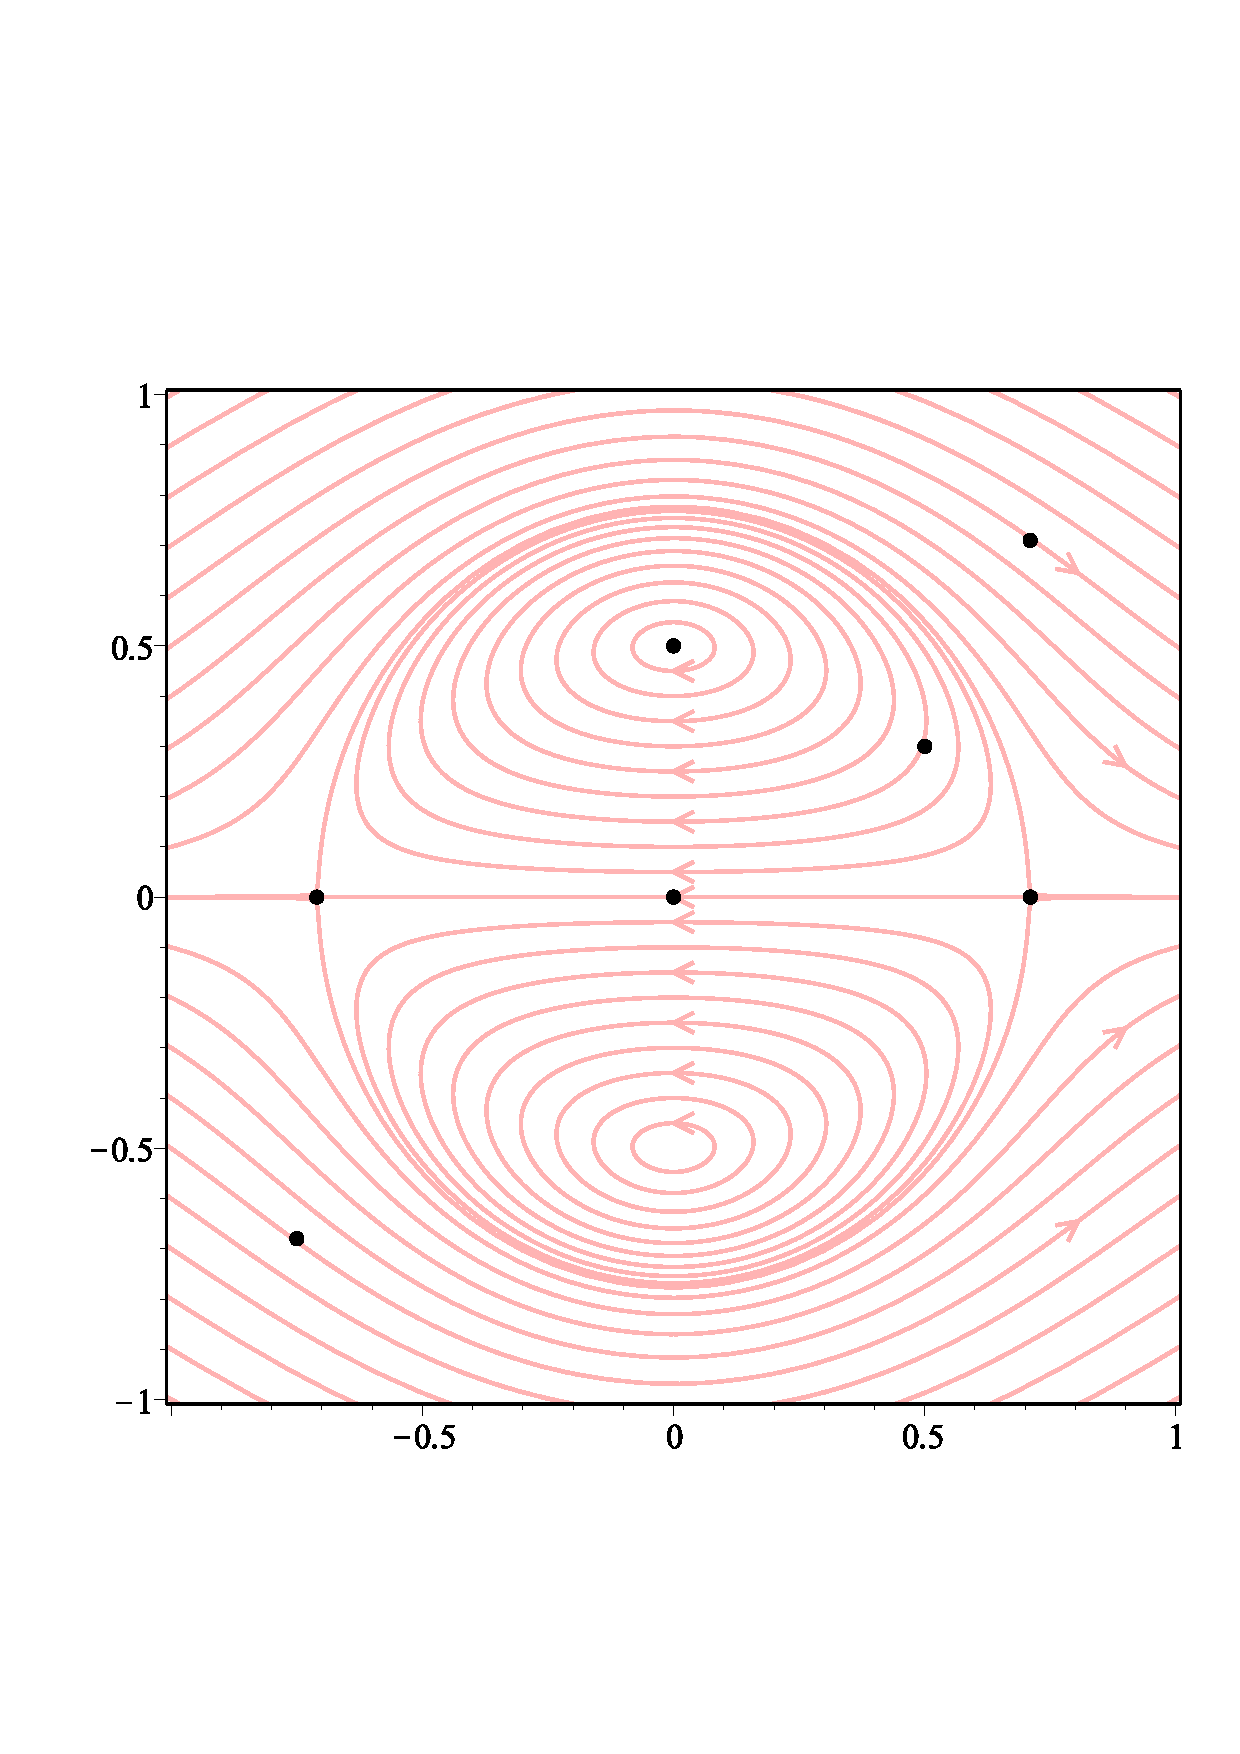
\includegraphics[scale=0.5]{../lectures/images/misc_e_points.pdf}};
   \begin{scope}[xshift=0.40cm,yshift=0.24cm,scale=4.3]
    \draw ( 0.00, 0.00) node[anchor=west]{$A$};
    \draw ( 0.00, 0.50) node[anchor=west]{$B$};
    \draw ( 0.71, 0.00) node[anchor=west]{$C$};
    \draw ( 0.71, 0.71) node[anchor=west]{$D$};
    \draw (-0.71, 0.00) node[anchor=west]{$E$};
    \draw ( 0.50, 0.30) node[anchor=west]{$F$};
    \draw (-0.75,-0.68) node[anchor=west]{$G$};
   \end{scope}
  \end{tikzpicture}
 \end{center}
 Which of the following statements are true?
 \begin{itemize}
  \item[(a)] Point $A$ is an equilibrium point.
  \item[(b)] Point $B$ is a saddle.
  \item[(c)] If a solution has $(x,y)=C$ at $t=0$, then $(x,y)=E$ at
   some time $t>0$.
  \item[(d)] At point $D$ we have $\dot{x}>0$ and $\dot{y}>0$.
  \item[(e)] Point $E$ lies on the $x$-nullcline.
  \item[(f)] If a solution has $(x,y)=F$ at $t=0$, then it also has
   $(x,y)=F$ at some time $t>0$.
  \item[(f)] If a solution has $(x,y)=G$ at $t=0$, then it also has
   $(x,y)=G$ at some time $t>0$.
 \end{itemize}
\end{exercise}
\begin{solution}
 \begin{itemize}
  \item[(a)] This is false.  A solution starting at $A$ will move
   immediately to the left.
  \item[(b)] This is false.  The flow lines near $B$ circulate around
   $B$, so it is a centre, not a saddle.
  \item[(c)] This is false.  Point $C$ is the limit of two different
   flow lines, which means it must be an equilibrium point (and in
   fact a saddle).  This means that a flow line starting at $C$ just
   stays there, it does not move towards $E$.
  \item[(d)] This is false.  The flow line through $D$ points to the
   right (so $\dot{x}>0$) and down (so $\dot{y}<0$).
  \item[(e)] This is true.  In fact $E$ is an equilibrium point (just
   like $C$), so it lies on both the $x$-nullcline and the
   $y$-nullcline.
  \item[(f)] This is true.  The flow line through $F$ is a closed
   curve, so after a finite time the solution starting at $F$ will
   travel all the way around the curve and return to $F$.
  \item[(g)] This is false (assuming that the flow lines behave in the
   obvious way outside the box that we have shown).  The solution
   starting at $G$ will move continually to the right and will never
   return to $G$.
 \end{itemize}
\end{solution}

\begin{exercise}\label{ex-complex-square-a}
 Draw the nullclines and equilibrium points for the following phase
 portrait.
 \[ 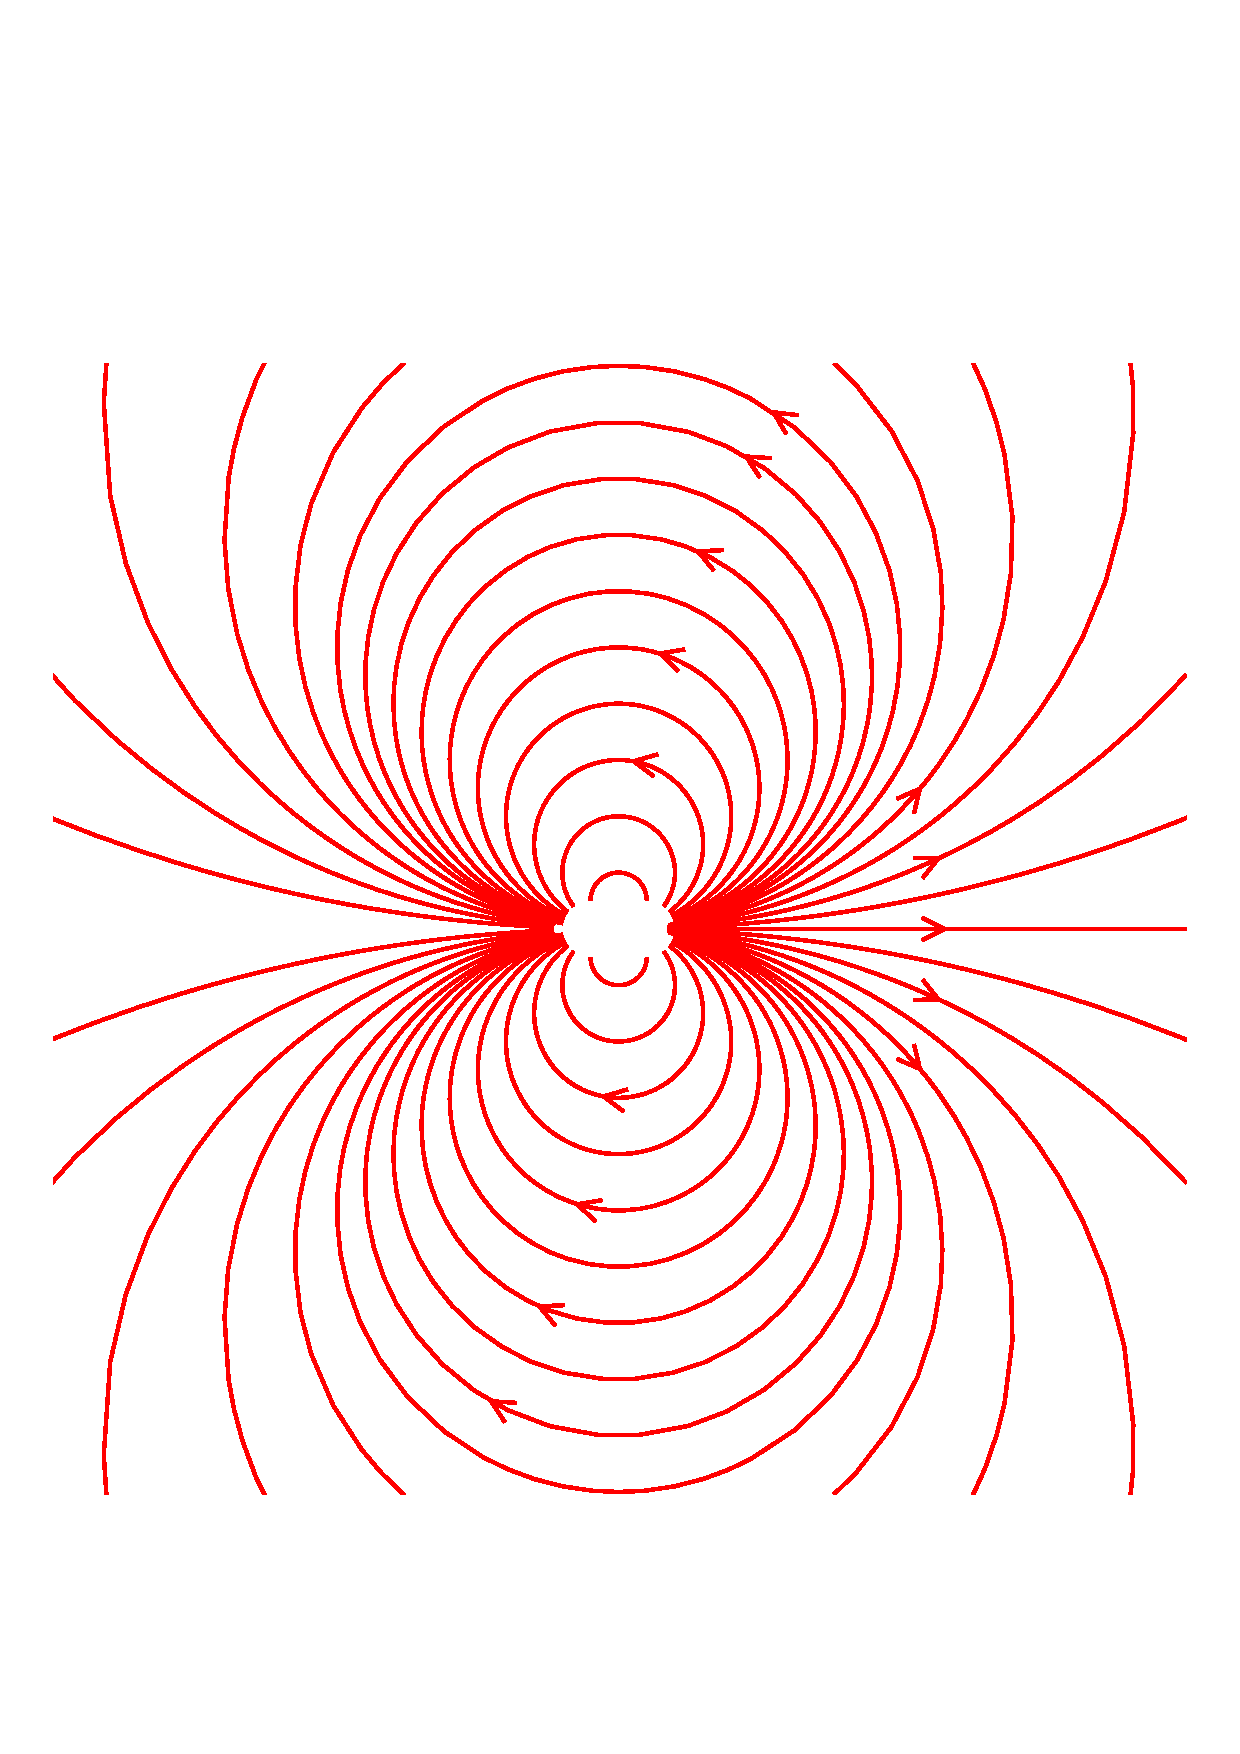
\includegraphics[scale=0.4]{../lectures/images/complex_square_0.pdf} \]
\end{exercise}
\begin{solution}
 Each circular flow line has two points (one on the left and one on
 the right) where the line is vertical and so $\dot{x}=0$.  Joining up
 these points gives the $x$-nullcline, which consists of two diagonal
 lines.  Similarly, at the top and bottom of each circular flow line
 the line is horizontal, so $\dot{y}=0$.  Joining up these points
 gives the $y$-axis, which is part of the $y$-nullcline.  Moreover,
 the whole of the $x$-axis is another flow line which is horizontal
 and so is part of the $y$-nullcline.  Thus, the $y$-nullcline is the
 union of the two axes.
 \[ 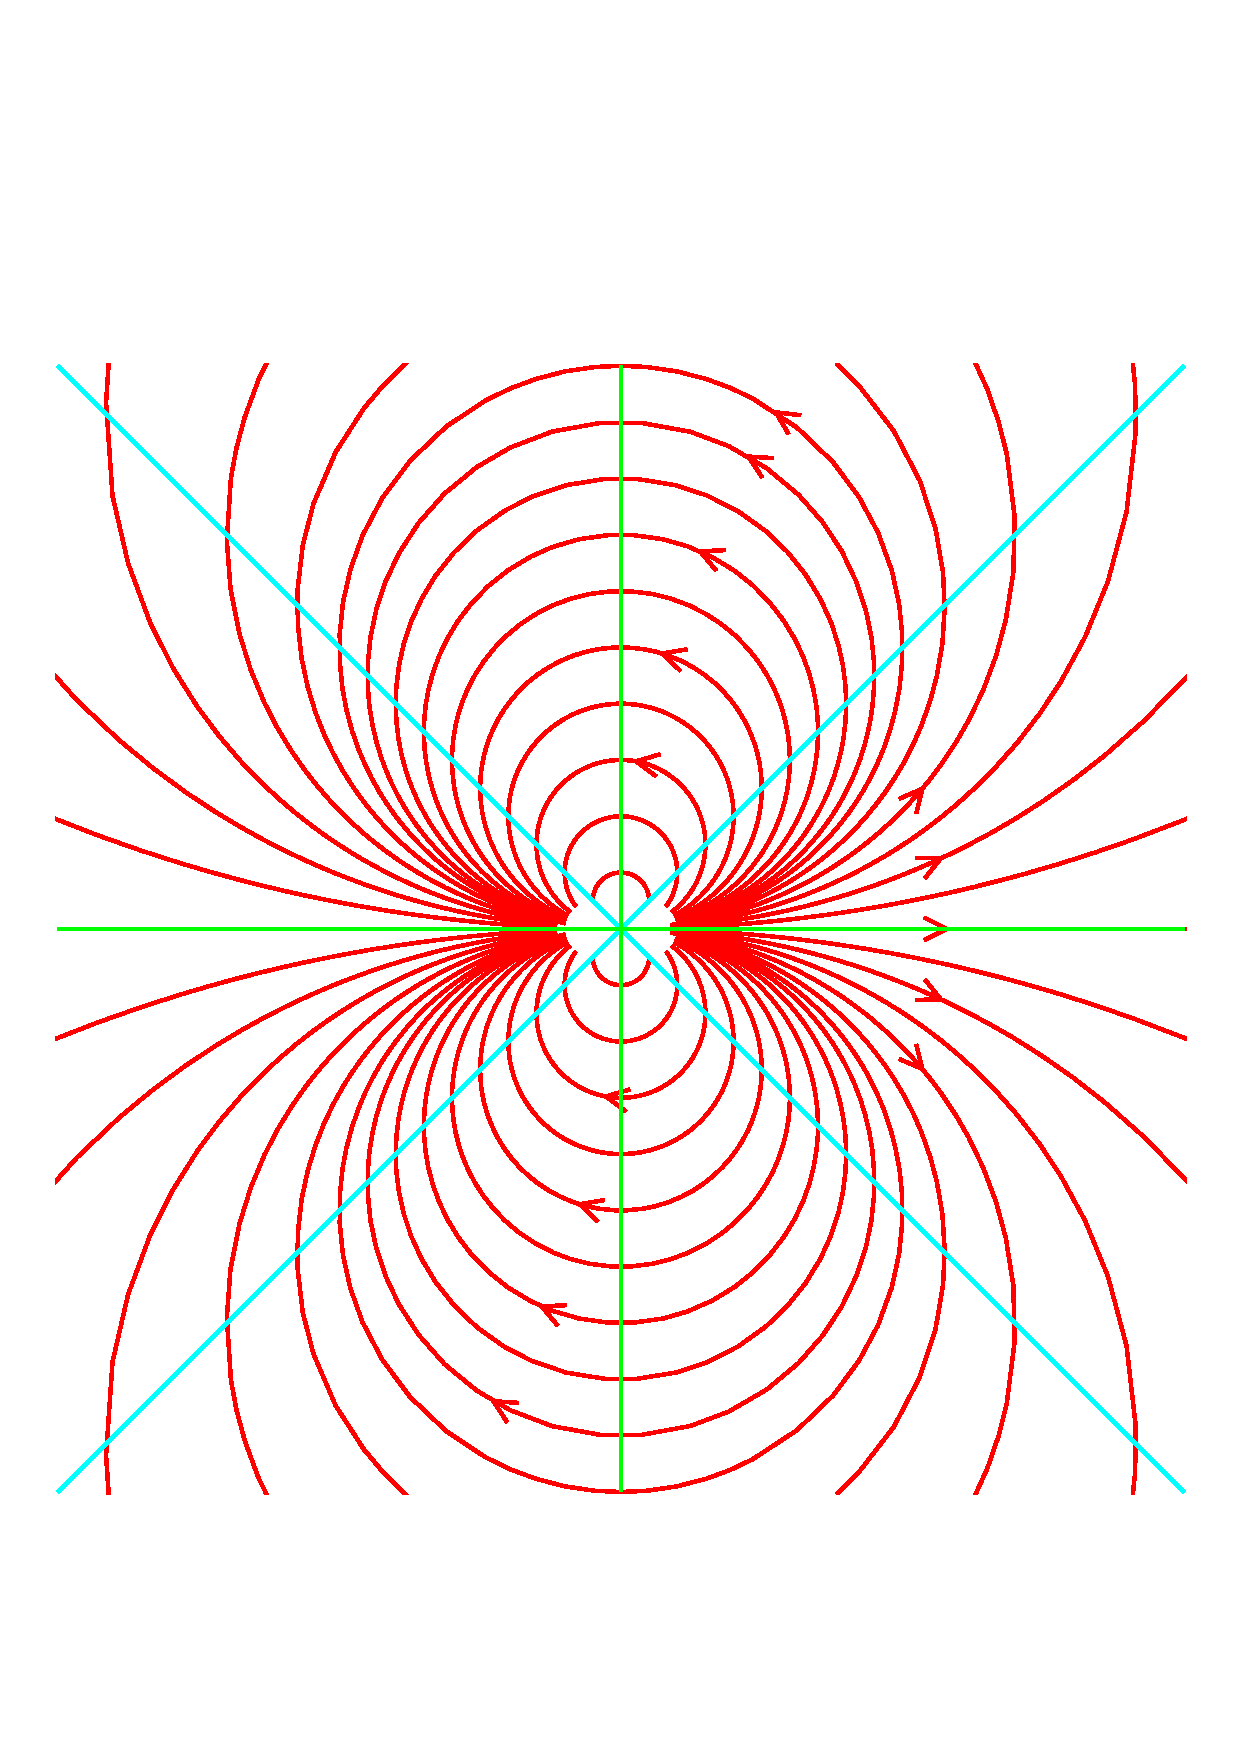
\includegraphics[scale=0.4]{../lectures/images/complex_square.pdf} \]
\end{solution}

\begin{exercise}\label{ex-complex-cube-offset}
 Draw the nullclines and equilibrium points for the following phase
 portrait.
 \[ 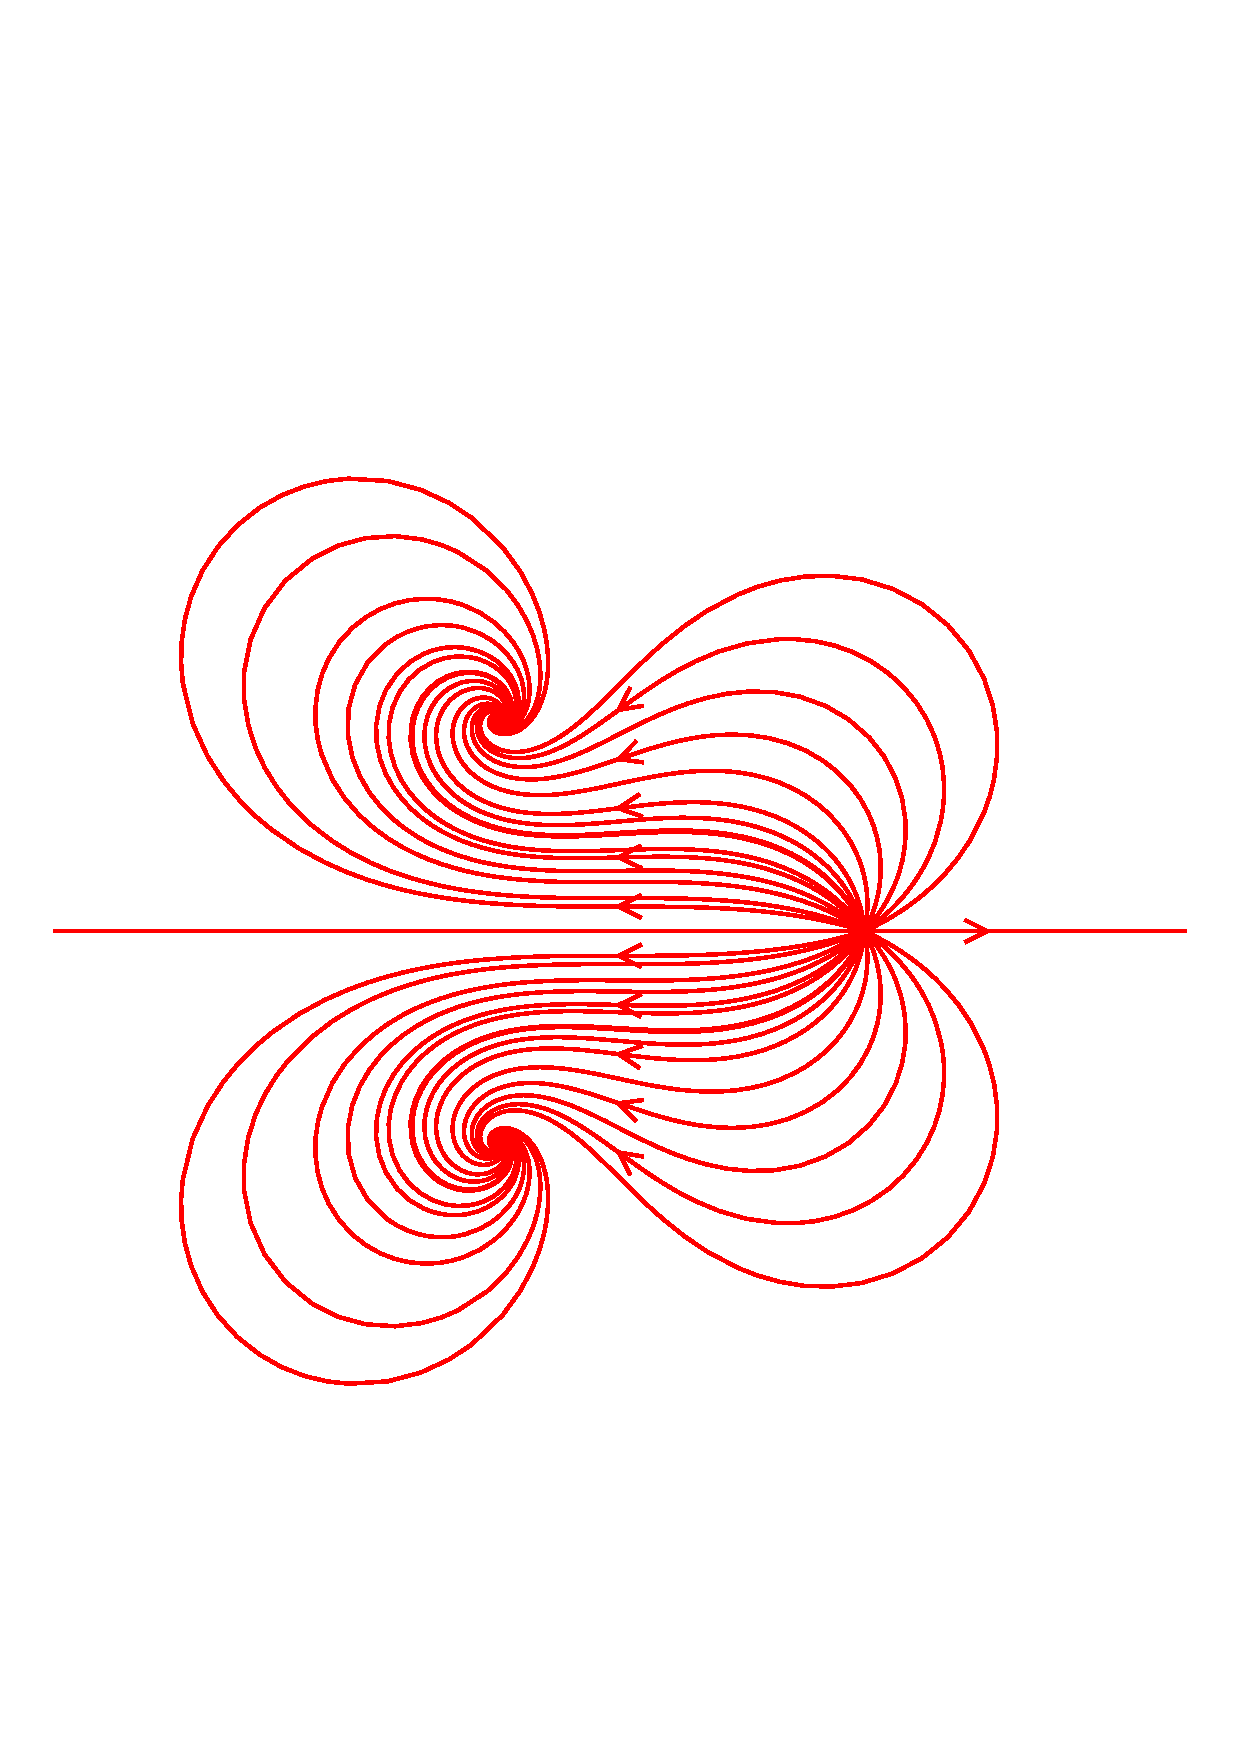
\includegraphics[scale=0.5]{../lectures/images/complex_cube_offset_0.pdf} \]
 Hint: the $y$-nullcline consists of three straight lines, and the
 $x$-nullcline consists of three curves.  The whole picture should be
 very symmetrical.
\end{exercise}
\begin{solution}
 The $x$-axis is a flow line which is horizontal and so is part of the
 $y$-nullcline.  On each of the other flow lines, there is a point
 where the line is horizontal.  These points are easy to find on the
 flow lines that are highly curved, and the hint tells us that we can
 just connect them together with straight lines.  This gives the
 $y$-nullcline.  Similarly, to find the $x$-nullcline, we look for
 points where the flow lines are vertical, and join them together with
 a smooth curve.
 \[ 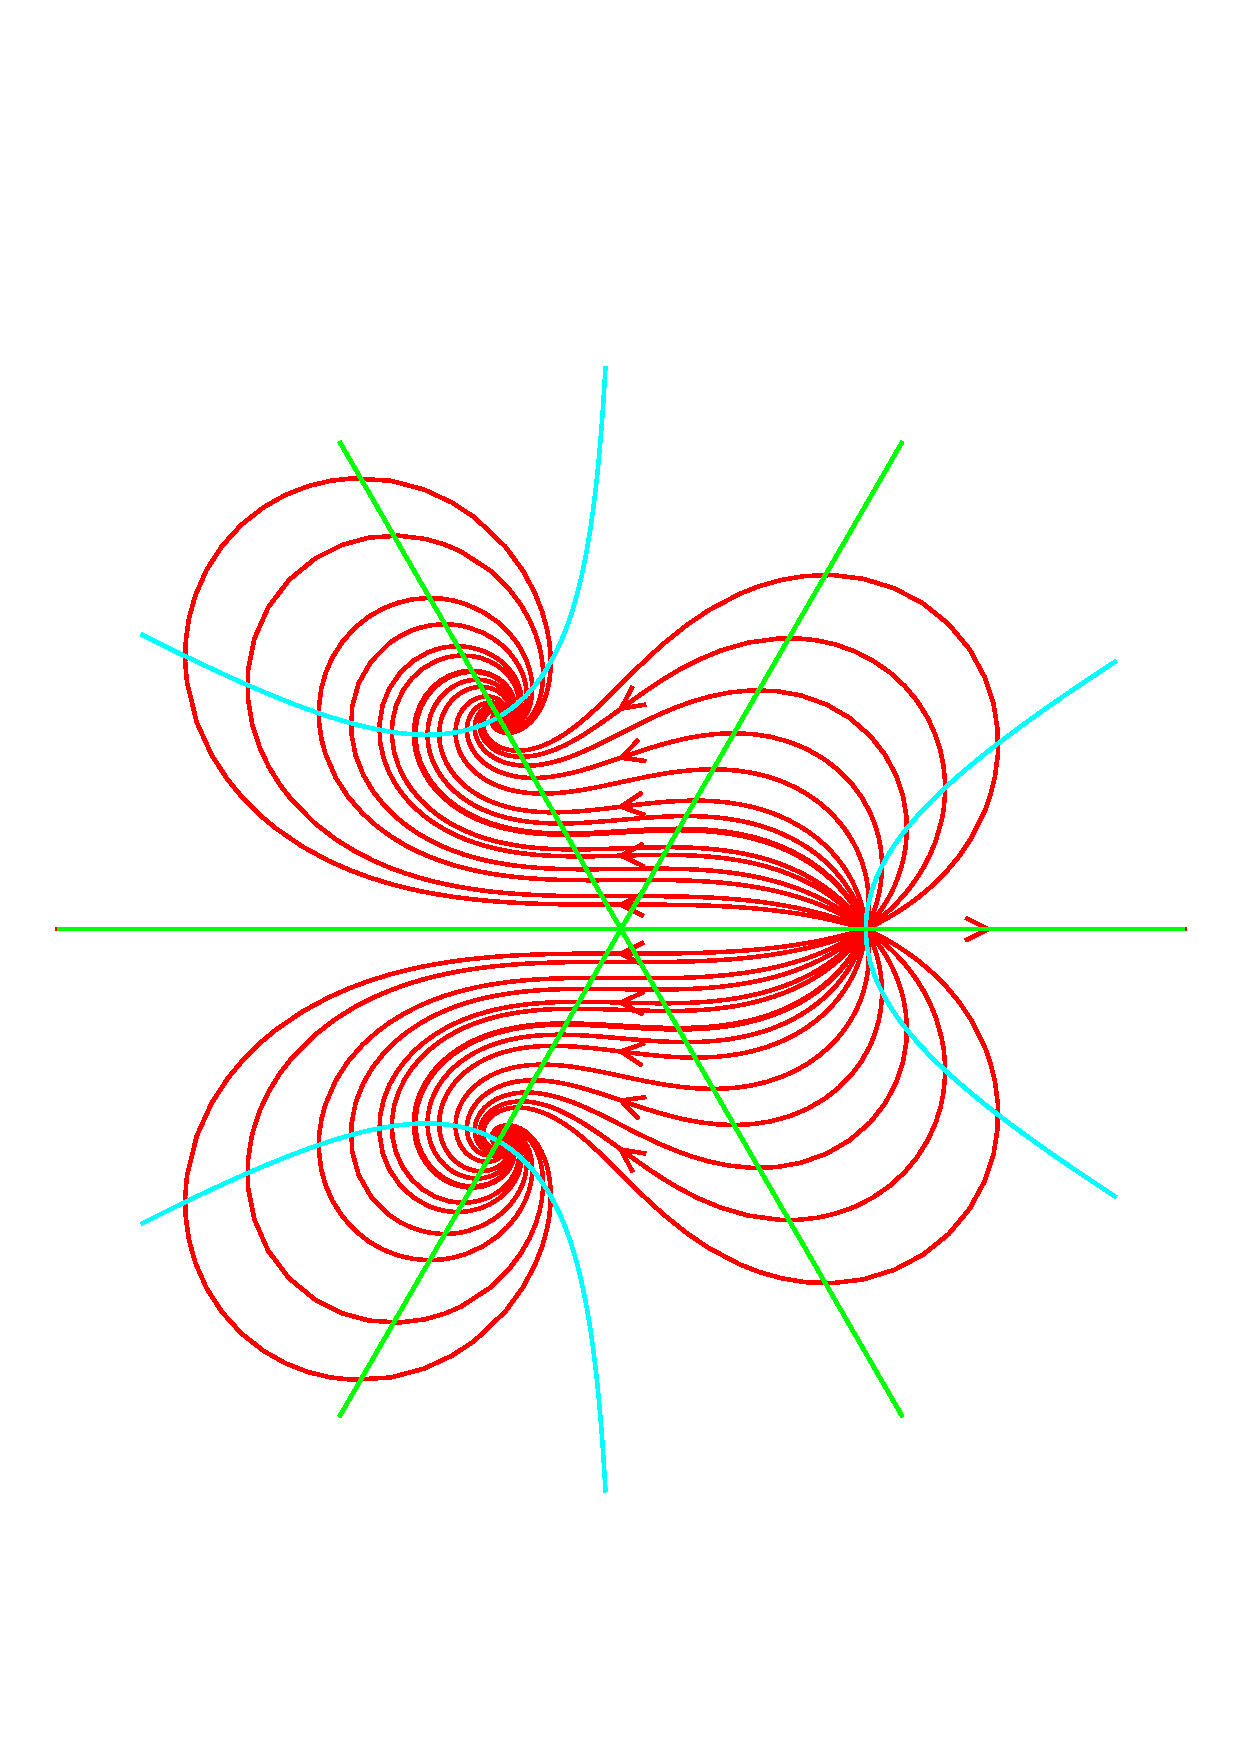
\includegraphics[scale=0.5]{../lectures/images/complex_cube_offset.pdf} \]
\end{solution}

\begin{exercise}\label{ex-which-portrait}
 Consider the following four systems:
 \begin{itemize}
  \item[(a)] $\dot{x}=x^2-y^2$, $\dot{y}=x+1$
  \item[(b)] $\dot{x}=x^2+y^2$, $\dot{y}=x+1$
  \item[(c)] $\dot{x}=x$,\; $\dot{y}=x^2+y^2$
  \item[(d)] $\dot{x}=x^2+2xy-y^2$, $\dot{y}=x^2-2xy-y^2$
 \end{itemize}
 The phase portraits are shown below, in a different order:
 \[ \begin{array}{cccc}
     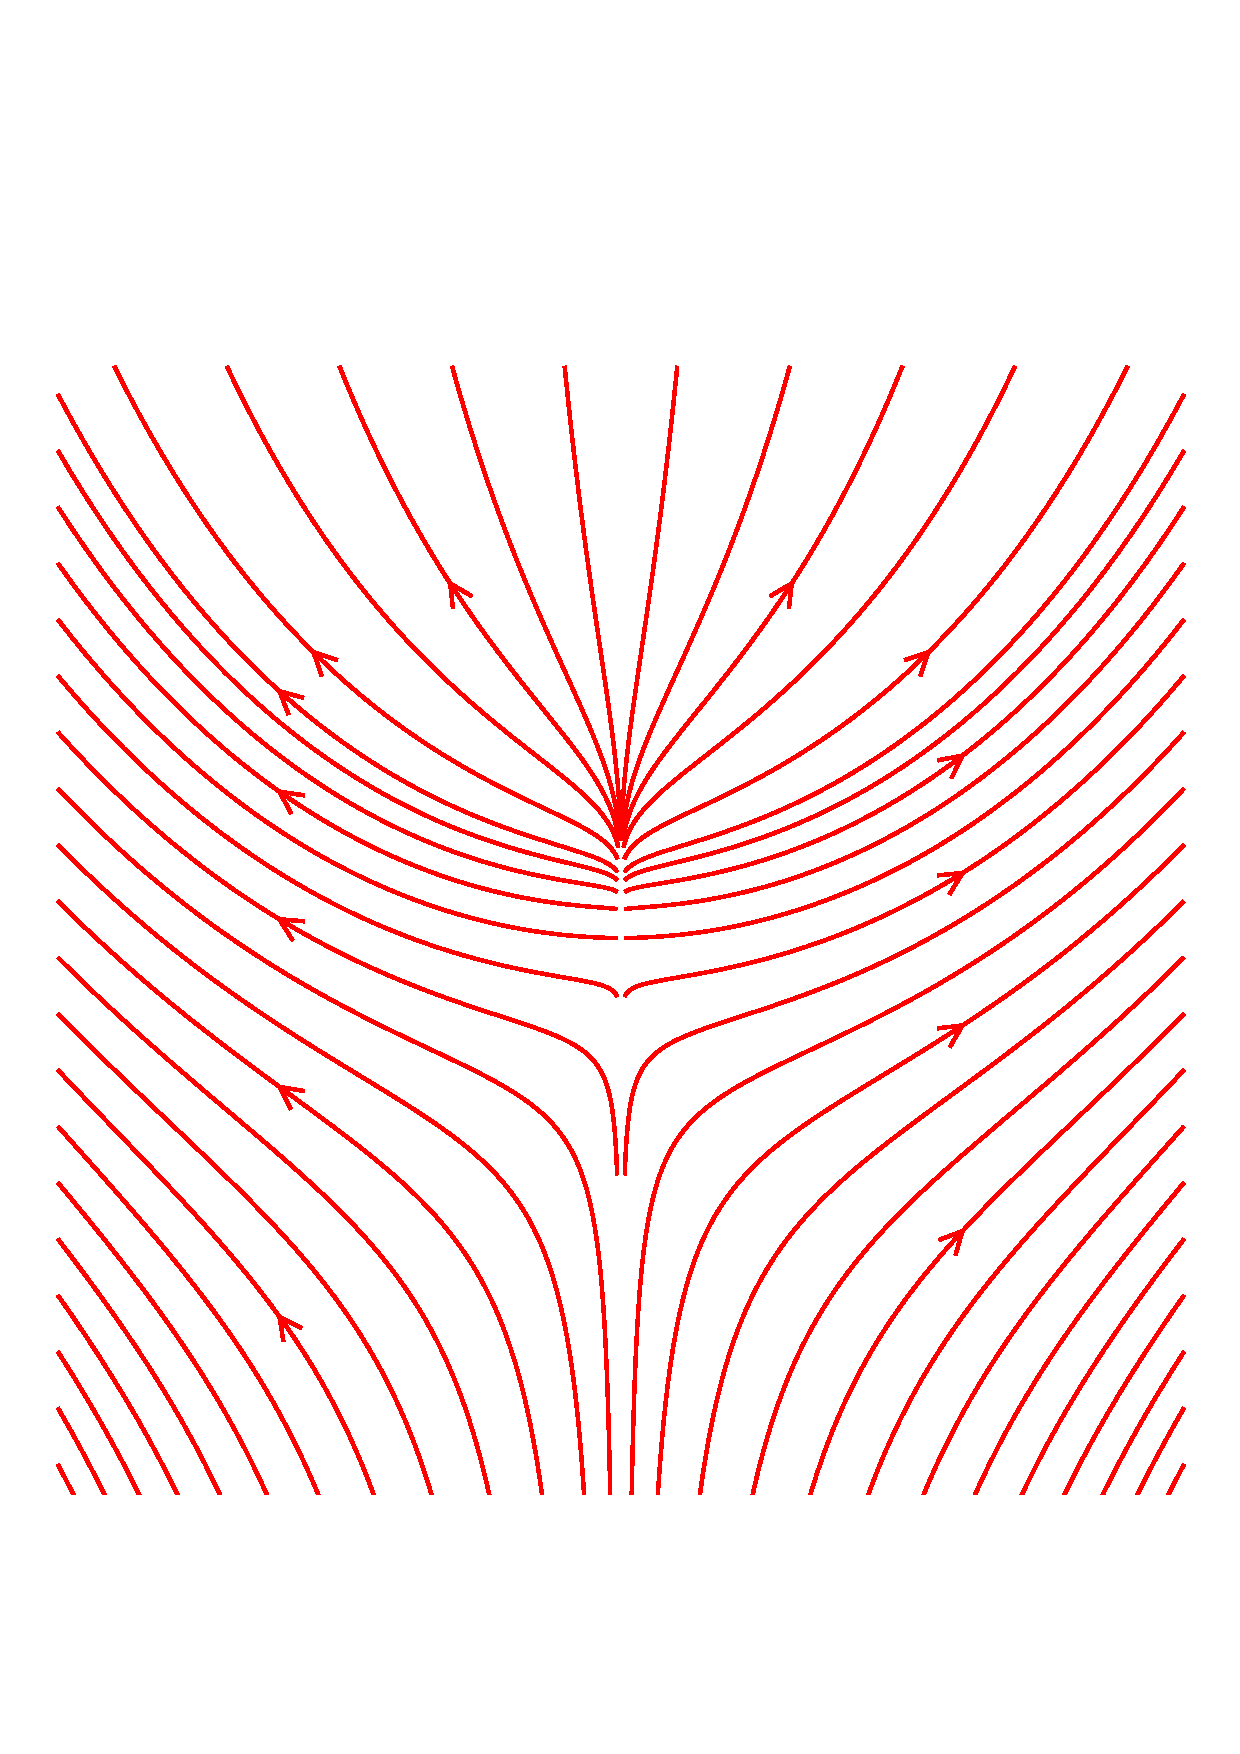
\includegraphics[scale=0.2]{../lectures/images/yggdrasil_0.pdf} &
     \includegraphics[scale=0.2]{../lectures/images/misc_d_0.pdf} &
     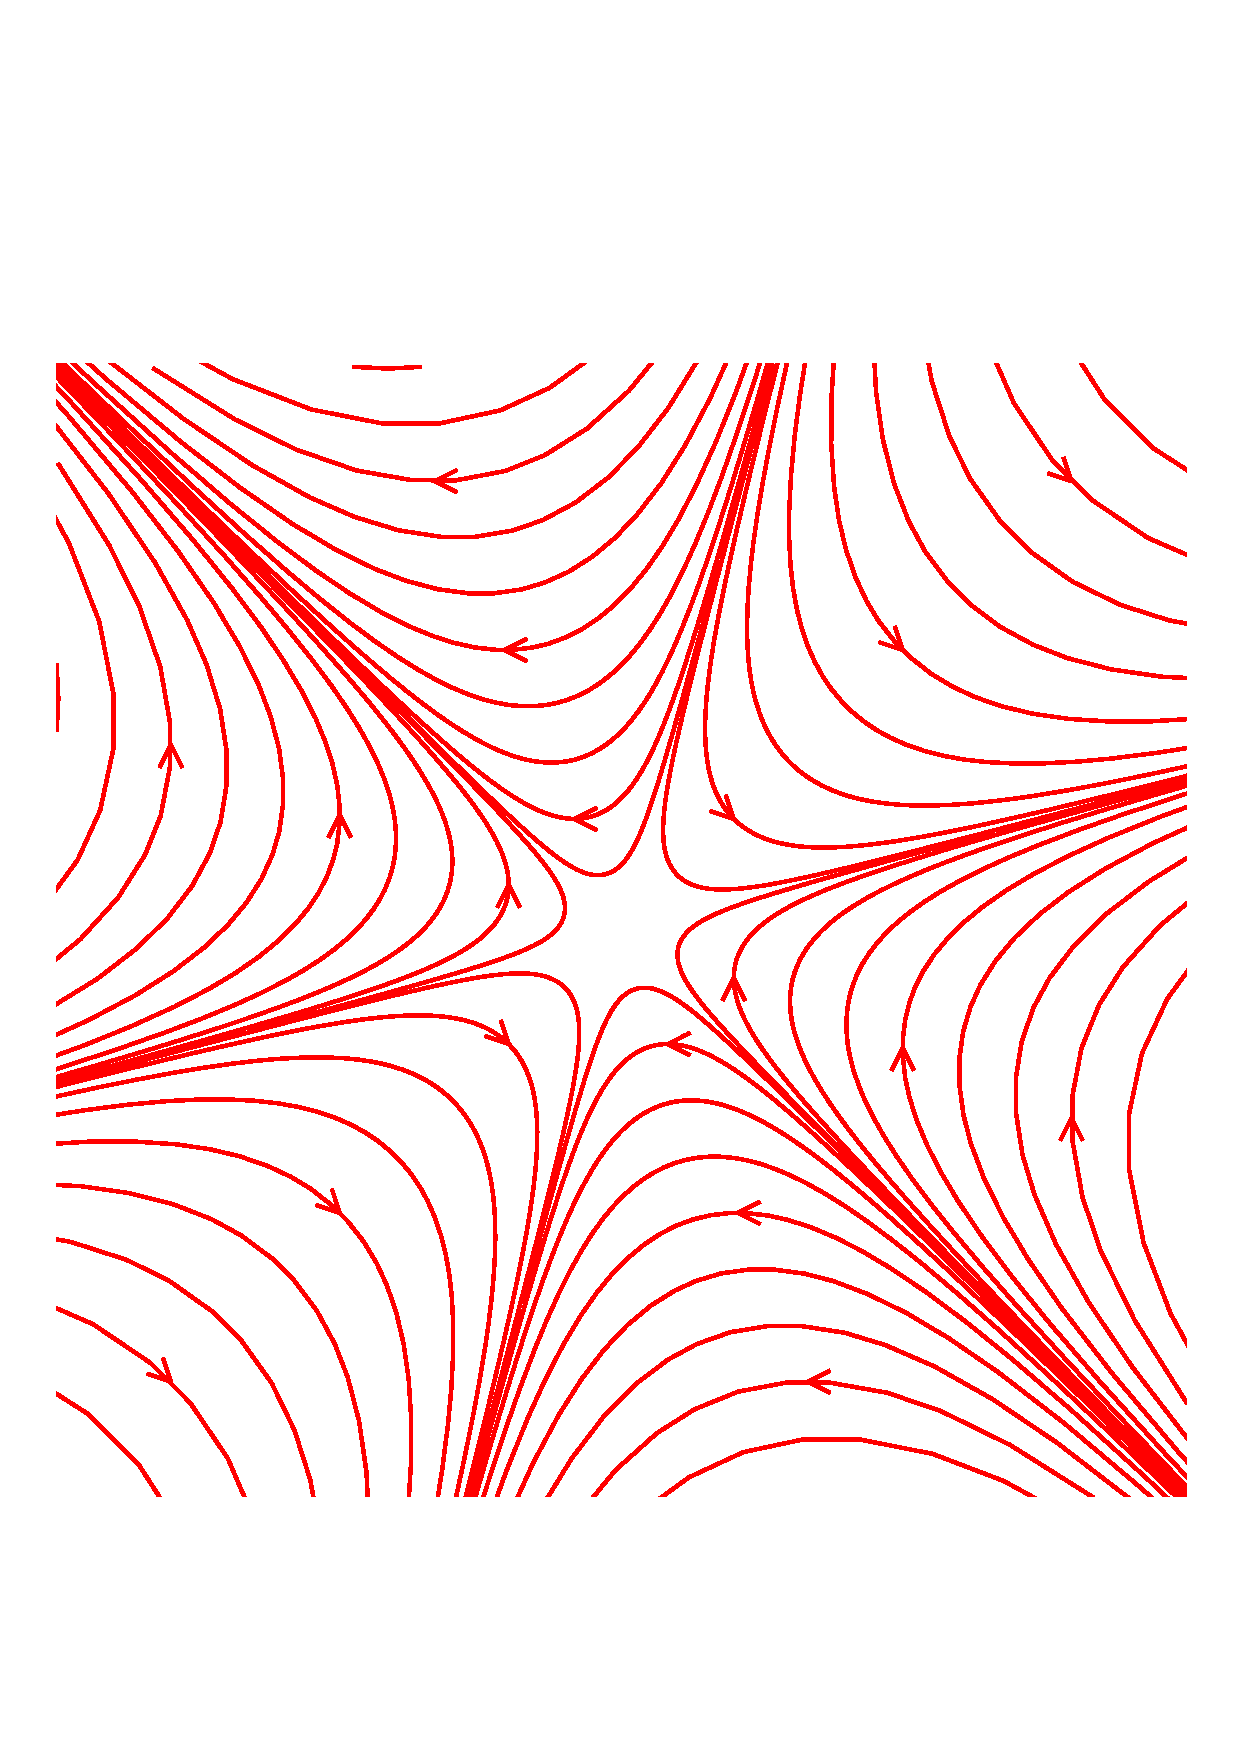
\includegraphics[scale=0.2]{../lectures/images/fluid_0.pdf} &
     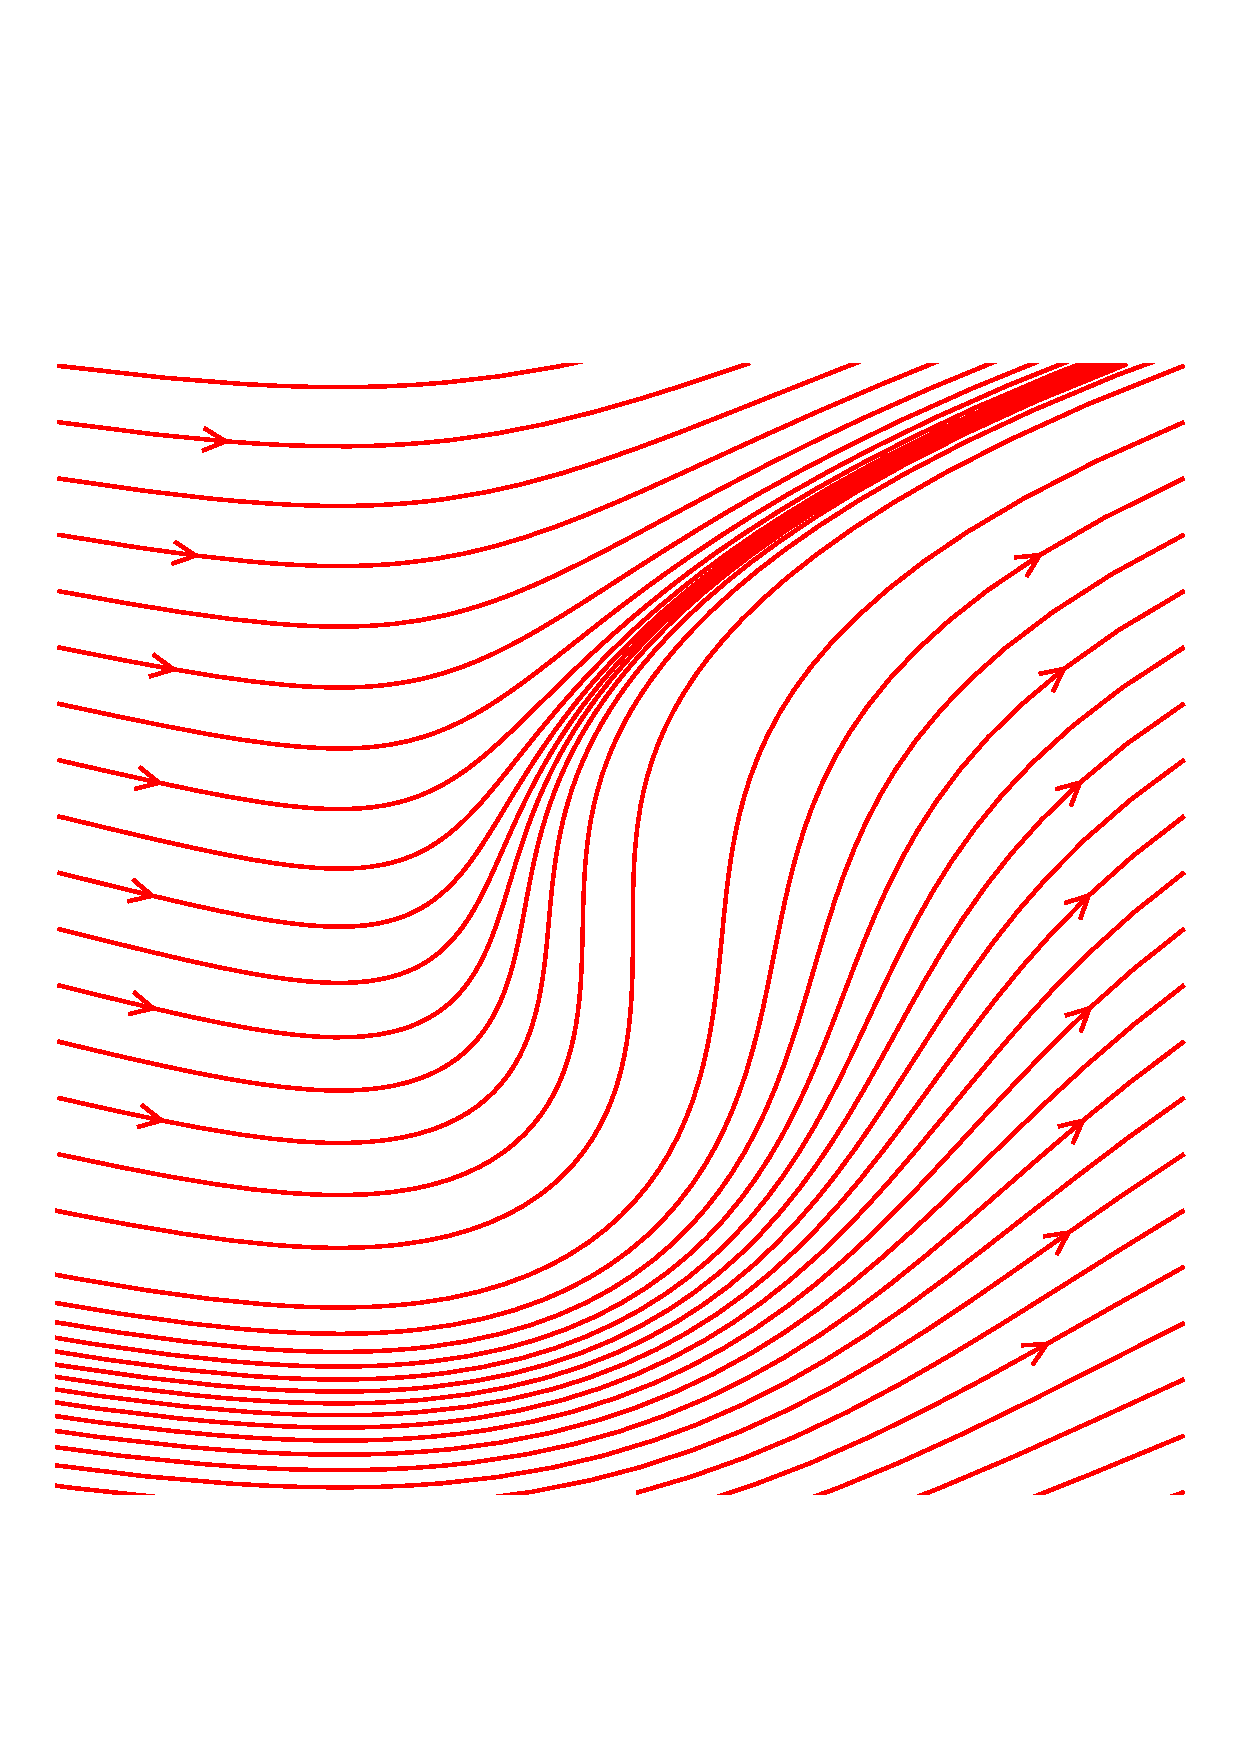
\includegraphics[scale=0.2]{../lectures/images/free_flow_0.pdf} \\
     \text{(p)} & \text{(q)} & \text{(r)} & \text{(s)} 
    \end{array}
 \]
 By considering equilibrium points, nullclines and so on, work out
 which phase portrait belongs to which system.
\end{exercise}
\begin{solution}
 The nullclines and equilibrium points are as follows.
 \begin{itemize}
  \item[(a)] The $x$-nullcline is given by $x^2-y^2=0$, which means
   that $y=\pm x$, so we have two diagonal lines through the origin.
   The $y$-nullcline is given by $x=-1$.  The equilibrium points are
   where $x=-1$ and $y=\pm x$, so they are $(-1,-1)$ and $(-1,1)$.
  \item[(b)] Here the $x$-nullcline is given by $x^2+y^2=0$, which
   is only satisfied when $x=y=0$.  Thus, the $x$-nullcline is a
   single point at the origin.  At all other points we have
   $\dot{x}\geq 0$, so the flow lines move to the right.  The
   $y$-nullcline is a vertical line given by $x=-1$.  The
   $x$-nullcline and the $y$-nullcline do not intersect, so there are
   no equilibrium points. 
  \item[(c)] Here the $y$-nullcline is just a single point at the
   origin, and at all other points the flow lines move upwards.  The
   $x$-nullcline is given by $x=0$.  To the left of this line we have
   $\dot{x}<0$ and so the flow lines move further to the left.
   Similarly, to the right of $x=0$ we have $\dot{x}>0$ and so the
   lines move further to the right.
  \item[(d)] The $x$-nullcline is given by $x^2+2xy-y^2=0$.  This is a
   quadratic equation for $y$, which we can solve to get
   $y=(-2x\pm\sqrt{4x^2+4x^2})/(-2)$, or $y=(1\pm\sqrt{2})x$.  Thus,
   the $x$-nullcline consists of two straight lines through the origin,
   with slopes $1-\sqrt{2}\simeq -0.41$ and
   $1+\sqrt{2}\simeq 2.41$.  Similarly, the $y$-nullcline is given
   by $x^2-2xy-y^2=0$ or $y=(-1\pm\sqrt{2})x$, so it consists of two
   more straight lines through th origin, of slope approximately
   $0.41$ and $-2.41$
 \end{itemize}
 Now consider the pictures.  In picture~(p) the lines all move
 upwards, and they move left when $x<0$ and right when $x>0$; this
 matches with system~(c).  In picture~(q) there are two equilibrium
 points: a saddle near the bottom left, and a focus directly above the
 saddle near the top left.  This matches with the behaviour of
 system~(a).  In picture~(r) we can see that the only equilibrium
 point is at the origin.  We can sketch the $x$-nullcline by looking
 for points where the flow lines are vertical.  We find that these
 points lie on two straight lines through the origin.  Similarly, we
 can sketch that $y$-nullcline by  by looking for points where the
 flow lines are horizontal.  We find that these points again lie on
 two straight lines through the origin.  This matches with
 system~(d).  Finally, picture~(s) shows no equilibrium points at all,
 so this must be system~(b).
\end{solution}

\begin{exercise}\label{ex-spec-a}
 Find the trace, determinant and eigenvalues of the following
 matrices. 
 \[ A = \bbm a & b \\ 0 & c \ebm \hspace{4em}
    B = \bbm \cos(\tht) & -\sin(\tht) \\ \sin(\tht) & \cos(\tht)\ebm \hspace{4em}
    C = \bbm a & b \\ b & a \ebm \hspace{4em}
    D = \bbm 0 & a \\ b & 0 \ebm.
 \]
\end{exercise}
\begin{solution}
 \begin{itemize}
  \item[(a)] Matrix $A$ has trace $\tau=a+c$ and determinant $\dl=ac$,
   so the characteristic polynomial is 
   \[ t^2-\tau t+\dl=t^2-(a+c)t+ac=(t-a)(t-c), \]
   so the eigenvalues are $a$ and $c$.
  \item[(b)] Matrix $B$ has trace
   $\tau=2\cos(\tht)=e^{i\tht}+e^{-i\tht}$ and determinant
   $\dl=\cos(\tht)^2+\sin(\tht)^2=1$.  It follows that the
   characteristic polynomial is 
   \[ t^2-\tau t+\dl= t^2 - (e^{i\tht}+e^{-i\tht})t+1 = 
       (t-e^{i\tht})(t-e^{-i\tht}),
   \]
   and the eigenvalues are $e^{i\tht}$ and $e^{-i\tht}$.
  \item[(c)] Matrix $C$ has trace $\tau=2a$ and determinant
   $\dl=a^2-b^2$.  It follows that $\tau^2-4\dl=4a^2-4a^2+4b^2=4b^2$,
   so the eigenvalues are 
   \[ \half(\tau\pm\sqrt{\tau^2-4\dl}) = \half(2a\pm 2b) = a+b,\;a-b. \]
  \item[(d)] Matrix $D$ has trace $\tau=0$ and determinant $\dl=-ab$,
   so the characteristic polynomial is $t^2-ab$, and the eigenvalues
   are $\pm\sqrt{ab}$.
 \end{itemize}
\end{solution}

\begin{exercise}\label{ex-linear-a}
 Solve the system $\dot{u}=13v$, $\dot{v}=-13u-10v$ with
 $u=a$ and $v=b$ at $t=0$.
\end{exercise}
\begin{solution}
 The problem can be written as
 $\bbm\dot{u}\\ \dot{v}\ebm=A\bbm u\\ v\ebm$, where 
 $A=\bbm 0 & 13 \\ -13 & -10\ebm$.  The trace is $\tau=-10$ and the
 determinant is $\dl=13^2=169$, so $\tau^2-4\dl=-576<0$.  Thus, the
 eigenvalues are $(-10\pm\sqrt{576}i)/2=-5\pm 12i$.  We therefore have
 a stable focus with $\lm=-5$ and $\om=12$.  The corresponding matrix
 $P$ is
 \[ P = e^{\lm t}(\cos(\om t)I+\om^{-1}\sin(\om t)(A-\lm I))
      = e^{-5t}(\cos(12t)I+\frac{1}{12}\sin(12t)(A+5I)).
 \]
 Here 
 \[ \frac{A+5I}{12} = 
     \frac{1}{12}\bbm 5 & 13 \\ -13 & -5 \ebm = 
      \bbm 5/12 & 13/12 \\ -13/12 & -5/12 \ebm, 
 \]
 so 
 \[ P = e^{-5t}\bbm \cos(12t)+\frac{5}{12}\sin(12t) & 
                    \frac{13}{12}\sin(12t) \\
                    -\frac{13}{12}\sin(12t) &
                    \cos(12t)-\frac{5}{12}\sin(12t) \ebm.
 \]
 Thus, the solution starting at $\bbm a\\ b\ebm$ is
 \[ \bbm u\\ v \ebm = P\bbm a\\ b\ebm =
      e^{-5t} \bbm a\cos(12t) + \frac{5a+13b}{12}\sin(12t) \\
                   b\cos(12t) - \frac{13a+5b}{12}\sin(12t) \ebm.
 \]
\end{solution}

\begin{exercise}\label{ex-linear-equilibria}
 For each of the following linear systems, classify the equilibrium
 point at the origin.
 \begin{itemize}
  \item[(a)] $\dot{x}=2x+y$, $\dot{y}=x+2y$
  \item[(b)] $\dot{x}=2x+y$, $\dot{y}=x-3y$
  \item[(c)] $\dot{x}=x-4y$, $\dot{y}=2x-y$
  \item[(d)] $\dot{x}=2y$,   $\dot{y}=-3x-y$
  \item[(e)] $\dot{x}=8y-x$, $\dot{y}=7y-2x$
  \item[(f)] $\dot{x}=3y-7x$, $\dot{y}=3y-8x$.
 \end{itemize}
\end{exercise}
\begin{solution}
 \[ \renewcommand{\arraystretch}{1.5}
    \begin{array}{|c|c|c|c|c|c|c|} \hline
     \text{ system } & A & \tau & \dl & \tau^2-4\dl & \lm_1,\lm_2 & \text{ type } \\ \hline
     \text{(a)} & \bbm  2& 1\\ 1& 2\ebm &  4 &  3 &   4 & 1,3 & \text{ unstable node } \\ \hline
     \text{(b)} & \bbm  2& 1\\ 1&-3\ebm & -1 & -7 &  29 & \frac{-1\pm\sqrt{29}}{2} & \text{ saddle } \\ \hline
     \text{(c)} & \bbm  1&-4\\ 2&-1\ebm &  0 &  7 & -28 & \pm\sqrt{7}i & \text{ centre } \\ \hline
     \text{(d)} & \bbm  0& 2\\-3&-1\ebm & -1 &  6 & -23 & \frac{-1\pm\sqrt{23}i}{2} & \text{ stable focus } \\ \hline
     \text{(e)} & \bbm -1& 8\\-2& 7\ebm &  6 &  9 &   0 & 3,3 & \text{ unstable node } \\ \hline
     \text{(f)} & \bbm -7& 3\\-8& 3\ebm & -4 &  3 &   4 & -3,-1 & \text{ stable node } \\ \hline
    \end{array}
 \]
\end{solution}

\begin{exercise}\label{ex-classify-omni}
 Suppose we have five different linear differential equations with
 properties described below.  In each case, find the type of
 equilibrium point at the origin.
 \begin{itemize}
  \item The matrix for system A has eigenvalues $-2$ and $3$.
  \item The matrix for system B has $\tau=0$ and $\dl=16$.
  \item One of the solutions for system C is
   $\bbm x\\ y\ebm = \bbm 3e^{-2t}+2e^{-3t} \\ 3e^{-3t}+2e^{-2t}\ebm$.
  \item System D has the following phase portrait:
   \[ 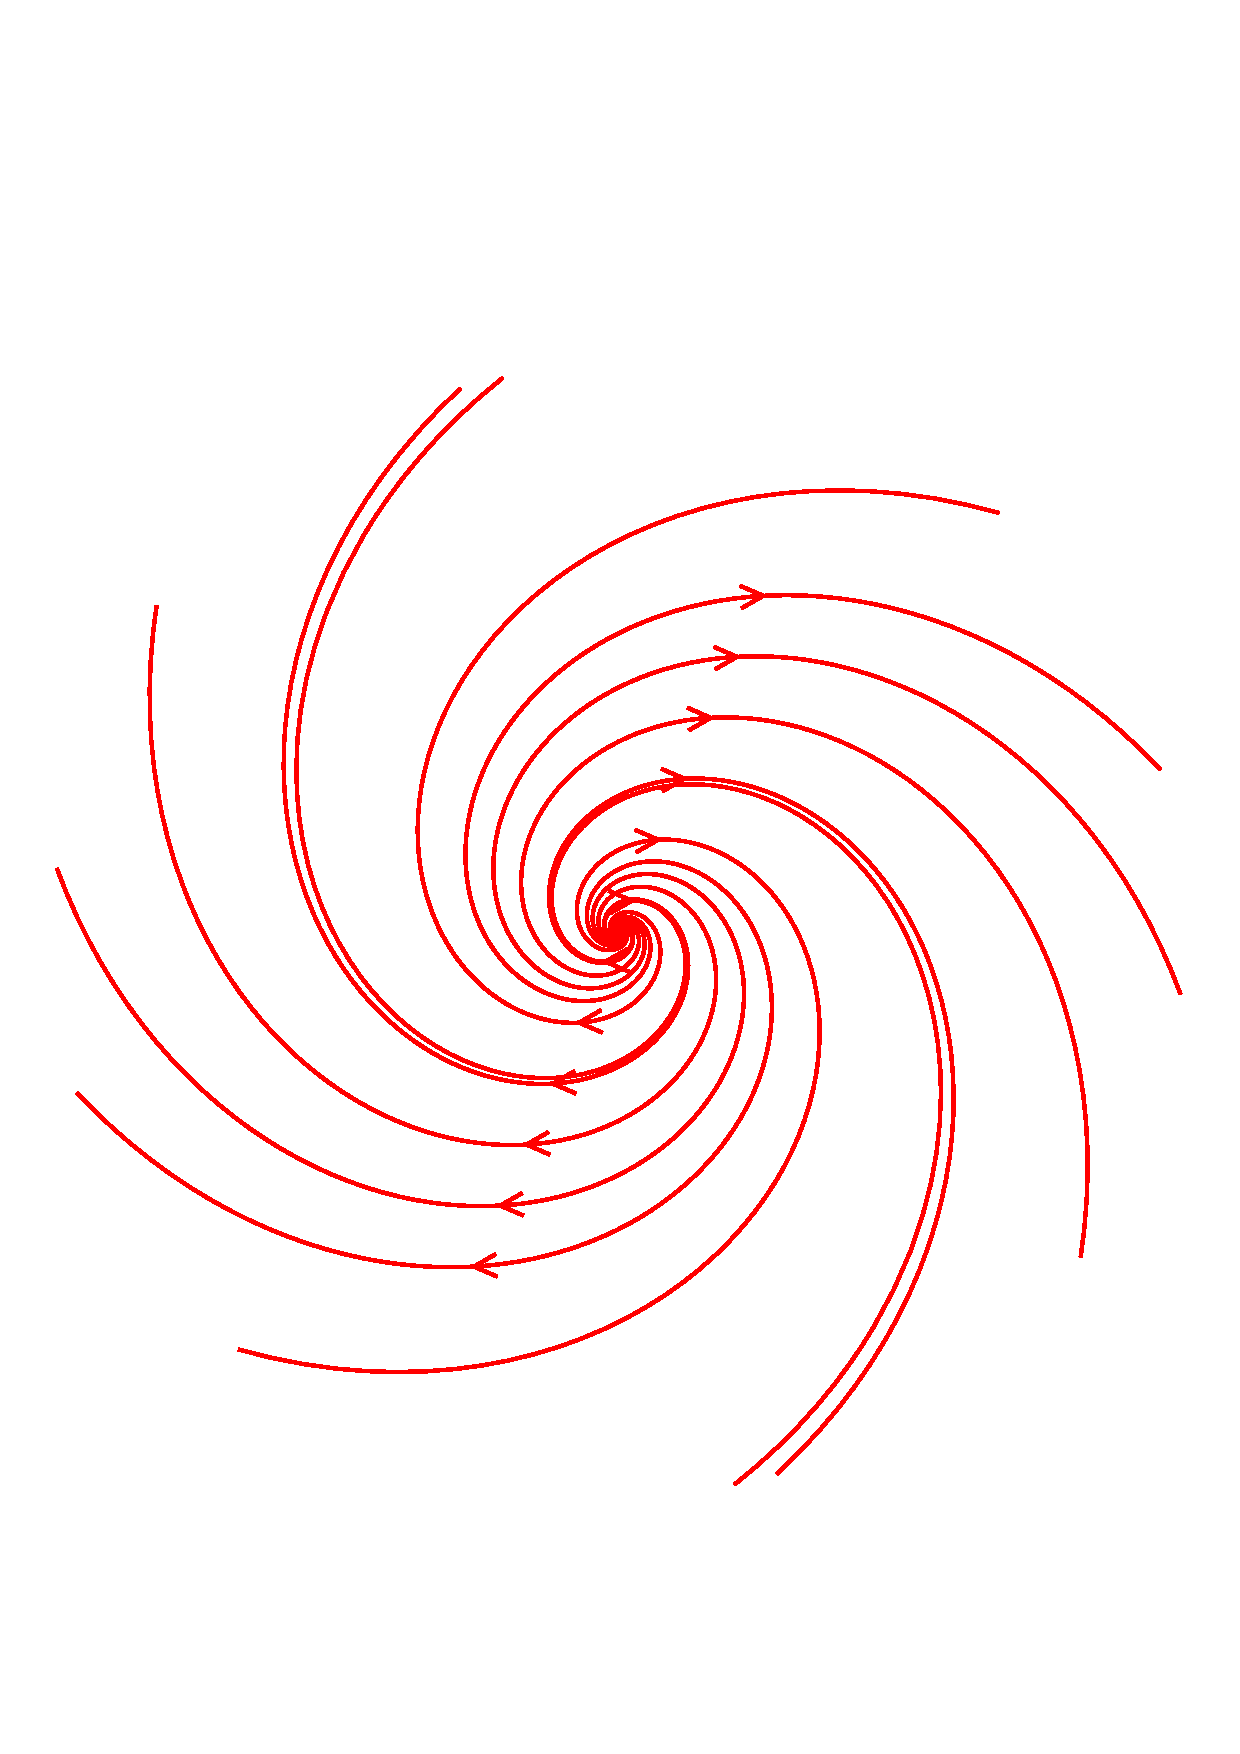
\includegraphics[scale=0.2]{../lectures/images/simple_clockwise_unstable_focus.pdf} \]
  \item System E corresponds to the following point in the
   $(\tau,\dl)$ plane:
   \begin{center}
    \begin{tikzpicture}[scale=2.5]
     \draw[thick,cyan] (-1,0) -- (0,0);
     \draw[thick,orange,->] (0,0) -- (1,0);
     \draw[thick,olivegreen,->] (0,0) -- (0,1);
     \draw[thick,blue,smooth] (-1,1) -- (-0.9,0.81) -- (-0.8,0.64) --
       (-0.7,0.49) -- (-0.6,0.36) -- (-0.5,0.25) -- (-0.4,0.16) --
       (-0.3,0.09) -- (-0.2,0.04) -- (-0.1,0.01) -- (0,0);
     \draw[thick,red,smooth] (1,1) -- (0.9,0.81) -- (0.8,0.64) --
       (0.7,0.49) -- (0.6,0.36) -- (0.5,0.25) -- (0.4,0.16) --
       (0.3,0.09) -- (0.2,0.04) -- (0.1,0.01) -- (0,0);
     \draw(0,1) node[anchor=south]{$\ss\dl$};
     \draw(1,0) node[anchor=west]{$\ss\tau$};
     \fill[black] (0.8,0.2) circle(0.02);
    \end{tikzpicture}
   \end{center}
 \end{itemize}
\end{exercise}
\begin{solution}\leavevmode
 \begin{itemize}
  \item[A] This system has one negative eigenvalue and one positive
   eigenvalue, so it must be a saddle.
  \item[B] This system has $\tau=0$ and $\dl>0$ so it is a centre.
   The eigenvalues are $\pm\sqrt{-4\tm 16}=\pm 8i$, so the angular
   frequency is $\om=8$.  We do not have enough information to decide
   whether the rotation is clockwise or anticlockwise.
  \item[C] As $e^{-2t}$ and $e^{-3t}$ appear in the solution, the
   eigenvalues must be $-2$ and $-3$.  As these are both negative real
   numbers, we have a stable node.
  \item[D] As the flow lines spiral outwards, this is an unstable
   focus.
  \item[E] The given point is in the top right quadrant where $\tau>0$
   and $\dl>0$.  It lies below the parabola with equation
   $\dl=\tau^2/4$, so $\dl<\tau^2/4$, so $\tau^2-4\dl>0$.  This means
   that the eigenvalues $(\tau\pm\sqrt{\tau^2-4\dl})/2$ are both
   positive, so we have an unstable node.
 \end{itemize}
\end{solution}

\begin{exercise}\label{ex-linear-find-eg-a}
 Give examples of linear differential equations of the following
 types.  Try to make your examples as simple as possible.
 \begin{itemize}
  \item[(a)] A stable node.
  \item[(b)] A saddle.
  \item[(c)] A clockwise centre.
  \item[(d)] An anticlockwise unstable focus.
 \end{itemize}
\end{exercise}
\begin{solution}\leavevmode
 \begin{itemize}
  \item[(a)] We need a system with two distinct, negative
   eigenvalues.  The simplest example is the matrix
   $\bbm -1&0\\0&-2\ebm$, or the corresponding system $\dot{x}=-x$, 
   $\dot{y}=-2y$. 
  \item[(b)] We need a system with one positive eigenvalue and one
   negative eigenvalue.  The simplest example is the matrix
   $\bbm 1&0\\0&-1\ebm$, or the corresponding system $\dot{x}=x$,
   $\dot{y}=-y$.
  \item[(c)] We need a system with $\tau=0$ and $\dl>0$.  The two
   simplest examples are $\bbm 0&-1\\ 1&0\ebm$ and 
   $\bbm 0&1\\-1&0\ebm$.  The first of these gives an anticlockwise
   rotation, so we use the second one.  The corresponding equations
   are $\dot{x}=y$ and $\dot{y}=-x$.
  \item[(d)] We need a system with $\tau^2-4\dl<0$ (for a focus) and
   $\tau>0$ (to make it unstable).  The bottom left entry in the
   matrix should also be positive, to ensure that the rotation is
   anticlockwise.  A simple example is $\bbm 0&-1\\1&1\ebm$, which has
   $\tau=\dl=1$.  The corresponding equations are $\dot{x}=-y$ and
   $\dot{y}=x+y$.  
 \end{itemize}
\end{solution}

\begin{exercise}\label{ex-diagonalise}
 Consider the matrix $A=\bbm -4 & 3 \\ -10 & 7 \ebm$.
 \begin{itemize}
  \item[(a)] Find the trace, determinant, eigenvalues and eigenvectors
   of $A$.
  \item[(b)] Hence find a diagonal matrix $D$ and an invertible matrix
   $V$ such that $A=VDV^{-1}$.
  \item[(c)] Find a matrix $P$ depending on $t$ such that $P=I$ when
   $t=0$, and $\dot{P}=AP$.
  \item[(d)] Find a vector $u$ depending on $t$ such that
   $u=\bbm 1\\ 1\ebm$ at $t=0$, and $\dot{u}=Au$.
 \end{itemize}
\end{exercise}
\begin{solution}\leavevmode
 \begin{itemize}
  \item[(a)] The trace is $\tau=-4+7=3$, and the determinant is
   $\dl=(-4)\tm 7-3\tm(-10)=2$.  This means that $\tau^2-4\dl=9-8=1$.
   The eigenvalues are $(\tau\pm\sqrt{\tau^2-4\dl})/2$, which gives
   $\lm_1=1$ and $\lm_2=2$.  An eigenvector $v_1$ of eigenvalue $1$
   must satisfy $(A-I)v_1=0$, but $A-I=\bbm -5&3 \\ -10&6\ebm$, so we
   can take $v_1=\bbm 3\\ 5\ebm$.  Similarly, an eigenvector $v_2$ of
   eigenvalue $2$ must satisfy $(A-2I)v_2=0$, but
   $A-2I=\bbm -6&3 \\ -10&5\ebm$, so we can take $v_2=\bbm 1\\ 2\ebm$.
  \item[(b)] The general method here is to take 
   \begin{align*}
    V &= \barmat{v_1}{v_2} = \bbm 3 & 1 \\ 5 & 2 \ebm \\
    D &= \bbm \lm_1 & 0 \\ 0 & \lm_2 \ebm = \bbm 1&0 \\ 0&2 \ebm.
   \end{align*}
   Note here that $\det(V)=3\tm 2 - 1\tm 5=1$ and so 
   \[ V^{-1} = \bbm 2 & -1 \\ -5 & 3 \ebm. \]
  \item[(c)] In the lectures we gave two different methods for this.
   The first method says that $P=VEV^{-1}$, where 
   \[ E=\bbm e^{\lm_1t} & 0 \\ 0 & e^{\lm_2t} \ebm =
        \bbm e^t & 0 \\ 0 & e^{2t} \ebm.
   \]
   This works out as 
   \[ P = \bbm 3 & 1 \\ 5 & 2 \ebm
          \bbm e^t & 0 \\ 0 & e^{2t} \ebm
          \bbm 2 & -1 \\ -5 & 3 \ebm 
        = \bbm 3 & 1 \\ 5 & 2 \ebm
          \bbm 2e^t & -e^t \\ -5e^{2t} & 3e^{2t} \ebm 
        = \bbm 6e^t-5e^{2t} & -3e^t+3e^{2t} \\
               10e^t - 10e^{2t} & -5e^t + 6e^{2t} \ebm.
   \]
   The second approach uses the formula
   \[ P=(\lm_2-\lm_1)^{-1}((\lm_2e^{\lm_1t}-\lm_1e^{\lm_2t})I +
                        (e^{\lm_2t}-e^{\lm_1t})A).
   \]
   In our case this becomes
   \begin{align*}
    P &= (2e^t-e^{2t})I + (e^{2t}-e^t)A \\
      &= \bbm 2e^t-e^{2t} & 0 \\ 0 & 2e^t-e^{2t} \ebm +
         (e^{2t}-e^t)\bbm -4 & 3 \\ -10 & 7 \ebm 
       = \bbm 6e^t - 5e^{2t} & -3e^t + 3e^{2t} \\
              10e^t - 10e^{2t} & -5 e^t + 6 e^{2t} \ebm.
   \end{align*}
  \item[(d)] The relevant vector is 
   $u=P\bbm 1\\ 1\ebm = \bbm 3e^t - 2e^{2t}\\ 5e^t - 4e^{2t}\ebm$
 \end{itemize}
\end{solution}

\begin{exercise}\label{ex-fundamental-a}
 For each of the following matrices $A_k$, find a matrix
 $P_k$ (depending on $t$) such that $\dot{P}_k=AP_k$, and $P_k=I$
 when $t=0$.
 \[ A_0 = \bbm 1 & 1 \\  1 & 1 \ebm \qquad
    A_1 = \bbm 1 & 1 \\  0 & 1 \ebm \qquad      
    A_2 = \bbm 1 & 1 \\ -1 & 1 \ebm.
 \]
\end{exercise}
\begin{solution}
    All three matrices $A_k$ have trace $\tau=2$, and the
   determinants are $0,1$ and $2$.  The corresponding values of
   $\tau^2-4\dl$ are $4$, $0$ and $-4$.  
   \begin{itemize}
    \item[(a)] For $A_0$, the eigenvalues are $(2\pm\sqrt{4})/2$,
     which gives $\lm_1=0$ and $\lm_2=2$ (both real).  The standard
     formula in this context is
     \[ P = \frac{1}{\lm_2-\lm_1}\left(
             (\lm_2e^{\lm_1t}-\lm_1e^{\lm_2t})I + 
             (e^{\lm_2t}-e^{\lm_1t})A
            \right).
     \]
     In the present case, this becomes
     \begin{align*}
      P_0 &= \frac{1}{2}\left(
             (2e^0-0e^{2t})I + (e^{2t}-e^0)A_0
            \right)
          = \frac{1}{2}\left(
             \bbm 2 & 0 \\ 0 & 2 \ebm + 
             (e^{2t}-1) \bbm 1 & 1 \\ 1 & 1 \ebm
            \right) \\
          &= \frac{1}{2}\bbm e^{2t} + 1 & e^{2t} - 1 \\
                            e^{2t} - 1 & e^{2t} + 1 \ebm.
     \end{align*}
    \item[(b)] For $A_1$, the eigenvalues are $(2\pm\sqrt{0})/2$, so
     $\lm=1$ is a repeated eigenvalue.  The standard formula in this
     context is 
     \[ P = e^{\lm t}(I + t(A-\lm I)). \]
     In the present case, this becomes
     \[ P_1 = e^t \left(\bbm 1 & 0 \\ 0 & 1 \ebm + 
                        t \bbm 0 & 1 \\ 0 & 0 \ebm\right)
            = \bbm e^t & t\,e^t \\ 0 & e^t \ebm.
     \]
    \item[(c)] For $A_2$, the eigenvalues are $(2\pm\sqrt{-4})/2$,
     which gives $1\pm i$.  The standard formula in this context is 
     \[ P = e^{\lm t}\left(\cos(\om t) I +
               \om^{-1}\sin(\om t)(A - \lm I)\right).
     \]
     In the present case we have $\lm=\om=1$, giving 
     \[ P = e^t\left(\cos(t)\bbm 1 & 0 \\ 0 & 1\ebm + 
                     \sin(t)\bbm 0 & 1 \\ -1 & 0\ebm\right) = 
          e^t \bbm \cos(t) & \sin(t) \\ -\sin(t) & \cos(t) \ebm.
     \]
   \end{itemize}
\end{solution}

\begin{exercise}\label{ex-fundamental-b}
 Consider the matrix 
 \[ P = e^{2t} \bbm 
       7\cos(3t) + \sin(3t) & 4\cos(3t) - 3\sin(3t) \\
        \cos(3t) + \sin(3t) & \cos(3t)
      \ebm.
 \]
 Find a matrix $A$ such that $\dot{P}=AP$.  Is $P$ the fundamental
 solution for $A$?
\end{exercise}
\begin{solution}
 Write $s=\sin(3t)$ and $c=\cos(3t)$ and $A=\bbm m&n\\p&q\ebm$.  We then have
 \begin{align*}
    \dot{P}
     &= 2e^{2t} \bbm 7c+s & 4c-3s \\ c+s & c \ebm + 
         e^{2t} \bbm -21s+3c & -12s-9c \\ -3s+3c & -3s \ebm \\
     &=  e^{2t} \bbm 17c -19s & -c-18s \\ 5c-s & 2c-3s \ebm  \\
    AP &= e^{2t}\bbm m&n\\p&q\ebm
            \bbm 7c+s & 4c-3s \\ c+s & c \ebm \\
     &= e^{2t} \bbm (7m+n)c+(m+n)s & (4m+n)c-3ms \\
                    (7p+q)c+(p+q)s & (4p+q)c-3ps \ebm 
 \end{align*}
 We therefore want 
 \begin{align*}
    7m+n &= 17 & m+n &= -19 \\
    4m+n &= -1 & -3m &= -18 \\
    7p+q &=  5 & p+q &=  -1 \\
    4p+q &=  2 & -3p &=  -3.
 \end{align*}
 These are easily solved to give $m=6$ and $n=-25$ and $p=1$ and
 $q=-2$, so $A=\bbm 6&-25 \\ 1&-2\ebm$.  If $P$ was the fundamental
 solution for $A$ then we would not only have $\dot{P}=AP$, but also
 $P=I$ when $t=0$.  In fact we have $P=\bbm 7&4\\1&1\ebm$ when
 $t=0$, so $P$ is not the fundamental solution.
\end{solution}

\begin{exercise}\label{ex-linear-find-eg-b}
 Give examples as follows.  The numbers in every matrix
   should be real numbers.
   \begin{itemize}
    \item[(a)] Give an example of a linear system with an
     anticlockwise centre at the origin.
    \item[(b)] Give an example of a matrix $B$ where
     $\tau=3$ and $\dl=0$.
    \item[(c)] Give an example of a matrix $C$ where the eigenvalues
     are $1+i$ and $1-i$.
    \item[(d)] Give an example of a linear system for which the
     function $U=xy$ is a conserved quantity.
    \item[(e)] Give an example of a linear system with solution
     $(x,y)=(e^t,te^t)$. 
   \end{itemize}
\end{exercise}
\begin{solution}
 \begin{itemize}
  \item[(a)] We need $\dot{x}=ax+by$ and $\dot{y}=cx+dy$ with
   $\tau=a+d=0$ and $\dl=ad-bc>0$ and $c>0$.  The simplest way to do
   this is with $a=d=0$ and $b=-1$ and $c=1$, giving $\dot{x}=-y$
   and $\dot{y}=x$.  
  \item[(b)] We need $B=\bbm a&b\\c&d\ebm$ with $a+d=3$ and
   $ad-bc=0$.  The simplest way to do this is with $a=3$ and
   $b=c=d=0$ giving $B=\bbm 3&0\\ 0&0\ebm$.  Another possibility is
   $B=\bbm 1&2\\1&2\ebm$.  
  \item[(c)] We need
   \begin{align*}
    \tau &= \lm_1+\lm_2 = (1-i) + (1+i) = 2 \\
    \dl &= \lm_1\lm_2 = (1-i)(1+i) = 1 - i^2 = 2.
   \end{align*}
   The simplest way to do this is with $D=\bbm 1&1\\-1&1\ebm$.  
  \item[(d)] The simplest way to do this is with $\dot{x}=x$ and
   $\dot{y}=-y$.  (This gives $\dot{U}=\dot{x}y+x\dot{y}=xy-xy=0$.
   Alternatively, the solutions have the form
   $(x,y)=(x_0e^t,y_0e^{-t})$, giving $U=x_0y_0$ for all $t$.)
  \item[(e)] These functions satisfy $\dot{x}=x$ and $\dot{y}=x+y$. 
   (This is easy to see, because $\dot{x}=e^t=x$ and
   $\dot{y}=e^t+te^t=x+y$.)
 \end{itemize}
\end{solution}
  
\begin{exercise}\label{ex-affine-equilibria}
 For each of the following (essentially linear) systems, find the
 equilibrium points. 
 \begin{itemize}
  \item[(a)] $\dot{x}=10x-100$,\;$\dot{y}=y-11x$
  \item[(b)] $\dot{x}=10x-100y$,\;$\dot{y}=y-11x$
  \item[(c)] $\dot{u}=100u+v-506$,\;$\dot{v}=u+10v-65$
  \item[(d)] $\dot{p}=p+q+1$,\;$\dot{q}=p+q+1$
  \item[(e)] $\dot{x}=x-y+1$,\;$\dot{y}=y-x+1$.
 \end{itemize}
\end{exercise}
\begin{solution}\leavevmode
 \begin{itemize}
  \item[(a)] The equilibrium points are the points where $\dot{x}=0$
   and $\dot{y}=0$, so $10x-100=0$ and $y-11x=0$.  The first equation
   gives $x=10$, and we can put $x=10$ in the second equation to get
   $y=110$.  Thus, the only equilibrium point is $(10,110)$.
  \item[(b)] Here we need to solve $10x-100y=0$ and $y-11x=0$.  The
   first equation gives $x=10y$, and the second gives $y=11x$, so
   $x=110x$, so $x=0$, so $y=0$.  Thus, the only equilibrium point is
   $(0,0)$.
  \item[(c)] Here we need to solve $100u+v=506$ and $u+10v=65$.  You
   can see by inspection that $u=5$ and $v=6$.  Alternatively, you can
   multiply the first equation by $10$ and subtract the second
   equation to get $999u=5060-65=4995$, so $u=4995/999=5$.  The second
   equation then gives $v=(65-u)/10=6$.  Thus, the only equilibrium
   point is $(5,6)$.
  \item[(d)] Here both of the equations $\dot{p}=0$ and $\dot{q}=0$
   give $p+q+1=0$, so $q=-1-p$ with $p$ arbitrary.  This means that
   all points of the form $(p,-1-p)$ are equilibrium points.
  \item[(e)] Here we must solve $x-y+1=0$ and $y-x+1=0$.  Adding these
   equations gives $2=0$, which is impossible.  Thus, this system does
   not have any equilibrium points.
 \end{itemize}
\end{solution}

\begin{exercise}\label{ex-tau-delta-line}
 Consider the matrix $A=\bbm 1 & -3 \\ 3 & a\ebm$.  Analyse how the
 equilibrium type of $A$ depends on the parameter $a$.
\end{exercise}
\begin{solution}
 We have $\tau=1+a$ and $\dl=a+9=\tau+8$ and 
 \[ \Dl = \tau^2-4\dl = (a+1)^2-4a-36 = (a-1)^2 - 36. \]
 In particular, we have $\tau<0$ iff $a<-1$ and $\dl<0$ iff $a<-9$ and
 $\Dl<0$ iff $(a-1)^2<36$ iff $-5<a<7$.  Thus:
 \begin{itemize}
 \item For $a<-9$ we have $\dl<0$, so the equilibrium point is a
  saddle.
 \item For $-9<a<-5$ we have $\dl>0$ and $\Dl>0$ and $\tau<0$, so the
  equilibrium point is a stable node.
 \item For $-5<a<-1$ we have $\dl>0$ and $\Dl<0$ and $\tau<0$, so the
  equilibrium point is a stable focus.
 \item For $-1<a<7$ we have $\dl>0$ and $\Dl<0$ and $\tau>0$, so the
  equilibrium point is an unstable focus.
 \item For $7<a$ we have $\dl>0$ and $\Dl>0$ and $\tau>0$, so the
  equilibrium point is an unstable node.
 \end{itemize}
   \begin{center}
    \begin{tikzpicture}[scale=0.5]
     \draw[thick,cyan] (-10.0,0.0) -- ( 0.0,0.0);
     \draw[thick,orange,->] (0.0,0.0) -- (10.0,0.0);
     \draw[thick,olivegreen,->] (0,0) -- (0,12.5);
     \draw[thick,blue,smooth,domain=-10:0,variable=\x] plot({\x},{0.125*\x*\x});
     \draw[thick,red ,smooth,domain=0:10 ,variable=\x] plot({\x},{0.125*\x*\x});
     \draw[black] (-10,-1) -- (10,9);
     \draw[black,dotted] (-4,0) -- (-4,2);
     \draw[black,dotted] ( 8,0) -- ( 8,8);
     \fill(-8,0) circle(0.1);
     \fill(-4,0) circle(0.1);
     \fill(-4,2) circle(0.1);
     \fill( 0,0) circle(0.1);
     \fill( 0,4) circle(0.1);
     \fill( 8,0) circle(0.1);
     \fill( 8,8) circle(0.1);
     \draw(0.00,12.5) node[anchor=south]{$\dl$};
     \draw(10,12.5) node[anchor=south]{$\tau^2-4\dl=0$};
     \draw(10.00, 0) node[anchor=west ]{$\tau$};
%     \draw(-5.0,-2) node[anchor=east ]{$\dl=\tau+3$};
      \draw(-8.0, 0) node[anchor=north]{$\ss -8$};
      \draw(-4.0, 0) node[anchor=north]{$\ss -4$};
      \draw( 0.0, 0) node[anchor=north]{$\ss  0$};
      \draw( 8.0, 0) node[anchor=north]{$\ss  6$};
      \draw(-8.0, 0) node[anchor=south]{$\ss a=-9$};
      \draw(-4.0, 2) node[anchor=south]{$\ss a=-5$};
      \draw( 0.0, 4) node[anchor=south]{$\ss a=-1$};
      \draw( 8.0, 8) node[anchor=south]{$\ss a=7$};
    \end{tikzpicture}
   \end{center}
\end{solution}

\begin{exercise}\label{ex-variable-focus}
 Consider the equations 
 \[ \dot{x} = (a+b)x + 2by \hspace{4em}
    \dot{y} = -bx + (a-b)y, 
 \]
 where $a$ and $b$ are nonzero real constants.  Show that the system
 always has a focus at $(0,0)$.  Give examples to show that the
 focus can be stable or unstable, and clockwise or anticlockwise,
 depending on the values of $a$ and $b$.
\end{exercise}
\begin{solution}
 The corresponding matrix is $A=\bbm a+b&2b\\ -b&a-b\ebm$ , with trace
 $\tau=2a$ and determinant
 \[ \dl = (a+b)(a-b) - 2b.(-b) = a^2-b^2 + 2b^2 = a^2+b^2 . \]
 This gives
 \[ \tau^2-4\dl = 4a^2 - 4(a^2+b^2) = -4b^2 < 0,  \]
 so we have a focus or centre .  However, we have $\tau=2a$ and
 $a\neq 0$ by assumption so we cannot have a centre, and we must
 instead have a focus .  If $a<0$ then $\tau<0$ so the focus is
 stable; similarly, if $a>0$ then the focus is unstable .  The
 direction of rotation is controlled by the bottom left entry in
 $A$, which is $-b$.  If $b<0$ then $-b>0$ so the rotation is
 anticlockwise, but if $b>0$ then the rotation is clockwise.
\end{solution}

\begin{exercise}\label{ex-find-cw-centre}
 Which of the following matrices corresponds to a system
   with a clockwise centre at the origin?
   \[ \bbm  1 &  2 \\  2 &  1 \ebm \qquad
      \bbm  1 & -2 \\  2 & -1 \ebm \qquad
      \bbm  2 & -1 \\  1 & -2 \ebm \qquad
      \bbm  1 &  2 \\ -2 & -1 \ebm \qquad
      \bbm  2 &  1 \\ -1 & -2 \ebm \qquad
      \bbm -1 &  2 \\  2 & -1 \ebm
   \]
\end{exercise}
\begin{solution}
 Consider a matrix $A=\bbm a&b\\ c&d\ebm$ with
 $\tau=a+b$ and $\dl=ad-bc$.  This corresponds to a centre if
 $\tau=0$ and $\dl>0$; if so, then the rotation is clockwise
 if $c<0<b$ and anticlockwise if $b<0<c$.  Only the 4th and 5th
 matrices in the list have $c<0$.  The 4th one has $\dl=3$, and the
 5th has $\dl=-3$, and both have $\tau=0$.  It follows that the 4th
 matrix $\bbm 1&2\\-2&-1\ebm$ is the only one that gives an
 clockwise centre.
\end{solution}

\begin{exercise}\label{ex-equilibria-a}
 For each of the following nonlinear systems, find the equilibrium
 points:
 \begin{itemize}
  \item[(a)] $\dot{x}=y^2-5y+6$,\; $\dot{y}=x^2-9x+20$
  \item[(b)] $\dot{x}=x^2+y^2+1$,\; $\dot{y}=x^2-y^2+1$
  \item[(c)] $\dot{x}=x^2+y^2-1$,\; $\dot{y}=x^2+y^2-1$
  \item[(d)] $\dot{x}=x^2+y^2-1$,\; $\dot{y}=x^2-y^2$
 \end{itemize}
\end{exercise}
\begin{solution}\leavevmode
 \begin{itemize}
  \item[(a)] At an equilibrium point we must have $\dot{x}=y^2-5y+6=0$, but
   this factorises as $(y-2)(y-3)=0$, so $y=2$ or $y=3$.  We must also
   have $\dot{y}=x^2-9x+20=0$, but this factorises as $(x-4)(x-5)=0$,
   so $x=4$ or $x=5$.  It follows that there are four equilibrium
   points: $(4,2)$, $(4,3)$, $(5,2)$ and $(5,3)$.
  \item[(b)] At an equilibrium point we must have
   $\dot{x}=x^2+y^2+1=0$, but this is impossible because $x^2\geq 0$
   and $y^2\geq 0$ so $x^2+y^2+1\geq 1$.  Thus, there are no
   equilibrium points.
  \item[(c)] At an equilibrium point we must have
   $\dot{x}=x^2+y^2-1=0$, which means that $(x,y)$ lies on the unit
   circle, so it can be written in the form
   $(x,t)=(\cos(\tht),\sin(\tht))$ for some angle $\tht$.  Moreover,
   $\dot{y}$ is the same as $\dot{x}$, so the equation $\dot{y}=0$
   does not give anything new.  Thus, all the points on the unit
   circle are equilibrium points, and there are no other equilibrium
   points.
  \item[(d)] Here again the equation $\dot{x}=x^2+y^2-1=0$ means that
   all equilibrium points lie on the unit circle.  However, we now
   have $\dot{y}=x^2-y^2=0$, so $x^2=y^2$, so $x=\pm y$.  Putting this
   in the equation $x^2+y^2-1=0$ gives $2x^2=1$, so
   $x=\pm \sqrt{2}/2$.  It follows that there are four equilibrium
   points:
   $( \frac{\sqrt{2}}{2}, \frac{\sqrt{2}}{2})$,
   $( \frac{\sqrt{2}}{2},-\frac{\sqrt{2}}{2})$,
   $(-\frac{\sqrt{2}}{2}, \frac{\sqrt{2}}{2})$ and
   $(-\frac{\sqrt{2}}{2},-\frac{\sqrt{2}}{2})$.
 \end{itemize}
\end{solution}


\begin{exercise}\label{ex-centre-offset}
 Find and classify the equilibrium points for the system 
 \begin{align*}
  \dot{x} &= f(x,y) = 1+y \\
  \dot{y} &= g(x,y) = 1-2x.
 \end{align*}
\end{exercise}
\begin{solution}
 For an equilibrium point, we need $1+y=0$ and $1-2x=0$, so $x=1/2$
 and $y=-1$.  Thus, there is a unique equilibrium point at
 $(1/2,-1)$.  The Jacobian is
 $\left[\begin{array}{cc} 0 & 1 \\ -2 & 0 \end{array}\right]$, which has
 trace $\tau=0$ and determinant $\delta=2$.  As $\tau=0$ and $\delta>0$,
 this is a centre.  The bottom left entry in $J$ is $-2<0$, so the
 rotation is clockwise.  In this case the functions $f$ and $g$ are
 just linear + constant, so there is no error in linearization, and
 the whole phase diagram is exactly the same as the usual phase
 diagram for a centre, except that it has been shifted away from the
 origin.  The picture is as follows:
 \[ 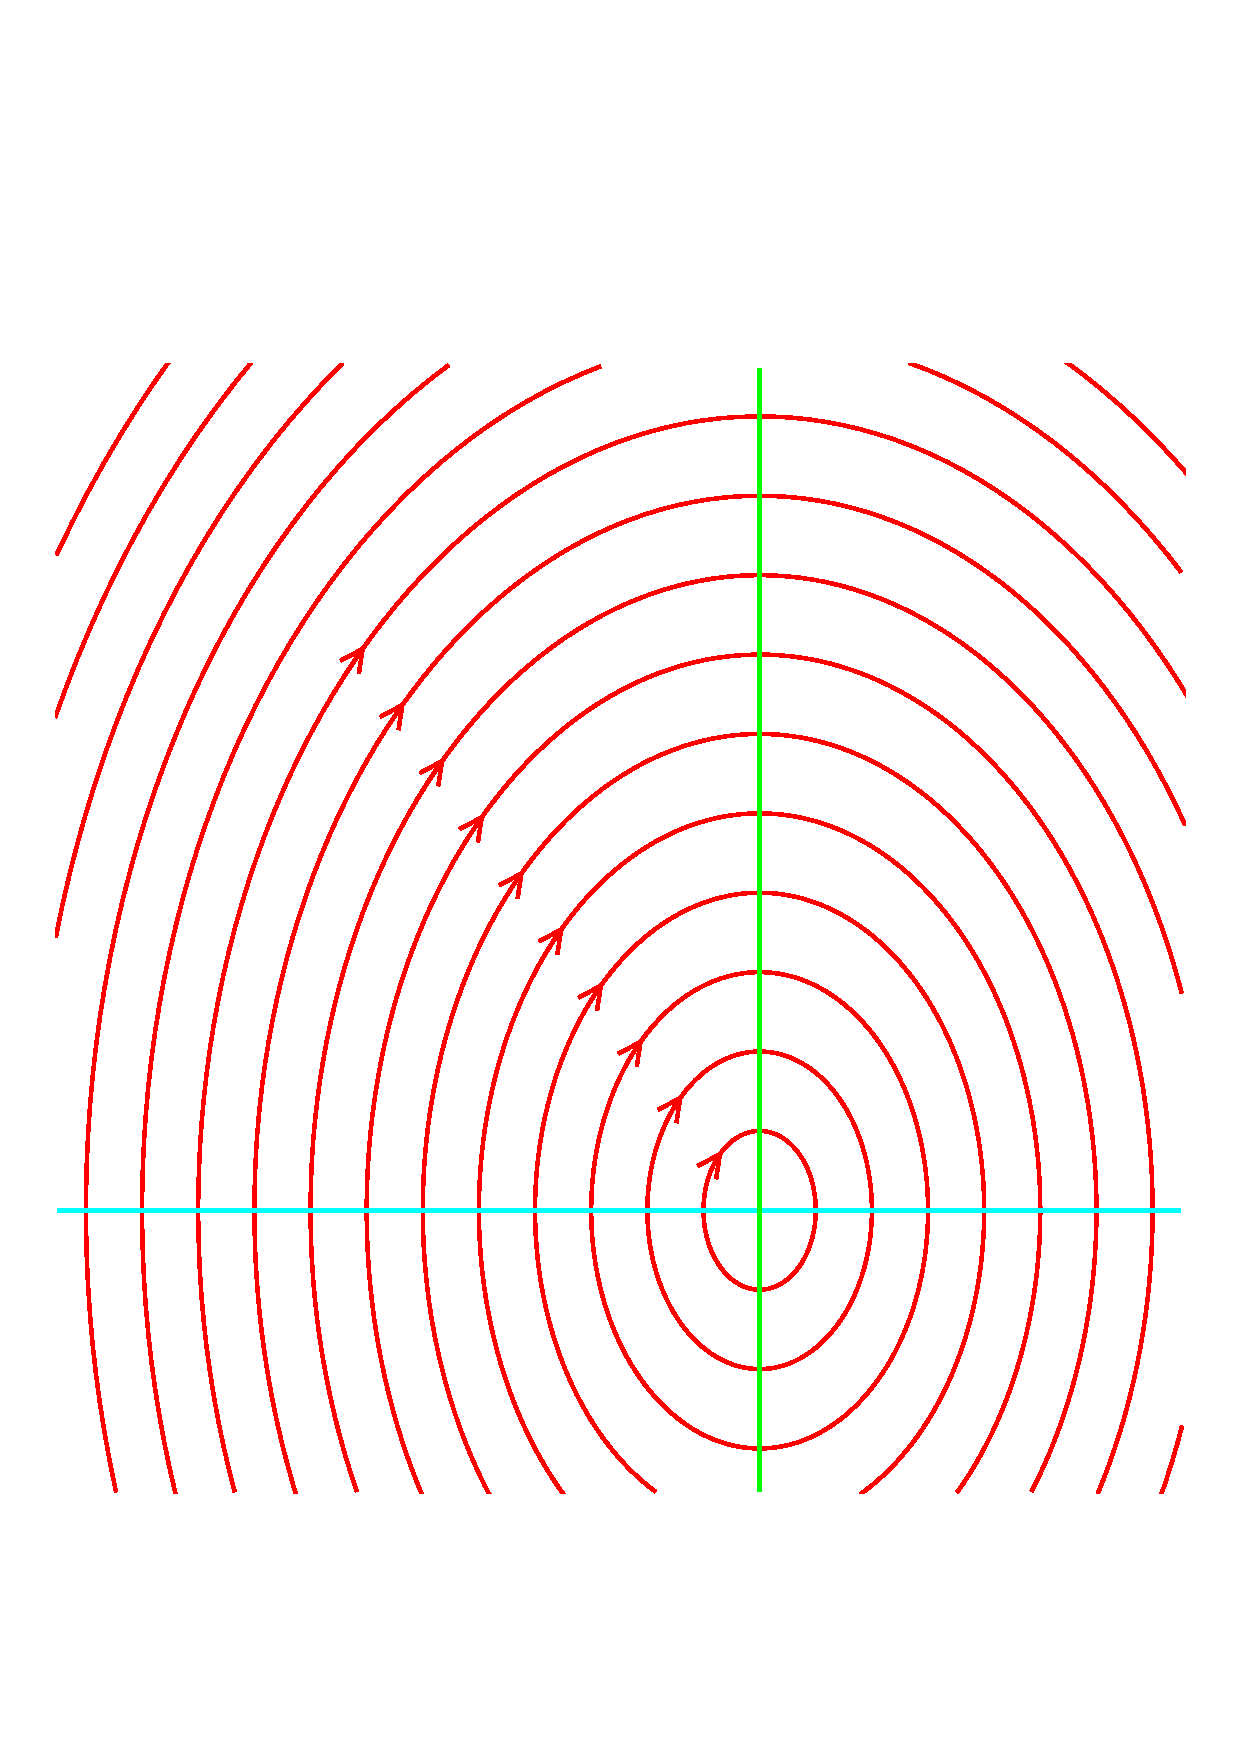
\includegraphics[scale=0.4]{../lectures/images/centre_offset.pdf} \]
\end{solution}

\begin{exercise}\label{ex-saddle-offset}
 Find and classify the equilibrium points for the system
 \begin{align*}
  \dot{x} &= f(x,y) = y-1 \\
  \dot{y} &= g(x,y) = x-1.
 \end{align*}
\end{exercise}
\begin{solution}
 For an equilibrium point, we need $y-1=x-1=0$.  Thus, there is a
 unique equilibrium point at $(1,1)$.  The Jacobian is
 $\left[\begin{array}{cc} 0 & 1 \\ 1 & 0 \end{array}\right]$, which
 has trace $\tau=0$ and determinant $\delta=-1$.  As $\delta<0$, this
 is a saddle.  In this case the functions $f$ and $g$ are just linear
 + constant, so there is no error in linearization, and the whole
 phase diagram is exactly the same as the usual phase diagram for a
 saddle, except that it has been shifted away from the origin.  The
 picture is as follows: 
 \[ 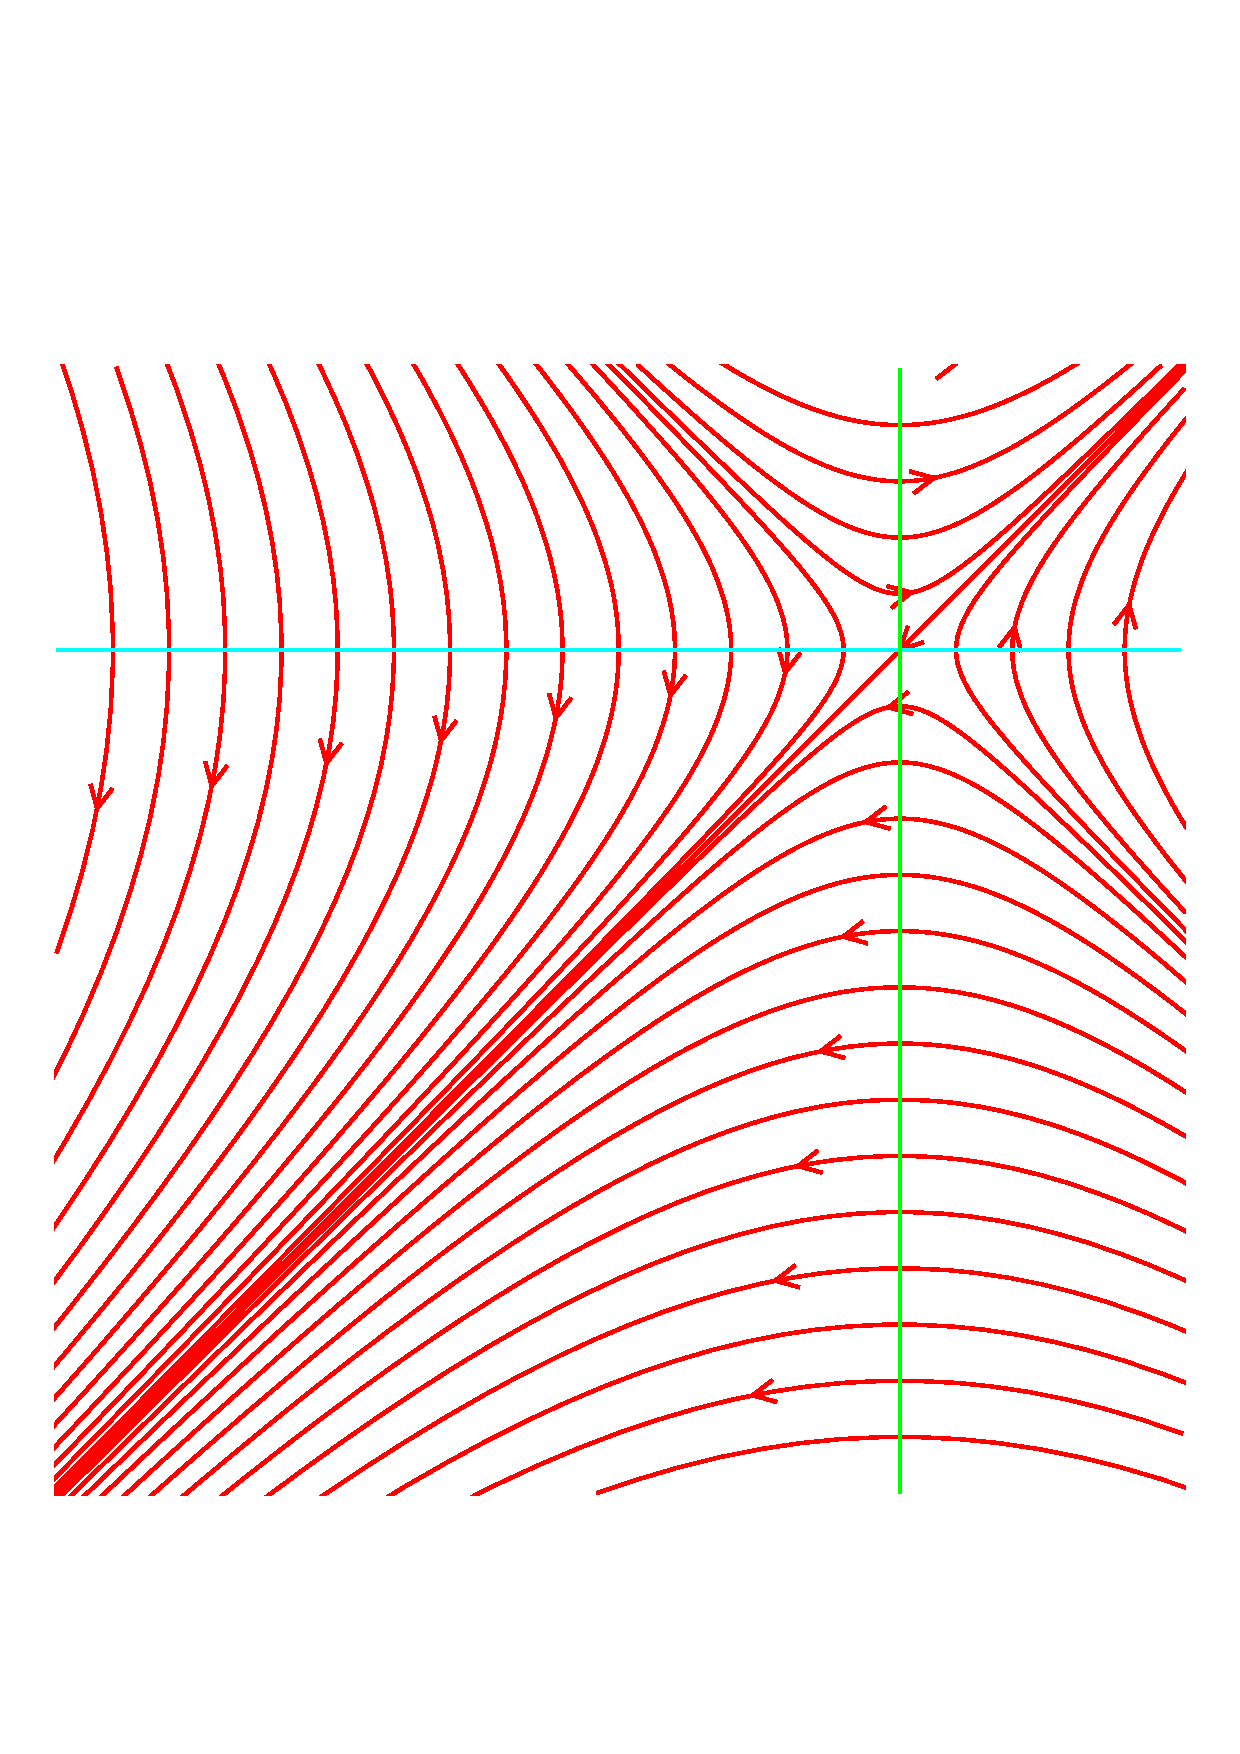
\includegraphics[scale=0.4]{../lectures/images/saddle_offset.pdf} \]
\end{solution}

\begin{exercise}\label{ex-quad-a}
 Find and classify the equilibrium points for the system 
 \begin{align*}
  \dot{x} &= f(x,y) = 25 - 16x^2 - 9y^2 \\
  \dot{y} &= g(x,y) = 9x^2 + 16y^2 - 25.
 \end{align*}
 Sketch the nullclines.
\end{exercise}
\begin{solution}
 If we divide the equation $\dot{x}=0$ by $16$ and divide the equation
 $\dot{y}=0$ by $9$ and add them together we get
 \[ \frac{25}{16} - x^2 - \frac{9}{16}y^2 + x^2 + \frac{16}{9}y^2 - \frac{25}{9}=0. \]
 This simplifies to
 $(\frac{16}{9}-\frac{9}{16})y^2=\frac{25}{9}-\frac{25}{16}$, but 
 $\frac{16}{9}-\frac{9}{16}=\frac{175}{144}=\frac{25}{9}-\frac{25}{16}$
 so we get $y^2=1$.  We can substitute $y^2=1$ in the equation
 $\dot{x}=25-16x^2-9y^2=0$ to get $16-16x^2=0$, so $x^2=1$ as well.
 We now see that $x=\pm 1$ and $y=\pm 1$, so there are four
 equilibrium points:
 \[ a_1 = (1,1) \qquad 
    a_2 = (-1,-1) \qquad
    a_3 = (1,-1) \qquad
    a_4 = (-1,1).
 \]
 To classify these, we use the Jacobian:
 \[ J = \left[\begin{array}{cc} \partial f/\partial x & \partial f/\partial y \\
             \partial g/\partial x & \partial g/\partial y \end{array}\right]
      = \bbm -32x & -18y \\ 18x & 32y \ebm.
 \]
 so the trace is $\tau=32(y-x)$ and the determinant is
 $\delta=(-32^2+18^2)xy=-700xy$.  We therefore have the following table:
 \[ \renewcommand\arraystretch{1.5} \begin{array}{|c|c|c|c|c|}
  \hline
                 & a_1  & a_2  & a_3  & a_4  \\ \hline
  \tau           &    0 &    0 &  -64 &   64 \\ \hline 
  \delta         & -700 & -700 &  700 &  700 \\ \hline
  \tau^2-4\delta & 2800 & 2800 & 1296 & 1296 \\ \hline
 \end{array} \]
 At $a_1$ and $a_2$ we have $\dl<0$, so these points are saddles.  At $a_2$ and
 $a_3$ we have $\tau^2-4\dl>0$, so these points are nodes.  At $a_2$ we have
 $\tau<0$, so this is a stable node.  At $a_3$ we have $\tau>0$, so this is an
 unstable node.  

 The $x$-nullcline has equation $16x^2+9y^2=25$, which describes an ellipse.  In
 more detail, we have $\frac{16}{25}x^2+\frac{9}{25}y^2=1$, or in other words 
 $(\frac{4}{5}x)^2+(\frac{3}{5}y)^2=1$.  This means that the point
 $(\frac{4}{5}x,\frac{3}{5}y)$ lies on the unit circle, so it is
 $(\cos(\tht),\sin(\tht))$ for some $\tht$.  This gives
 $x=\frac{5}{4}\cos(\tht)$ and $y=\frac{5}{3}\sin(\tht)$, which is an
 ellipse.  As $\frac{5}{3}>\frac{5}{4}$, the height of this ellipse is
 larger than the width.  Similarly, the $y$-nullcline is given by
 $9x^2+16y^2=25$, or
 $(x,y)=(\frac{5}{3}\cos(\tht),\frac{5}{4}\sin(\tht))$.  This is
 another ellipse, but in this case the width is larger than the
 height.  The phase portrait is as follows:
 \[ \includegraphics[scale=0.4]{../lectures/images/quad_a_xnyn.pdf} \]
\end{solution}

\begin{exercise}\label{ex-contour-flow}
 Consider the system
 \begin{align*}
  \dot{x} &= y^3-y = y(y+1)(y-1) \\
  \dot{y} &= x-x^3 = x(1+x)(1-x).
 \end{align*}
 \begin{itemize}
  \item[(a)] Show that the function $U=(x^2-1)^2/4+(y^2-1)^2/4$ is a
   conserved quantity.
  \item[(b)] Find and classify the equilibrium points.
 \end{itemize}
\end{exercise}
\begin{solution}\leavevmode
 \begin{itemize}
  \item[(a)] We have
   \begin{align*}
    U_x &= \frac{\partial U}{\partial x} =
             2(x^2-1)\tm 2x/4 = (x^2-1)x = x^3-x \\
    U_y &= \frac{\partial U}{\partial y} =
             2(y^2-1)\tm 2y/4 = (y^2-1)y = y^3-y \\
    \dot{U} &= U_xf + U_yg = (x^3-x)(y^3-y) + (y^3-y)(x-x^3) = 0.
   \end{align*}
   Thus, $U$ is conserved.
  \item[(b)] 
   The $x$-nullcline consists of three horizontal lines, with equations
   $y=0$, $y=1$ and $y=-1$.  Similarly, the $y$-nullcline consists of
   three vertical lines, with equations $x=0$, $x=1$ and $x=-1$.  This
   means that there are nine equilibrium points $(n,m)$ with
   $n,m\in\{-1,0,1\}$.  The Jacobian is
   \[ J = \left[\begin{array}{cc} \partial f/\partial x & \partial f/\partial y \\
               \partial g/\partial x & \partial g/\partial y \end{array}\right]
        = \left[\begin{array}{cc} 0 & 3y^2-1 \\
               1-3x^2 & 0 \end{array}\right],
   \]
   so the trace is $\tau=0$ and the determinant is
   $\delta=(1-3x^2)(1-3y^2)$.  As $\tau=0$ we see that the equilibrium
   points are centres if $\delta>0$, and saddles if $\delta<0$.  If $x$ and
   $y$ are both zero then $\delta=1$, corresponding to a centre.  We
   have seen other examples where the linearised system has a centre
   but the original nonlinear system has a slow spiral.  However, that
   cannot  happen here because we have a conserved quantity, which
   forces the flow lines to close up as circles.  The bottom
   left entry in $J$ is $1-3x^2=1>0$, so the rotation is anticlockwise.
   If $x=0$ and $y=\pm 1$ then $\delta=-2<0$, corresponding to a saddle.
   The same applies if $x=\pm 1$ and $y=0$.  Finally, if both $x$ and
   $y$ are $\pm 1$ then $\delta>0$, which means we have another centre.  The
   bottom left entry is $-2<0$, so the rotation is clockwise.
 \end{itemize}

 The phase portrait for this system was shown in lectures:
 \[ 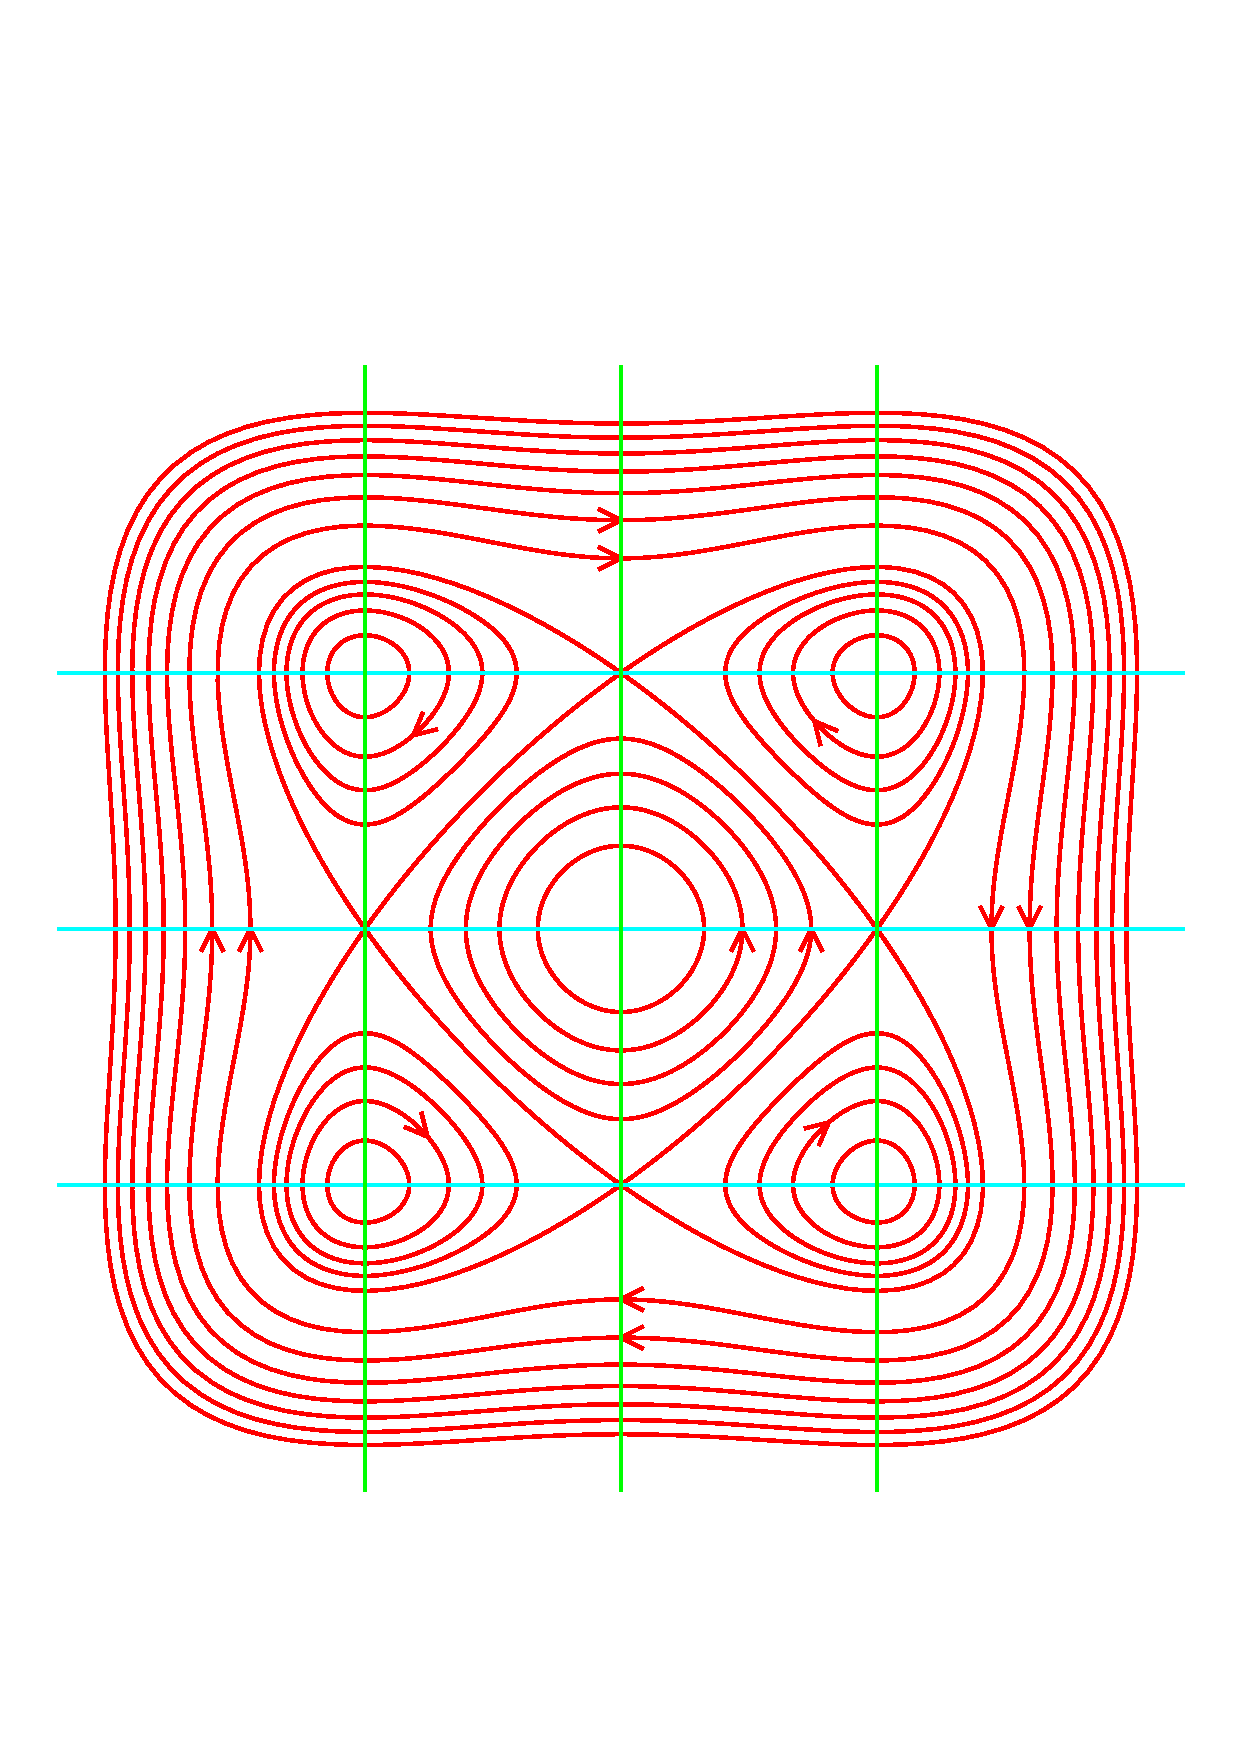
\includegraphics[scale=0.4]{../lectures/images/contour_flow_xnyn.pdf} \]
\end{solution}

\begin{exercise}\label{ex-doubly-periodic}
 Consider the system
 \begin{align*}
  \dot{x} &= f(x,y) = \sin(\pi y) \\
  \dot{y} &= g(x,y) = \sin(\pi x).
 \end{align*} 
 \begin{itemize}
  \item[(a)] Show that the function $U=\cos(\pi x)-\cos(\pi y)$ is a
   conserved quantity.
  \item[(b)] Find and classify the equilibrium points.
  \item[(c)] Sketch the phase portrait.
 \end{itemize}
\end{exercise}
\begin{solution}\leavevmode
 \begin{itemize}
  \item[(a)] We have
   \[ \dot{U} = U_xf+U_yg =
       -\pi\sin(\pi x).\sin(\pi y) +\pi\sin(\pi y)\sin(\pi x) = 0,
   \]
   so $U$ is conserved.
  \item[(b)] The $x$-nullcline is given by $\sin(\pi y)=0$, which
   means that $y$ must be an integer.  Similarly, the $y$-nullcline is
   given by $\sin(\pi x)=0$, which means that $x$ must be an integer.
   Thus, the equilibrium points are of the form $(n,m)$, where $n$ and
   $m$ are both integers.  The Jacobian is 
   \[ J = \left[\begin{array}{cc} \partial f/\partial x & \partial f/\partial y \\
               \partial g/\partial x & \partial g/\partial y \end{array}\right]
        = \left[\begin{array}{cc} 0 & \pi\cos(\pi y) \\ \pi\cos(\pi x) & 0 \end{array}\right],
   \]
   so the trace is $\tau=0$ and the determinant is
   $\delta=-\pi^2\cos(\pi x)\cos(\pi y)$.  At an equilibrium point
   $(n,m)$ we have $\cos(\pi x)=(-1)^n$ and $\cos(\pi y)=(-1)^m$, so
   $\delta=(-1)^{n+m+1}\pi^2$.  If $n$ and $m$ are both odd, or both
   even, then we have $\delta=-\pi^2<0$, so $(n,m)$ is a saddle.  If
   $n$ is odd and $m$ is even then $\delta=\pi^2>0$ and $\tau=0$ so we
   have a centre, at least for the linearised system.  We have seen
   other examples where the linearised system has a centre but the
   original nonlinear system has a slow spiral.  However, that cannot
   happen here because we have a conserved quantity, which forces the
   flow lines to close up as circles.  The bottom left
   entry in $J$ is $\cos(\pi x)=(-1)^n=-1$, so the rotation is
   clockwise.  Similarly, if $n$ is even and $m$ is odd then we again
   have a centre, but in this case the rotation is anticlockwise. 
  \item[(c)] The phase portrait is as follows:
   \[ 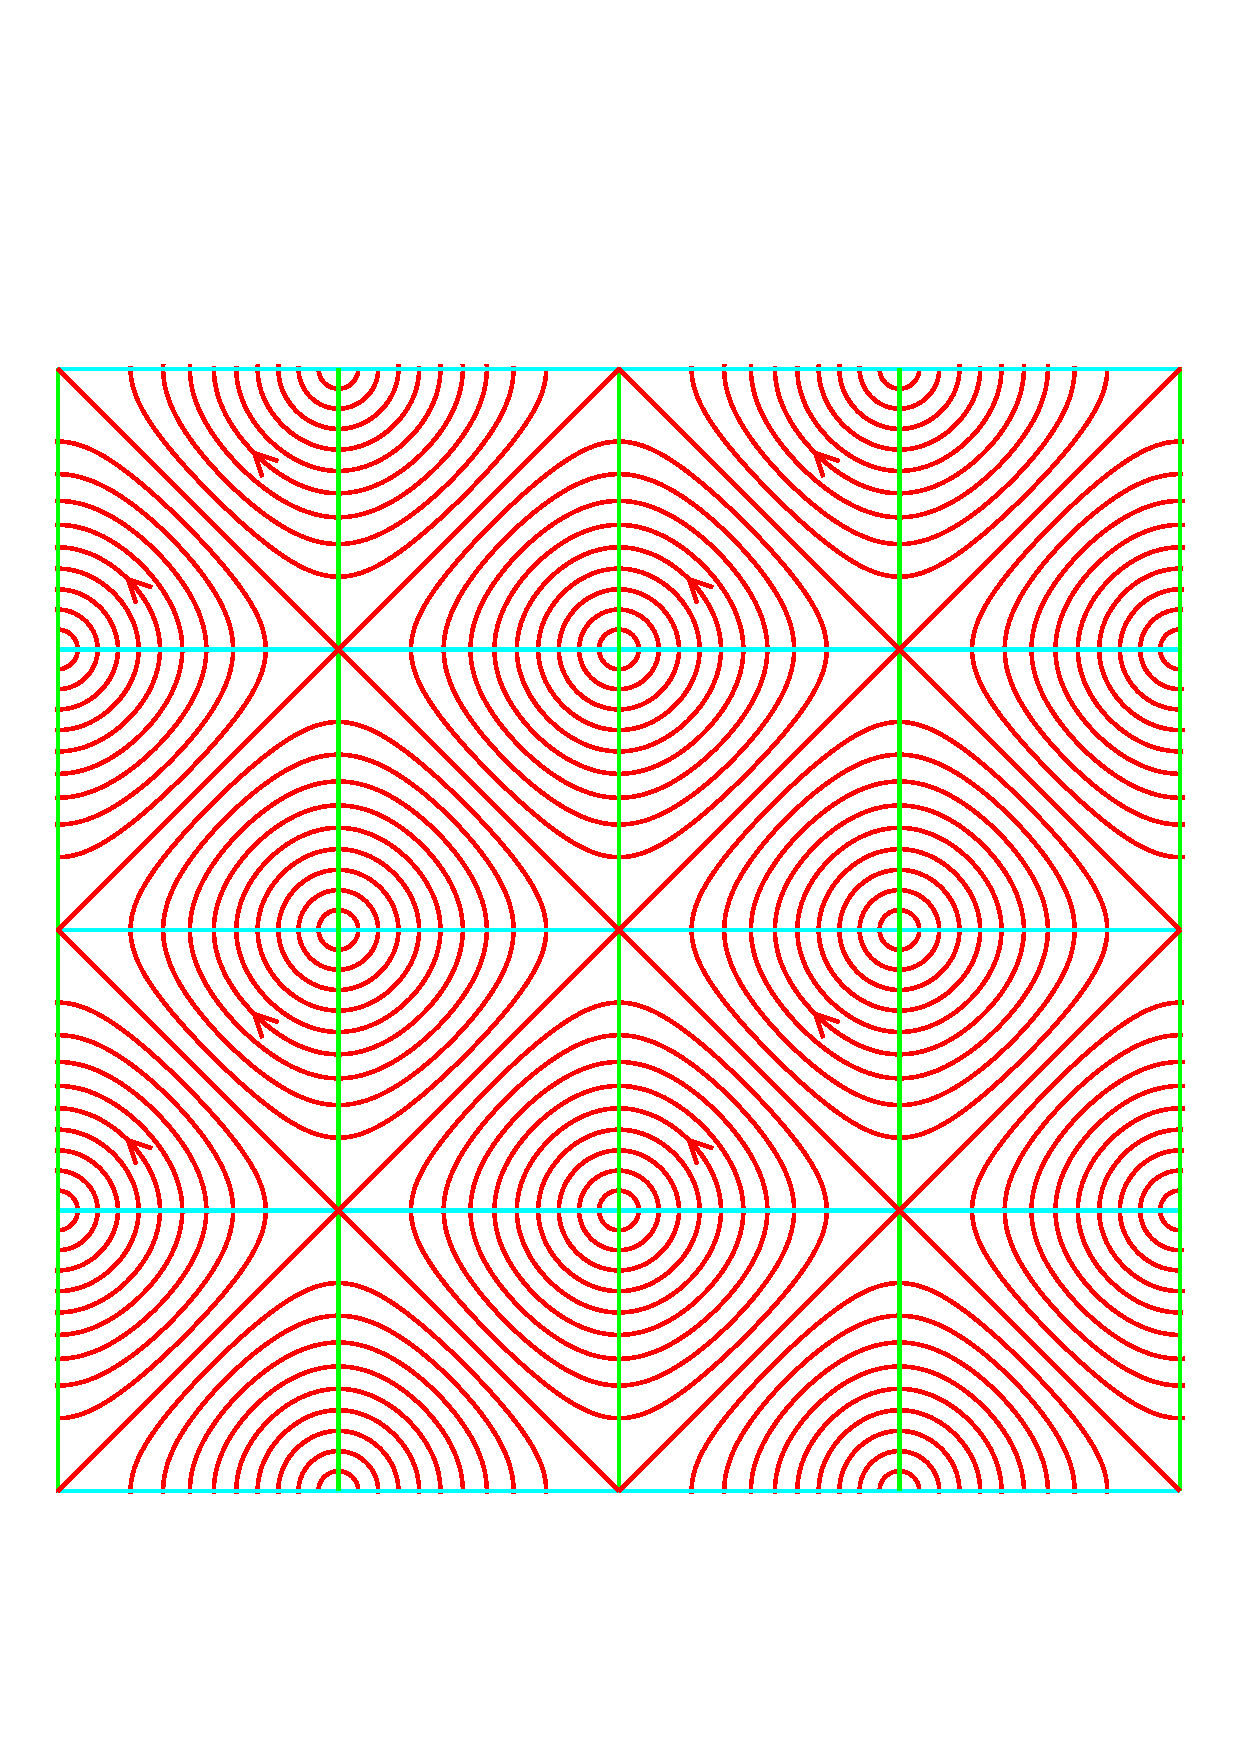
\includegraphics[scale=0.4]{../lectures/images/doubly_periodic.pdf} \]
 \end{itemize}
\end{solution}

\begin{exercise}\label{ex-phase-sketch}
 Sketch the phase portrait of the system $\dot{x}=y$,
 $\dot{y}=-x-x^2-y$ in a neighbourhood of the origin.
\end{exercise}
\begin{solution}

 \[ 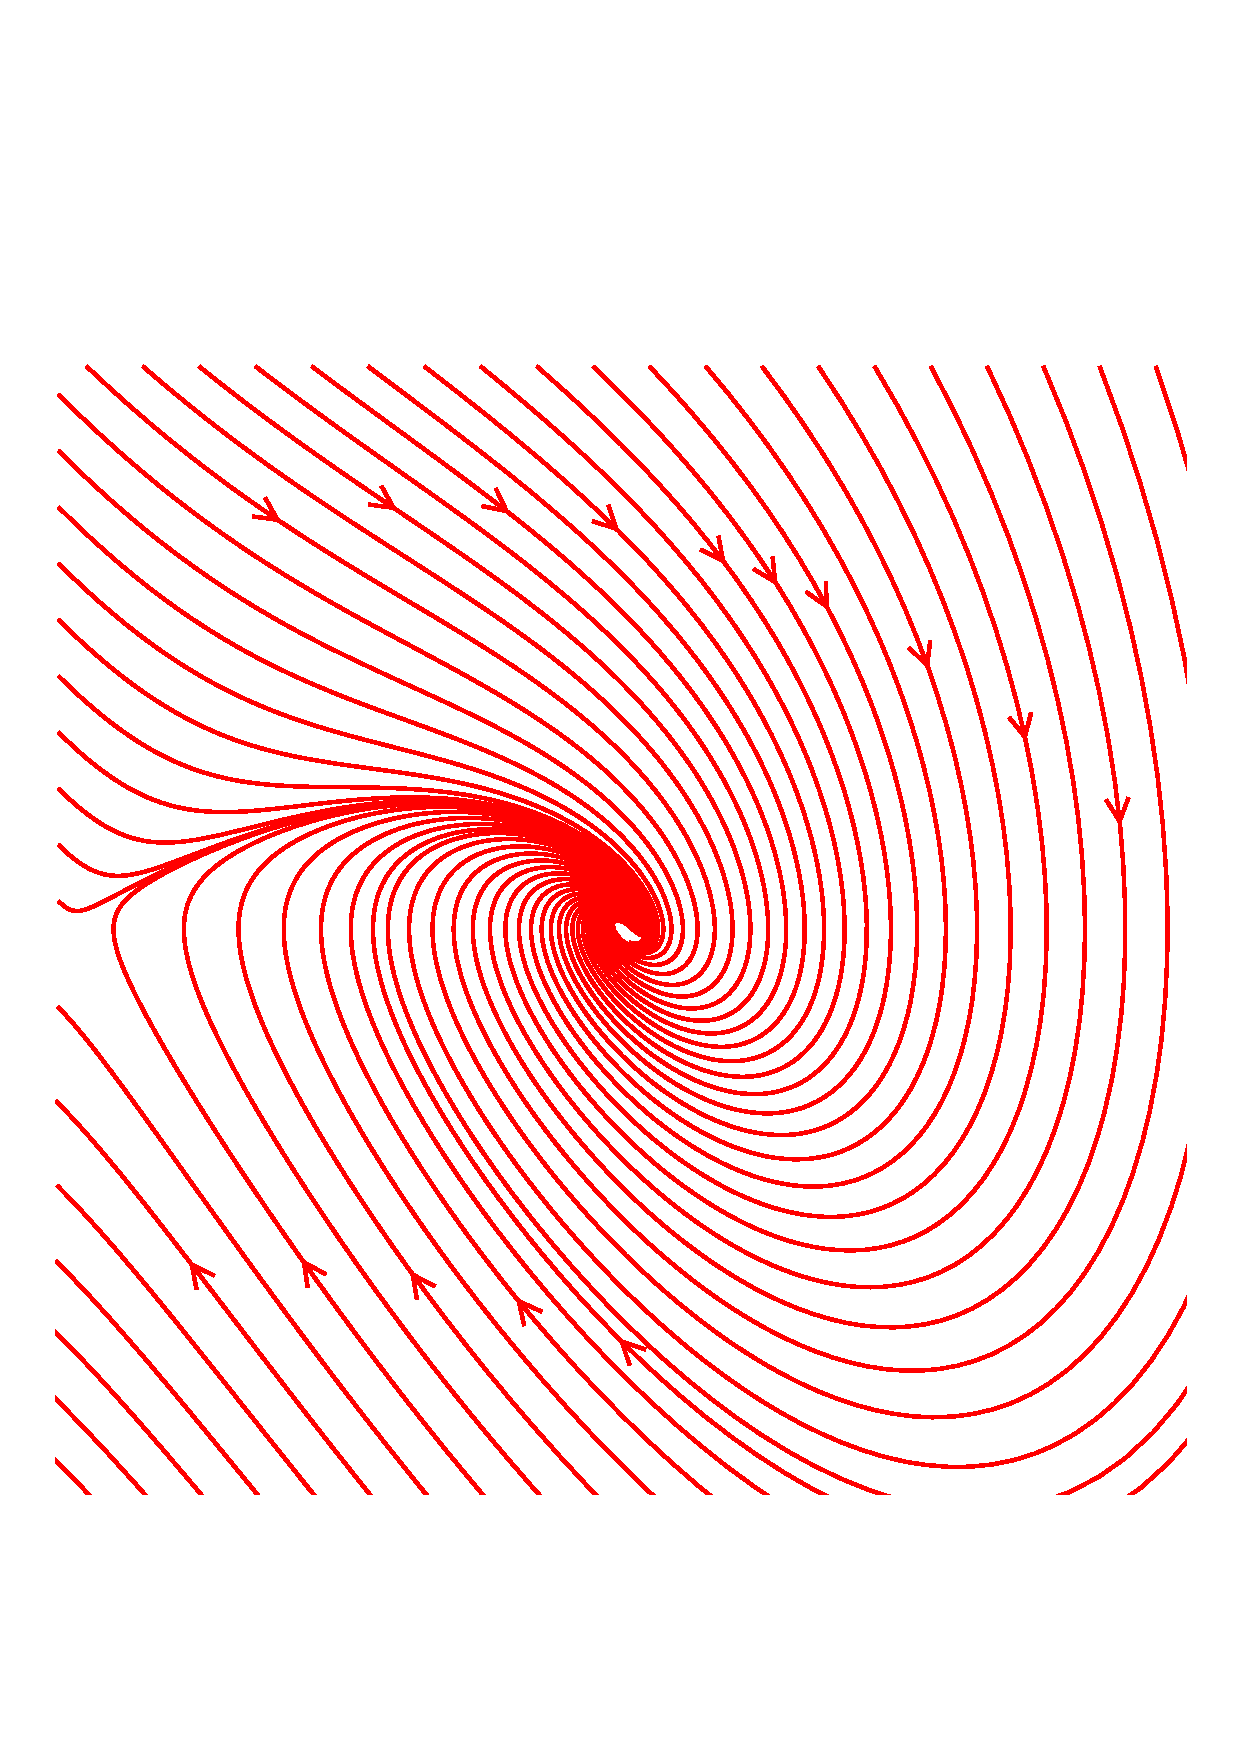
\includegraphics[scale=0.4]{../lectures/images/misc_f.pdf} \]
\end{solution}

\begin{exercise}\label{ex-general-quadratic}
 Let $a,b,c,d,p$ and $q$ be constants with $a\neq 0$ and $d\neq 0$ and
 $ad-bc\neq 0$.  Consider the system 
 \begin{align*}
  \dot{x} &= f(x,y) = x(ax+by-p) \\
  \dot{y} &= g(x,y) = y(cx+dy-q).
 \end{align*}
 Find the four equilibrium points, and give a formula for the Jacobian
 matrix at each of these points.
\end{exercise}
\begin{solution}
 For an equilibrium point, we must have either $x=0$ or $ax+by=p$, and
 also $y=0$ or $cx+dy=q$.  If $x=0$ then the equation $cx+dy=q$
 becomes $y=q/d$, and if $y=0$ then the equation $ax+by=p$ becomes
 $x=p/a$.  If $x$ and $y$ are both nonzero then we must have $ax+by=p$
 and $cx+dy=q$.  If we multiply the first equation by $d$ and the
 second equation by $b$ and subtract, we get $(ad-bc)x=dp-bq$, so 
 $x=\frac{dp-bq}{ad-bc}$.  Similarly, we can multiply the first
 equation by $c$ and the second equation by $a$ and subtract to get
 $(bc-ad)y=cp-aq$, so $y=\frac{aq-cp}{ad-bc}$.  We thus have
 four equilibrium points:
 \[ a_1 = \left[\begin{array}{cc} 0\\ 0\end{array}\right] \qquad
    a_2 = \left[\begin{array}{cc} 0\\ q/d\end{array}\right] \qquad
    a_3 = \left[\begin{array}{cc} p/a\\ 0\end{array}\right] \qquad
    a_4 = \frac{1}{ad-bc}\left[\begin{array}{cc} dp-bq \\ aq-cp \end{array}\right].
 \]
 The Jacobian matrix is 
 \[ J = \left[\begin{array}{cc} \partial f/\partial x & \partial f/\partial y \\
             \partial g/\partial x & \partial g/\partial y \end{array}\right]
      = \left[\begin{array}{cc} 2ax+by-p & bx \\
             cy & cx+2dy-q \end{array}\right].
 \]
 Evaluating this at the equilibrium points $a_1,\dotsc,a_4$ gives
 \[ J_1 = \left[\begin{array}{cc} -p & 0 \\ 0 & -q \end{array}\right] \qquad
    J_2 = \left[\begin{array}{cc} (bq-dp)/d & 0 \\ cq/d & q \end{array}\right] \qquad
    J_3 = \left[\begin{array}{cc} p & bp/a \\ 0 & (cp-aq)/a \end{array}\right]
 \]
 and
 \[ J_4 = \frac{1}{ad-bc} \left[\begin{array}{cc} a(dp-bq) & b(dp-bq) \\
                               c(aq-cp) & d(aq-cp) \end{array}\right].
 \]
\end{solution}

\begin{exercise}\label{ex-gradient-flow}
 In lectures we considered the system
 \[ \dot{x} = x-x^3 \hspace{4em} \dot{y} = y-y^3. \]
 Suppose that $x_0,y_0>0$.  Show that the formulae
 \[ x = (1+(x_0^{-2}-1)e^{-2t})^{-1/2} \hspace{4em}
    y = (1+(y_0^{-2}-1)e^{-2t})^{-1/2}
 \]
 give an explicit solution for this system, with $(x,y)=(x_0,y_0)$ at
 $t=0$. 
\end{exercise}
\begin{solution}
 It will be convenient to put $C=x_0^{-2}-1$, so
 $x=(1+Ce^{-2t})^{-1/2}$.  This gives 
 \begin{align*}
  \dot{x} &= -\half(1+Ce^{-2t})^{-3/2}\tm(-2)\tm
              Ce^{-2t} 
           = (1+Ce^{-2t})^{-3/2}C e^{-2t} \\
  x-x^3 &= x^3(x^{-2}-1)
         = (1+Ce^{-2t})^{-3/2}(1+Ce^{-2t}-1) 
         = (1+Ce^{-2t})^{-3/2}C e^{-2t} = \dot{x},
 \end{align*}
 as required.  Also, at $t=0$ we have $e^{-2t}=1$ so
 $x=(1+C)^{-1/2}=(x_0^{-2})^{-1/2}=x_0$.  Essentially the same
 argument gives $\dot{y}=y-y^3$ and $y=y_0$ at $t=0$.
\end{solution}

\begin{exercise}\label{ex-xy}
 Consider the system $\dot{x}=\dot{y}=xy$. 
 \begin{itemize}
  \item[(a)] Find a conserved quantity.  (There is a very simple one.)
  \item[(b)] Show that for any $x_0,y_0>0$ we have a solution 
   \[ x = \frac{x_0(x_0-y_0)}{x_0-y_0e^{t(x_0-y_0)}} 
      \hspace{5em}
      y = \frac{y_0(y_0-x_0)}{y_0-x_0e^{t(y_0-x_0)}}. 
   \]
  \item[(c)] Check that the solution in~(b) becomes infinite when 
   $t=(\ln(x_0)-\ln(y_0))/(x_0-y_0)$.
  \item[(d)] What is the value of the conserved quantity on the
   solution in~(b)?
 \end{itemize}
\end{exercise}
\begin{solution}
 \begin{itemize}
  \item[(a)] As $\dot{x}=\dot{y}$ we see that the function $U=x-y$ has
   $\dot{U}=0$, so $U$ is a conserved quantity.
  \item[(b)] It will be convenient to put $a=x_0-y_0$ and $u=e^{at}$.
   In terms of these, we have 
   \[ x = \frac{x_0a}{x_0-y_0u} \hspace{5em}
      y = \frac{-y_0a}{y_0-x_0/u} 
        = \frac{y_0au}{x_0-y_0u}.
   \]
   Note also that $a$ is constant and $\dot{u}=ae^{at}=au$.  This
   gives
   \[ \dot{x} =
       -\frac{x_0a}{(x_0-y_0u)^2}(-y_0\dot{u}) = 
       -\frac{x_0a}{(x_0-y_0u)^2}(-y_0au) = 
        \frac{x_0y_0a^2u}{(x_0-y_0u)^2} = xy.
   \]
   A similar argument also gives $\dot{y}=xy$.
  \item[(c)] Put $t^*=(\ln(x_0)-\ln(y_0))/(x_0-y_0)$.  We then have
   $at^*=\ln(x_0)-\ln(y_0)=\ln(x_0/y_0)$, so when $t=t^*$ we have
   $u=e^{at^*}=x_0/y_0$.  This means that the denominator $x_0-y_0u$
   is zero, so the solution goes to infinity.
  \item[(d)] At $t=0$ we have $u=1$ and so $x=x_0$ and $y=y_0$ and
   $U=x-y=x_0-y_0$.  As $U$ is conserved, we must have $U=x_0-y_0$ for
   all $t$.  This can also be seen explicitly:
   \[ U = x-y = \frac{x_0a}{x_0-y_0u} - \frac{y_0au}{x_0-y_0u}
         = \frac{(x_0-y_0u)a}{x_0-y_0u} = a = x_0-y_0.
   \] 
 \end{itemize}
\end{solution}

\begin{exercise}\label{ex-complex-square-b}
 Consider the system
 \[ \dot{x} = x^2-y^2 \hspace{4em} \dot{y} = 2xy. \]
 \begin{itemize}
  \item[(a)] Show that the origin is the only equilibrium point, and
   that the Jacobian is zero at the origin.
  \item[(b)] Show that the formulae
   \begin{align*}
    A &= x_0^2 + y_0^2 \\
    u &= x_0 - tA & v &= 1 - 2tx_0 + t^2A \\
    x &= u/v & y &= y_0/v
   \end{align*}
   give an explicit solution with $(x,y)=(x_0,y_0)$ when $t=0$.
  \item[(c)] Let $R$ be a large positive number.  Show that the
   solution starting at $(R^3/(R^4+1),\;R/(R^4+1))$ (very close to the
   origin) reaches the point $(0,R)$ (very far from the origin) at
   $t=R$.  This shows that the origin is unstable.
 \end{itemize}
\end{exercise}
\begin{solution}\leavevmode
 \begin{itemize}
  \item[(a)] At an equilibrium point we must have $x^2-y^2=0$ (so
   $x=\pm y$) and $2xy=0$ (so either $x$ or $y$ is zero).  The only
   way to satisfy both conditions is if $x=y=0$, so the origin is the
   only equilibrium point.  The Jacobian is 
   \[ J=\left[\begin{array}{cc} 2x&-2y\\ 2y&2x\end{array}\right], \]
   which becomes zero when $x=y=0$.
  \item[(b)] First note that when $t=0$ we have $u=x_0$ and $v=1$ so
   $x=u/v=x_0$ and $y=y_0/v=y_0$ as expected.  We also have
   \begin{align*}
    \dot{u} &= -A \\
    \dot{v} &= -2x_0 +2tA \\
    \dot{x} &= \frac{\dot{u}v-u\dot{v}}{v^2} 
             = (-A(1-2tx_0+t^2A^2)-(x_0-tA)(-2x_0+2tA))/v^2 \\
            &= (-A+2tAx_0-t^2A^3+x_0^2-2tAx_0-2tAx_0+2t^2A^2)/v^2 \\
            &= (-A+2x_0^2-2tAx_0+t^2A^2)/v^2 \\
            &= (x_0^2-y_0^2-2tAx_0+t^2A^2)/v^2 \\
    \dot{y} &= -\frac{y_0\dot{v}}{v^2} = 2y_0(x_0-tA)/v^2 \\
    x^2-y^2 &= \frac{u^2-y_0^2}{v^2} \\
            &= (x_0^2-2tAx_0+t^2A^2-y_0^2)/v^2 \\
    2xy     &= 2uy_0/v^2 = 2(x_0-tA)y_0/v^2.
   \end{align*}
   From this it is clear that $\dot{x}=x^2-y^2$ and $\dot{y}=2xy$, as
   required.
  \item[(c)] Now take $x_0=R^3/(R^4+1)$ and $y_0=R/(R^4+1)$ and
   $t=R$.  This gives 
   \begin{align*}
    A &= x_0^2+y_0^2 = \frac{R^6+R^2}{(R^4+1)^2} = \frac{R^2(R^4+1)}{(R^4+1)^2} = \frac{R^2}{R^4+1} \\
    u &= x_0-tA = \frac{R^3}{R^4+1} - R\frac{R^2}{R^4+1} = 0 \\
    v &= 1-2tx_0+t^2A = 1 - 2R\frac{R^3}{R^4+1} + R^2\frac{R^2}{R^4+1}
       = 1 - \frac{R^4}{R^4+1} = \frac{1}{R^4+1} \\
    x &= u/v = 0 \\
    y &= y_0/v = \frac{R}{R^4+1}/\frac{1}{R^4+1} = R.
   \end{align*}
 \end{itemize}
\end{solution}

\begin{exercise}\label{ex-complex-square-offset}
 Consider the system 
 \begin{align*}
  \dot{x} &= f(x,y) = x^2-y^2-1/4 \\
  \dot{y} &= g(x,y) = 2xy.
 \end{align*}
 \begin{itemize}
  \item[(a)] Show that the $x$-nullcline consists of all points of the
   form $(\pm\cosh(s)/2,\sinh(s)/2)$.
  \item[(b)] Find the $y$-nullcline.
  \item[(c)] Find and classify the equilibrium points.
  \item[(d)] Sketch the phase portrait.
 \end{itemize}
\end{exercise}
\begin{solution}\leavevmode
 \begin{itemize}
  \item[(a)] If $(x,y)$ lies on the $x$-nullcline we must have
   $x^2-y^2-1/4=0$, which can be rearranged as $(2x-2y)(2x+2y)=1$.
   Put $u=2x+2y$ so $u^{-1}=2x-2y$.  Adding these equations gives
   $x=(u+u^{-1})/4$, and subtracting them gives $y=(u-u^{-1})/4$.  If
   $u>0$ we can put $s=\ln(u)$ and we find that
   $x=(e^s+e^{-s})/4=\cosh(s)/2$ and $y=(e^s-e^{-s})/4=\sinh(s)/2$.
   On the other hand, if $u<0$ we can put $s=-\ln(-u)$ and we find that 
   $x=(-e^{-s}-e^s)/4=-\cosh(s)/2$ and $y=(-e^{-s}+e^s)/4=\sinh(s)/2$.
  \item[(b)] The $y$-nullcline is given by $2xy=0$, so $x=0$ or $y=0$.
  \item[(c)] At an equilibrium point, we must have $x^2-y^2-1/4=0$ and
   also $xy=0$, so either $x=0$ or $y=0$.  If $x=0$ then the equation
   $x^2-y^2-1/4=0$ becomes $y^2+1/4=0$, which is impossible because
   $y^2\geq 0$.  If $y=0$ then the equation $x^2-y^2-1/4=0$ becomes
   $x^2-1/4=0$, which gives $x=\pm\half$.  Thus, the equilibrium
   points are $a_1=(-1/2,0)$ and $a_2=(1/2,0)$.  

   The Jacobian is
   $J=\left[\begin{array}{cc} 2x&-2y\\ 2y&2x\end{array}\right]$, which
   is $-I$ at $a_1$ and $+I$ at $a_2$.  This means that $a_1$ is an
   improper stable node and $a_2$ is an improper unstable node.
  \item[(d)] The phase portrait is as follows:
   \[ 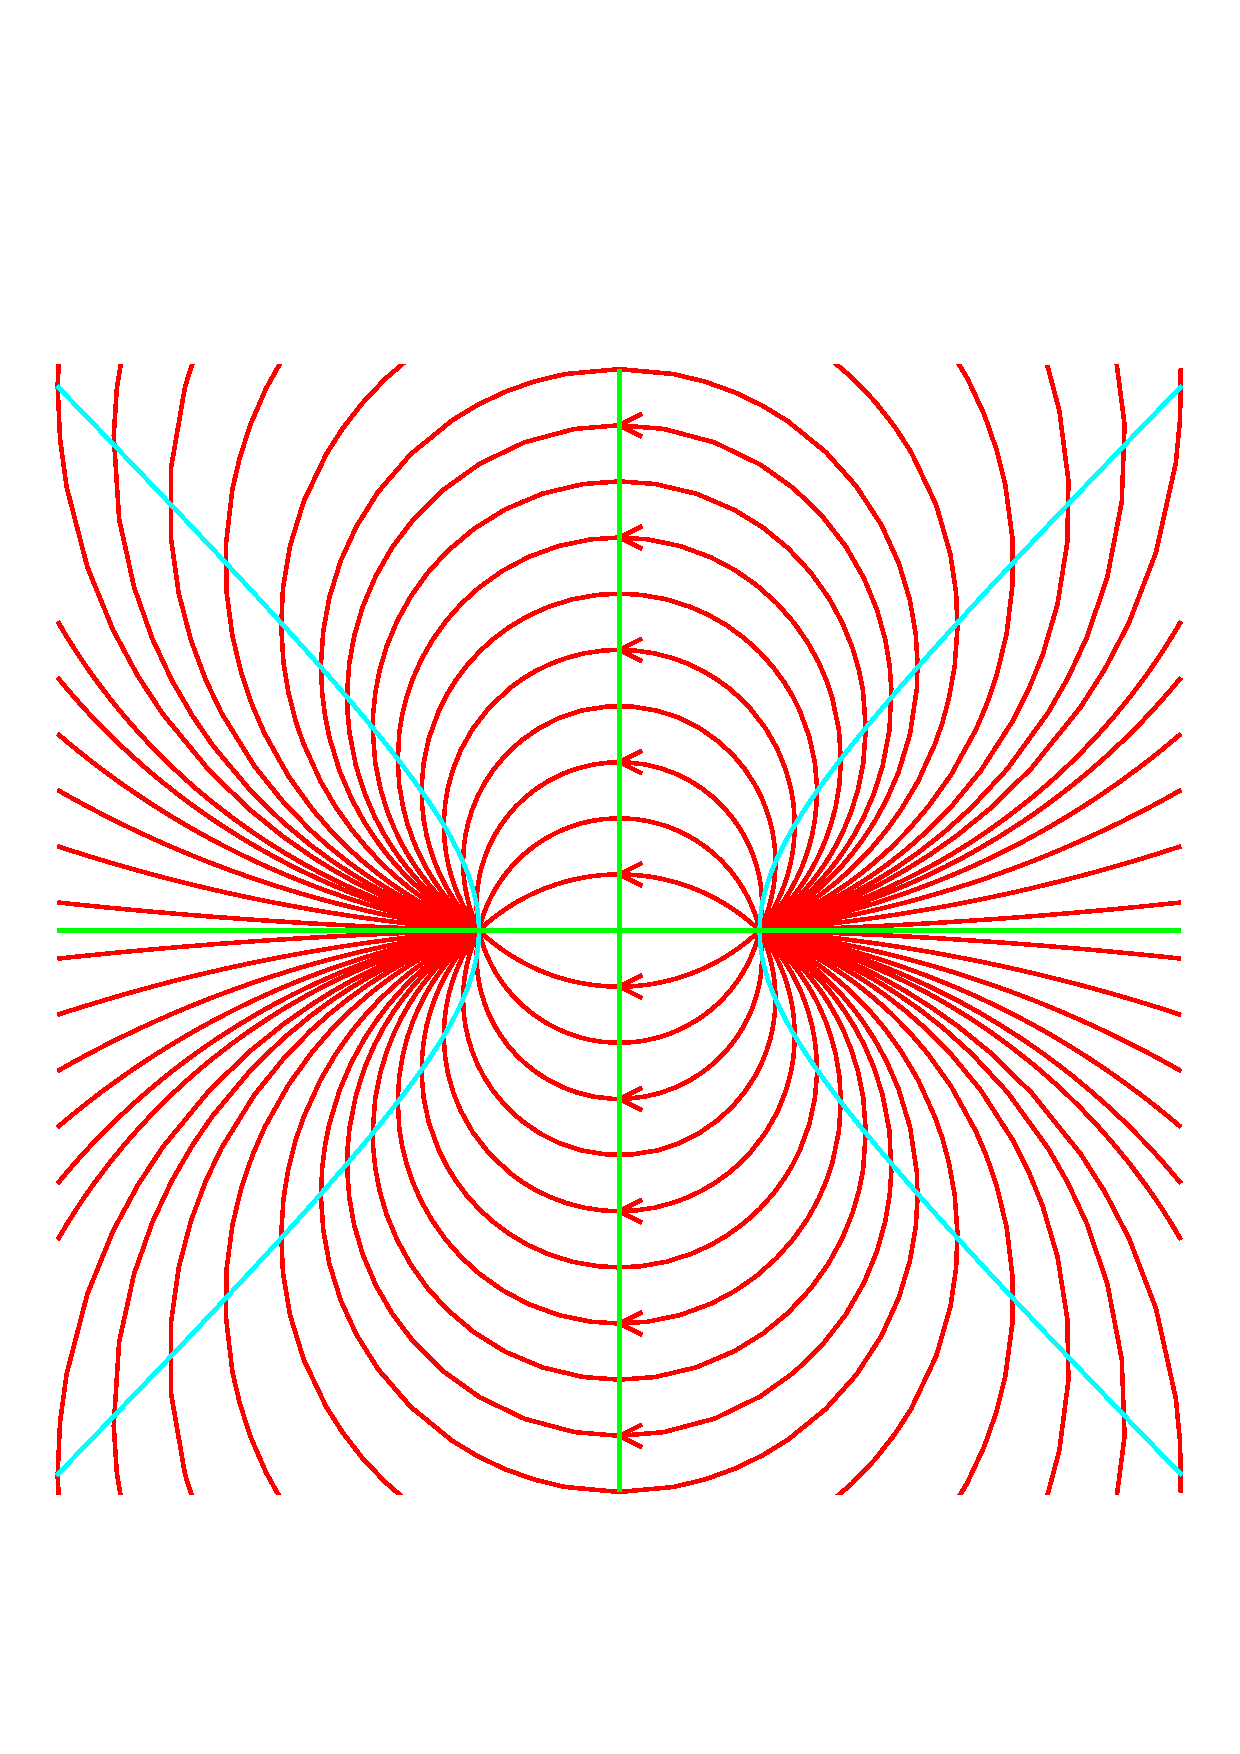
\includegraphics[scale=0.4]{../lectures/images/complex_square_offset.pdf} \]
 \end{itemize}
\end{solution}

\begin{exercise}\label{ex-fluid}
 The system 
 \[ \dot{x} = x^2-y^2+2xy \hspace{4em} \dot{y} = x^2-y^2-2xy \]
 has some solutions of the form $(x,y)=(a/t,b/t)$.  Find the relevant
 values of $a$ and $b$.
\end{exercise}
\begin{solution}
 If $x=a/t$ and $y=b/t$ then 
 \begin{align*}
  \dot{x} &= -a/t^2 \\
  \dot{y} &= -b/t^2 \\
  x^2-y^2+2xy &= (a^2-b^2+2ab)/t^2 \\
  x^2-y^2-2xy &= (a^2-b^2-2ab)/t^2.
 \end{align*}
 Thus, we have a solution to the given system if
 \begin{align*}
  -a &= a^2-b^2+2ab \tag{A} \\
  -b &= a^2-b^2-2ab. \tag{B}
 \end{align*}
 If we add and subtract these equations, we get
 \begin{align*}
  -a-b &= 2(a^2-b^2) = 2(a+b)(a-b) \tag{C} \\
   b-a &= 4ab. \tag{D}
 \end{align*}
 Equation~(C) can be rearranged as $(a+b)(2a-2b+1)=0$, so either
 $b=-a$ or $b=a+\half$.  
 \begin{itemize}
  \item[(a)] If $b=-a$ then equation~(D) becomes $-2a=-4a^2$, so
   $2a^2=a$, so $a(1-2a)=0$, so $a=0$ or $a=\half$.  If $a=0$ then
   $b=0$, and if $a=\half$ then $b=-\half$.  We thus have two
   solutions to the original system: the constant solution
   $(x,y)=(0,0)$, and the solution $(x,y)=(1/(2t),-1/(2t))$.
  \item[(b)] Suppose instead that $b=a+\half$.  Then equation~(D)
   becomes $\half=4a(a+\half)$, and this can be rearranged as
   $4a^2+2a-\half=0$, or $a^2+\half a-\tfrac{1}{8}=0$.  This has
   solutions 
   \[ a = (-\half\pm\sqrt{\tfrac{1}{4}+\half})/2 = 
        (-1\pm\sqrt{3})/4.
   \]
   The corresponding values of $b=a+\half$ are $(+1\pm\sqrt{3})/4$.
   We therefore have two solutions to the original system:
   \[
    (x,y) =
     \left(\frac{-1+\sqrt{3}}{4t},\frac{1+\sqrt{3}}{4t}\right)
    \qquad \text{ or } \qquad
    (x,y) =
     \left(\frac{-1-\sqrt{3}}{4t},\frac{1-\sqrt{3}}{4t}\right).
   \]
 \end{itemize}
 In the following picture, the above solutions are the straight blue
 lines.  Some other flow lines are shown in red.

 \[ 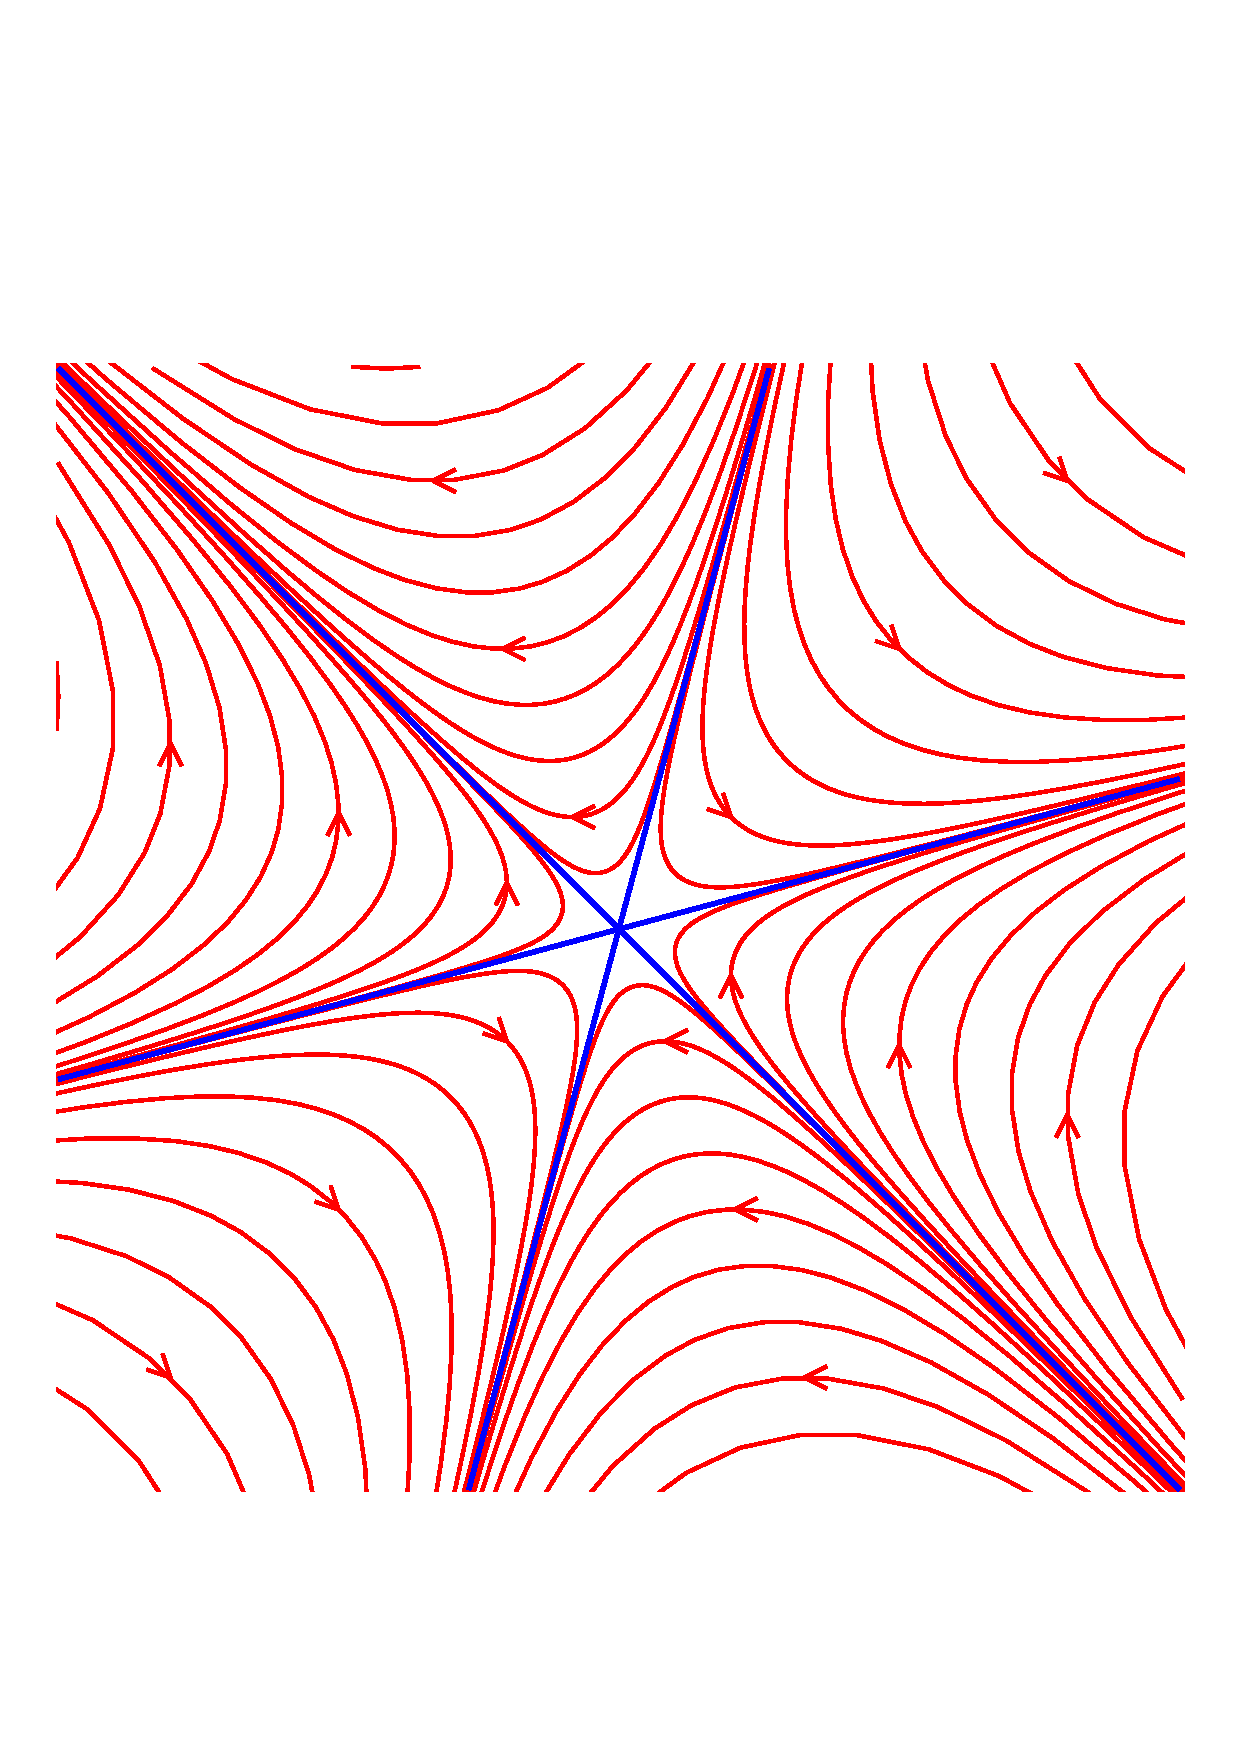
\includegraphics[scale=0.4]{../lectures/images/fluid.pdf} \]
\end{solution}

\begin{exercise}\label{ex-limit-line}
 The system 
 \begin{align*}
  \dot{x} = -x+(x^2-y^2)/4 \\
  \dot{y} = y-(x^2-y^2)/4.
 \end{align*}
 has the following phase portrait:
 \[ \includegraphics[scale=0.4]{../lectures/images/limit_line_0.pdf} \]
 \begin{itemize}
  \item[(a)] Find and classify the equilibrium points.
  \item[(b)] Add some arrows to the diagram to indicate the direction
   of flow.
  \item[(c)] There are nonzero constants $a,b,c$ such that
   $(x,y)=(at,bt+c)$ is a solution.  Find these constants.
  \item[(d)] Where does your solution to~(c) appear in the phase
   portrait?
 \end{itemize}
\end{exercise}
\begin{solution}\leavevmode
 \begin{itemize}
  \item[(a)] At an equilibrium point we must have
   $\dot{x}=-x+(x^2-y^2)/4=0$ and $\dot{y}=y-(x^2-y^2)/4=0$.  Adding
   these equations gives $y-x=0$, so $y=x$.  Substituting $y=x$ in the
   relation $-x+(x^2-y^2)/4=0$ gives $x=0$.  Thus, the only
   equilibrium point is at the origin.  The Jacobian is 
   \[ J = \left[\begin{array}{cc} \partial f/\partial x & \partial f/\partial y \\
               \partial g/\partial x & \partial g/\partial y \end{array}\right]
        = \left[\begin{array}{cc} -1+x/2 & -y/2 \\
               -x/2 & 1+y/2 \end{array}\right].
   \]
   At the origin this becomes $J=\bbm -1&0 \\ 0&1\ebm$.  As this is a
   diagonal matrix, the eigenvalues are just the diagonal entries,
   which are $1$ and $-1$.  As one eigenvalue is positive and the
   other is negative, we have a saddle.
  \item[(b)]
   \begin{itemize}
    \item At a point $(x,y)=(u,u)$ with $u>0$ we have
     $\dot{x}=-u+(u^2-u^2)/4=-u<0$ and $\dot{y}=u>0$ so the flow line
     points up and to the left. 
    \item At a point $(x,y)=(u,-u)$ with $u>0$ we have
     $\dot{x}=-u=-u<0$ and $\dot{y}=-u<0$ so the flow line points down
     and to the left.
    \item At a point $(x,y)=(-u,u)$ with $u>0$ we have
     $\dot{x}=u>0$ and $\dot{y}=u>0$ so the flow line points up
     and to the right.
    \item At a point $(x,y)=(-u,-u)$ with $u>0$ we have
     $\dot{x}=u>0$ and $\dot{y}=-u<0$ so the flow line points down
     and to the right.
   \end{itemize}
   For the actual picture, see part~(d).
  \item[(c)] If $x=at$ and $y=bt+c$ then
   \begin{align*}
    \dot{x} &= a \\
    \dot{y} &= b \\
    -x+(x^2-y^2)/4 &= -at + (a^2t^2-b^2t^2-2bct-c^2)/4 \\
      &= \tfrac{1}{4}(a^2-b^2)t^2 - (\half bc+a)t -\tfrac{1}{4}c^2 \\ 
    y-(x^2-y^2)/4 &= bt+c - (a^2t^2-b^2t^2-2bct-c^2)/4 \\
      &= \tfrac{1}{4}(b^2-a^2)t^2 + (\half bc+b)t +(c + \tfrac{1}{4}c^2). 
   \end{align*}
   Thus, we have a solution if the following equations hold for all
   $t$:
   \begin{align*}
    a &= \tfrac{1}{4}(a^2-b^2)t^2 - (\half bc+a)t -\tfrac{1}{4}c^2 \\
    b &= \tfrac{1}{4}(b^2-a^2)t^2 + (\half bc+b)t +(c - \tfrac{1}{4}c^2).
   \end{align*}
   We can equate the coefficients of $1$, $t$ and $t^2$ to get
   \begin{align*}
    a &= -\tfrac{1}{4}c^2 & \half bc+a &= 0 & a^2-b^2 &= 0 \\
    b &= c - \tfrac{1}{4}c^2 & \half bc+b &= 0 & b^2-a^2 &= 0.
   \end{align*}
   As $\half bc+a$ and $\half bc+b$ are both zero, we must have $b=a$.
   We can substitute this in $\half bc+a=0$ to get $a(c+2)=0$ but
   $a\neq 0$ by assumption, so $c=-2$.  We now have
   $a=-\tfrac{1}{4}c^2=-1$ and $b=a=-1$.  Thus,
   the relevant solution is $(x,y)=(-t,-t-2)$.  This covers the
   line where $x-y=2$.
  \item[(d)] This picture shows the direction arrows from~(a) as well
   as the solution from~(c) (in blue).
  \[ 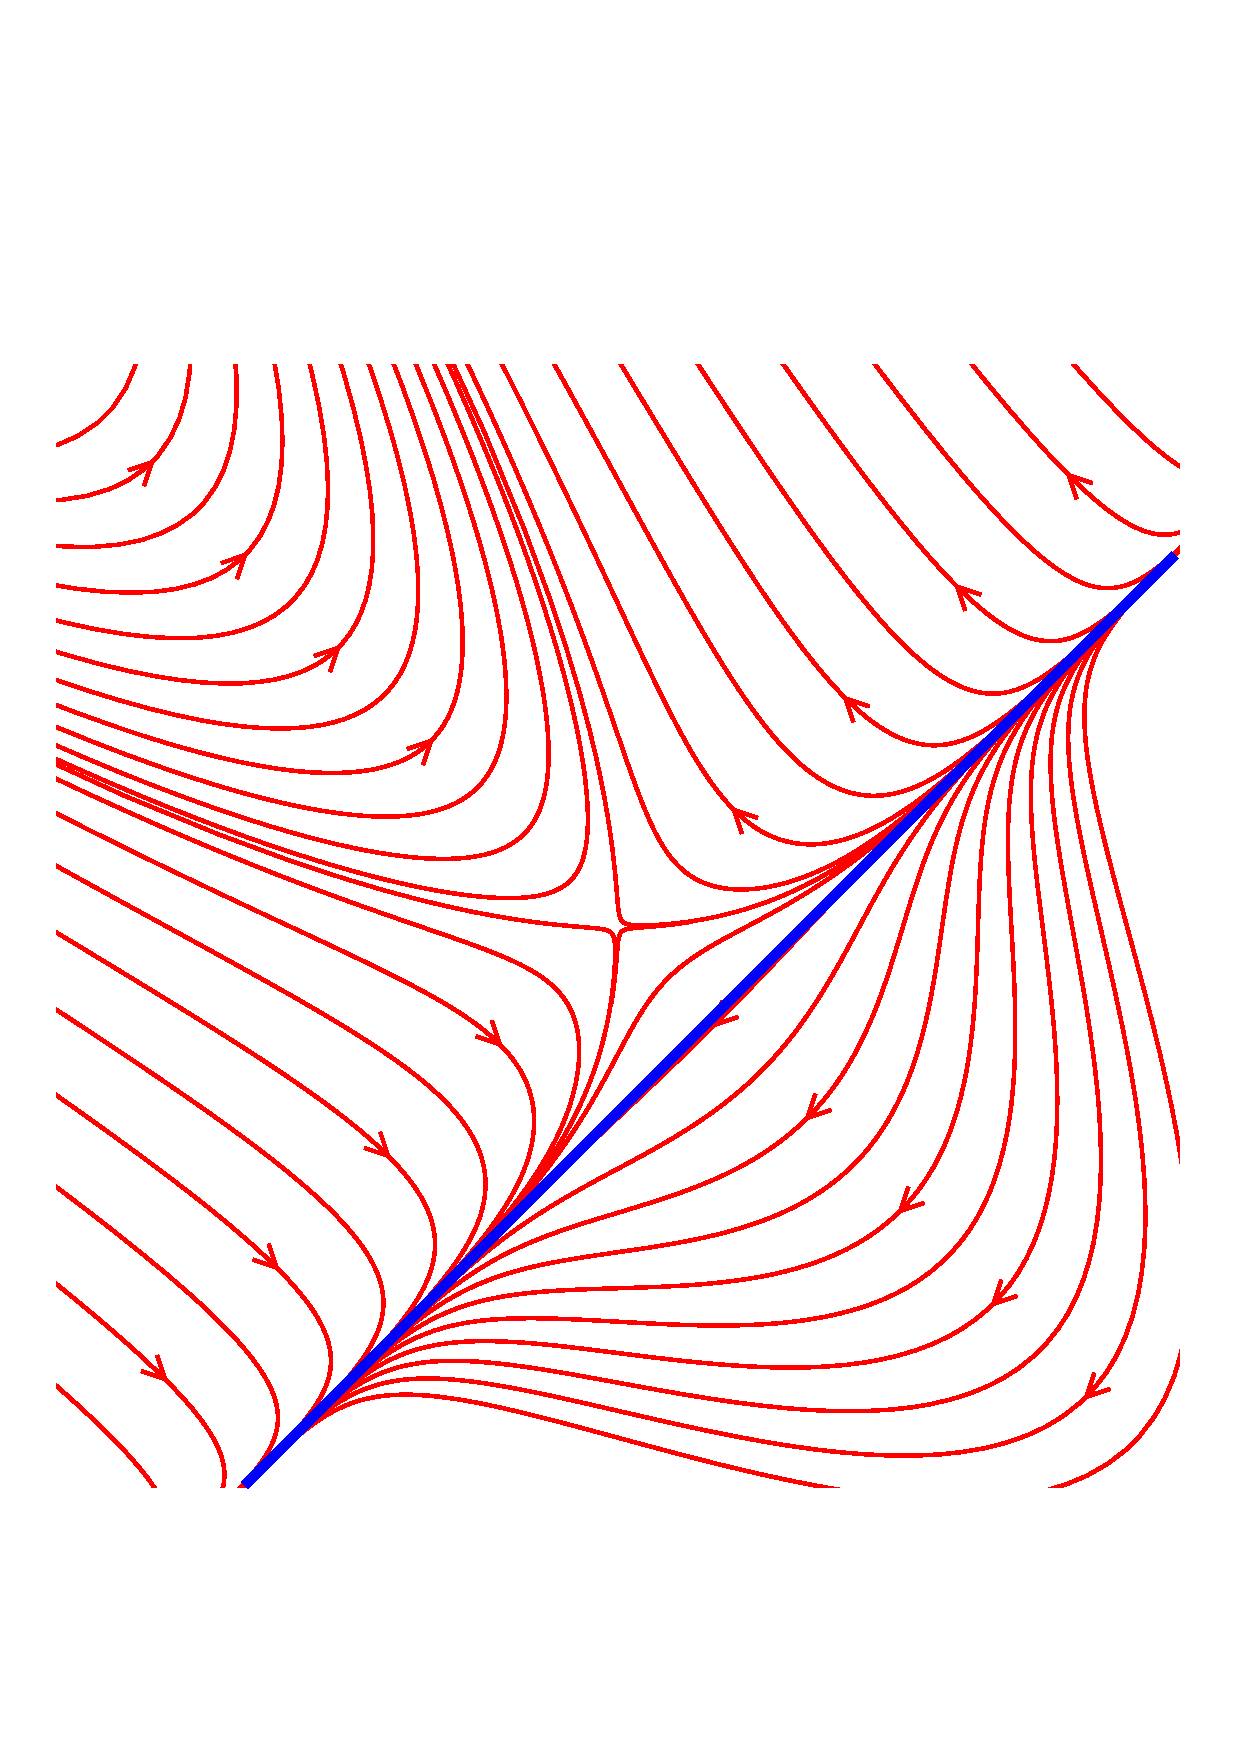
\includegraphics[scale=0.4]{../lectures/images/limit_line_1.pdf} \]
 \end{itemize}
\end{solution}

\begin{exercise}\label{ex-limit-cycle}
 Consider the system
 \begin{align*}
  \dot{x} &= f(x,y) = x-y-x^3-xy^2 \\
  \dot{y} &= g(x,y) = x+y-x^2y-y^3.
 \end{align*}
 Put $U=x^2+y^2$ and $V=1/U-1$ and $W=\arctan(y/x)$.  Show that
 $\dot{U}=2(U-U^2)$ and $\dot{V}=-2V$ and $\dot{W}=1$.  Using this,
 solve the equations, and show that there is a limit cycle.
\end{exercise}
\begin{solution}
 First, we have
 \begin{align*}
  \dot{U} &= U_xf + U_yg 
           = 2x(x-y-x^3-xy^2) + 2y(x+y-x^2y-y^3) \\
          &= 2x^2-2xy-2x^4-2x^2y^2+2xy+2y^2-2x^2y^2-2y^4 \\
          &= 2x^2+2y^2-2x^4-4x^2y^2-2y^4 = 2U-2U^2.
 \end{align*}
 This gives
 \begin{align*}
  \dot{V} &= -U^{-2}\dot{U} 
           = -2U^{-2}(U-U^2) 
           = -2(U^{-1}-1) = -2V.
 \end{align*}
 It follows that $V=V_0e^{-2t}$ for some constant $V_0$, and so
 $U=1/(1+V)=1/(1+V_0e^{-2t})$.  

 Next, remember that $\arctan'(t)=1/(1+t^2)$.  This gives
 \begin{align*}
  \dot{W} &= \frac{d(y/x)/dt}{1+(y/x)^2} 
           = \frac{(\dot{y}x-y\,\dot{x})/x^2}{1+(y/x)^2} 
           = \frac{gx-yf}{x^2+y^2} \\
  gx-yf   &= (x+y-x^2y-y^3)x - y(x-y-x^3-xy^2) \\
          &= x^2+xy-x^3y-xy^3 - xy + y^2+x^3y+xy^3 
           = x^2+y^2 \\
  \dot{W} &= 1.
 \end{align*}
 This means that $W=W_0+t$ for some constant $t$.  Now, the polar
 coordinates of $(x,y)$ are $r=\sqrt{U}=(1+V_0e^{-2t})^{-1/2}$ and
 $\tht=W=W_0+t$, so we have
 \begin{align*}
  x &= (1+V_0e^{-2t})^{-1/2}\cos(W_0+t) \\
  y &= (1+V_0e^{-2t})^{-1/2}\sin(W_0+t).
 \end{align*}
 As $t\to\infty$ we have $e^{-2t}\to 0$ and so $U\to 1$, which means
 that 
 \[ \bbm x\\ y\ebm \simeq \bbm \cos(W_0+t) \\ \sin(W_0+t) \ebm, \]
 so the solution curve approaches the unit circle, which is a limit
 cycle for the system.
\end{solution}

\begin{exercise}\label{ex-misc-c}
 Find and classify the equilibrium points for the system
 \begin{align*}
  \dot{x} &= f(x,y) = x^2+2y^2-y \\
  \dot{y} &= g(x,y) = 2x+2y.
 \end{align*}
\end{exercise}
\begin{solution}
 For an equilibrium point we must have $x^2+2y^2-y=0$ and $2x+2y=0$.
 The second equation gives $y=-x$, and substituting this into the
 first equation gives $3x^2+x=0$ or $x(3x+1)=0$.  We thus have $x=0$
 or $x=-1/3$, so the two equilibria are $a_1=(0,0)$ and
 $a_2=(-1/3,1/3)$.  The Jacobian is 
 \[ J = \left[\begin{array}{cc} \partial f/\partial x & \partial f/\partial y \\
             \partial g/\partial x & \partial g/\partial y \end{array}\right]
      = \left[\begin{array}{cc} 2x & 4y-1 \\ 2 & 2 \end{array}\right].
 \]
 Evaluating this at the equilibrium points gives
 \[ J_1 = \left[\begin{array}{cc} 0 & -1 \\ 2 & 2 \end{array}\right] \hspace{4em}
    J_2 = \left[\begin{array}{cc} -2/3 & 1/3 \\ 2 & 2 \end{array}\right].
 \]
 For $J_1$ we have $\tau=2$ and $\delta=2$ so $\tau^2-4\delta=-4<0$.  As
 $\tau>0$ and $\tau^2-4\delta<0$ we see that the point $a_1$ is an
 unstable focus.  As the bottom left entry in $J$ is positive, it is an
 anticlockwise focus.  

 For $J_2$ we have $\tau=4/3$ and $\delta=-2$.  As $\delta<0$, this is a
 saddle.    

 \[ \includegraphics[scale=0.4]{../lectures/images/misc_c.pdf} \]
\end{solution}

\begin{exercise}\label{ex-competition}
 Analyse the following system (which describes the populations of two
 species that compete for food):
 \[ \dot{x} = 2x(1-x-y) \hspace{4em} \dot{y} = y(1-2y-2x). \]
\end{exercise}
\begin{solution}
 On the $x$-nullcline we have $2x(1-x-y)=0$, so either $x=0$ or
 $y=1-x$.  On the $y$-nullcline we have $y(1-2y-2x)=0$, so either
 $y=0$ or $y=\half-x$.  In principle there are now four possibilities
 for $(x,y)$, but the equations $y=1-x$ and $y=\half-x$ are
 incompatible, so in fact there are only three:
 \begin{itemize}
  \item The origin is an equilibrium point $a_1=(0,0)$.
  \item There is another equilibrium point with $x=0$ and $y=\half-x$, so
   $y=\half$, so the point is $a_2=(0,\half)$.
  \item There is another equilibrium point with $y=1-x$ and $y=0$,
   so $x=1$, so the point is $a_3=(1,0)$.
 \end{itemize}
 Recall that 
 \begin{align*}
  f &= 2x(1-x-y) = 2x - 2x^2 - 2xy \\
  g &= y(1-2y-2x) = y - 2y^2 - 2xy.
 \end{align*}
 The Jacobian is 
 \[ J = \left[\begin{array}{cc} \partial f/\partial x & \partial f/\partial y \\
             \partial g/\partial x & \partial g/\partial y \end{array}\right]
      = \left[\begin{array}{cc} 2-4x-2y & -2x \\ -2y & 1-4y-2x \end{array}\right].
 \]
 Evaluating this at the equilibrium points gives
 \begin{align*}
  J_1 &= \bbm 2 & 0 \\ 0 & 1 \ebm \\
  J_2 &= \bbm 1 & 0 \\ -1 & -1 \ebm \\
  J_3 &= \bbm -2 & -2 \\ 0 & -1 \ebm.
 \end{align*}
 Recall that for a matrix of the form $\bbm a&0\\ c&d\ebm$ or
 $\bbm a&b\\ 0&d\ebm$, the eigenvalues are just the same as the
 diagonal entries $a$ and $d$.  Thus, the eigenvalues for $J_1$ are
 $1$ and $2$ (so $a_1$ is an unstable node), the eigenvalues for $J_2$
 are $1$ and $-1$ (so $a_2$ is a saddle), and the eigenvalues for $J_3$
 are $-2$ and $-1$ (so $a_3$ is a stable node).

 The phase portrait is as follows:
 \[ 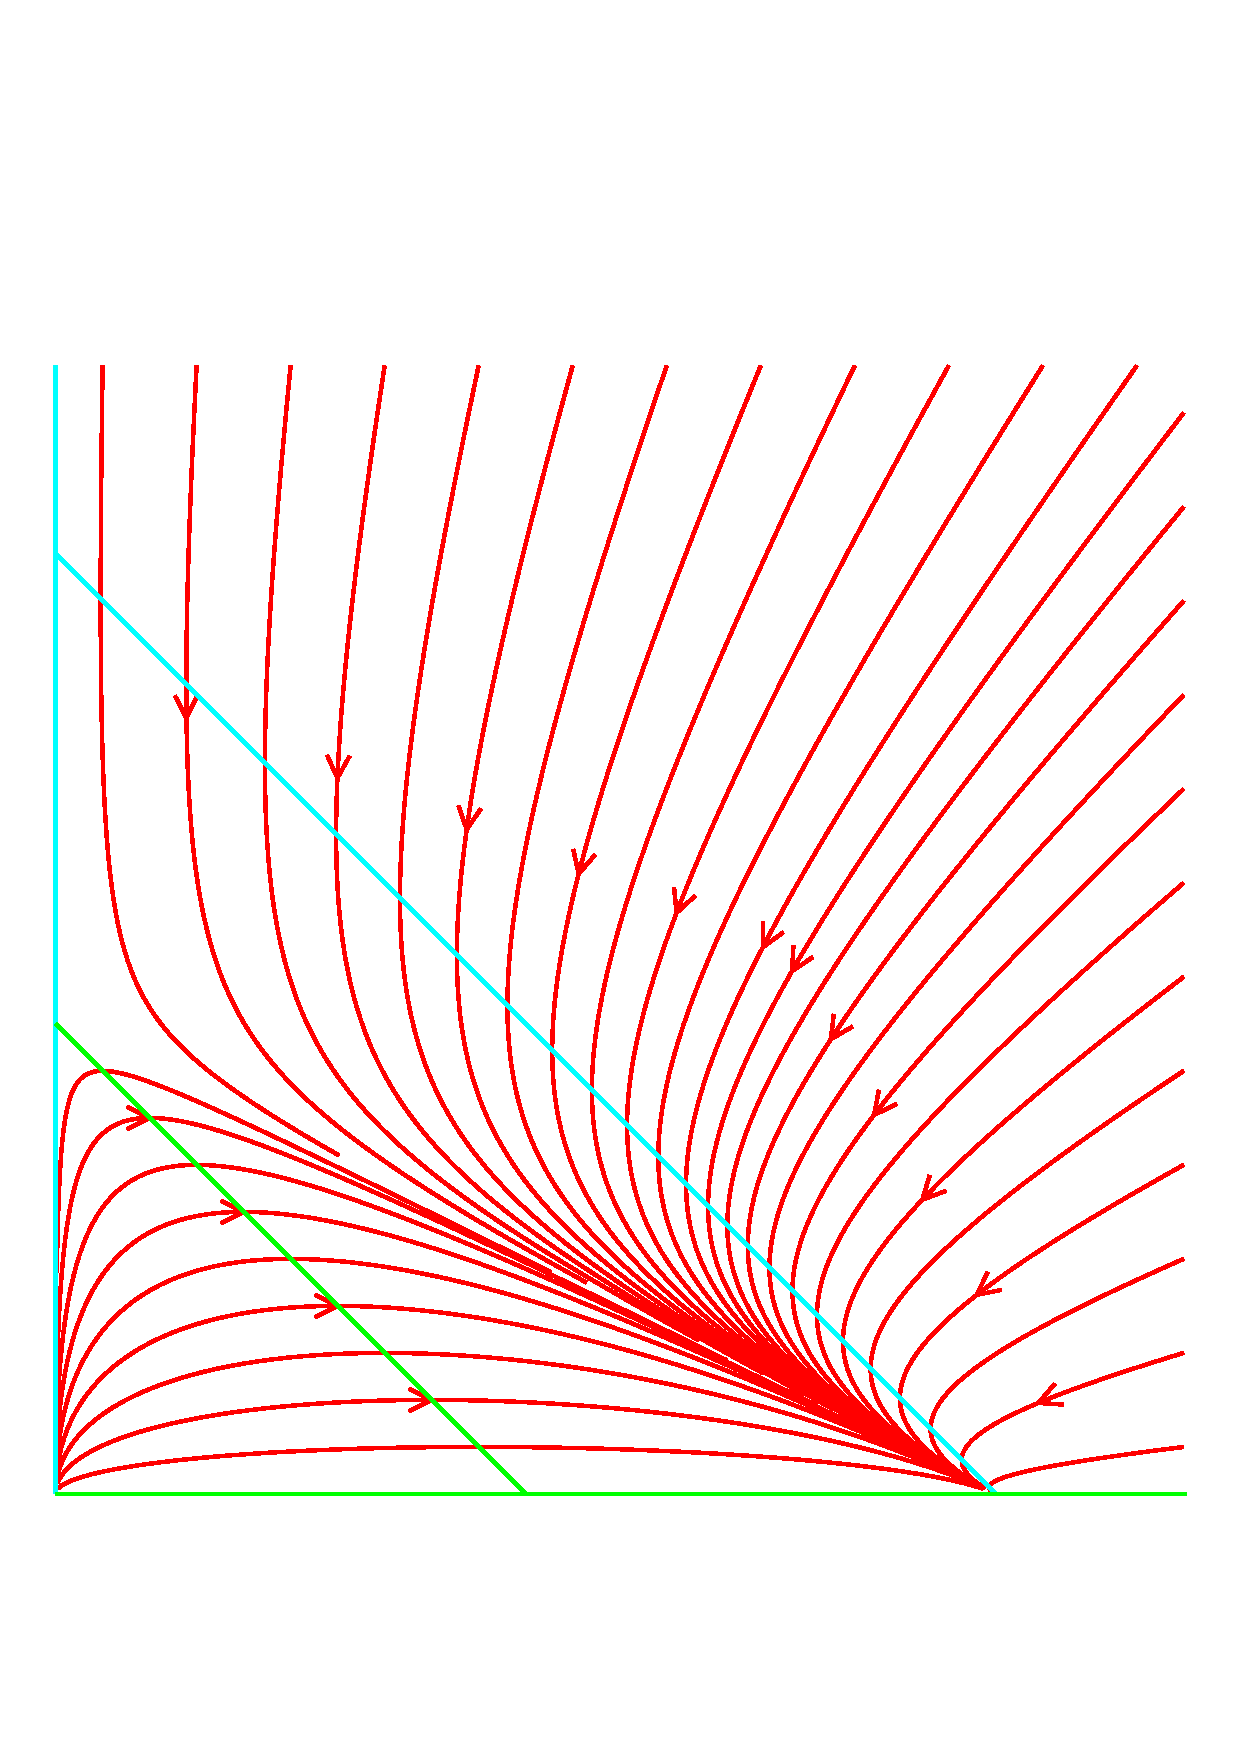
\includegraphics[scale=0.2]{../lectures/images/competition.pdf} \]
 The variables $x$ and $y$ represent populations of competing species,
 so they cannot be negative, so we have shown only the region where
 $x\geq 0$ and $y\geq 0$.  All the flow lines converge to $a_3$, where
 $x=1$ and $y=0$.  This means that the $y$ species will become extinct
 and will be replaced by the $x$ species.
\end{solution}

\begin{exercise}\label{ex-parallel}
 Consider a system of the form $\dot{x}=\dot{y}=f(x,y)$.  What can you
 say about the phase portrait?
\end{exercise}
\begin{solution}
 As $\dot{y}=\dot{x}$, the difference $y-x$ is constant, so each flow
 line is (part of) a straight line $y=x+c$.  This means that the exact
 form of the function $f$ is mostly irrelevant, the phase portrait
 just looks like this:
 \[ \includegraphics[scale=0.2]{../lectures/images/parallel.pdf} \]
\end{solution}

\begin{exercise}\label{ex-y-shift}
 Consider a system of the form $\dot{x}=1$, $\dot{y}=f'(x)$, for some
 given function $f$ with $f(0)=0$.  What can you say about the
 solutions and the phase portrait? 
\end{exercise}
\begin{solution}
 Consider a solution that starts at a point $(0,y_0)$ on the
 $y$-axis.  We have $\dot{x}=1$ so $x=t+c$ for some constant $c$, but
 $x=0$ when $t=0$, so $x=t$.  We also have $\dot{y}=f'(x)=f'(t)$, so
 $y-f(t)$ is constant, say $y=f(t)+d$.  At $t=0$ we have $y=y_0$ and
 $f(0)=0$ so $d=y_0$.  This means that the solution is just
 $y=f(t)+y_0$.  In particular, all the solutions are the same except
 for the vertical shift by $y_0$.  Thus, the phase portrait might look
 something like this:
 \[ 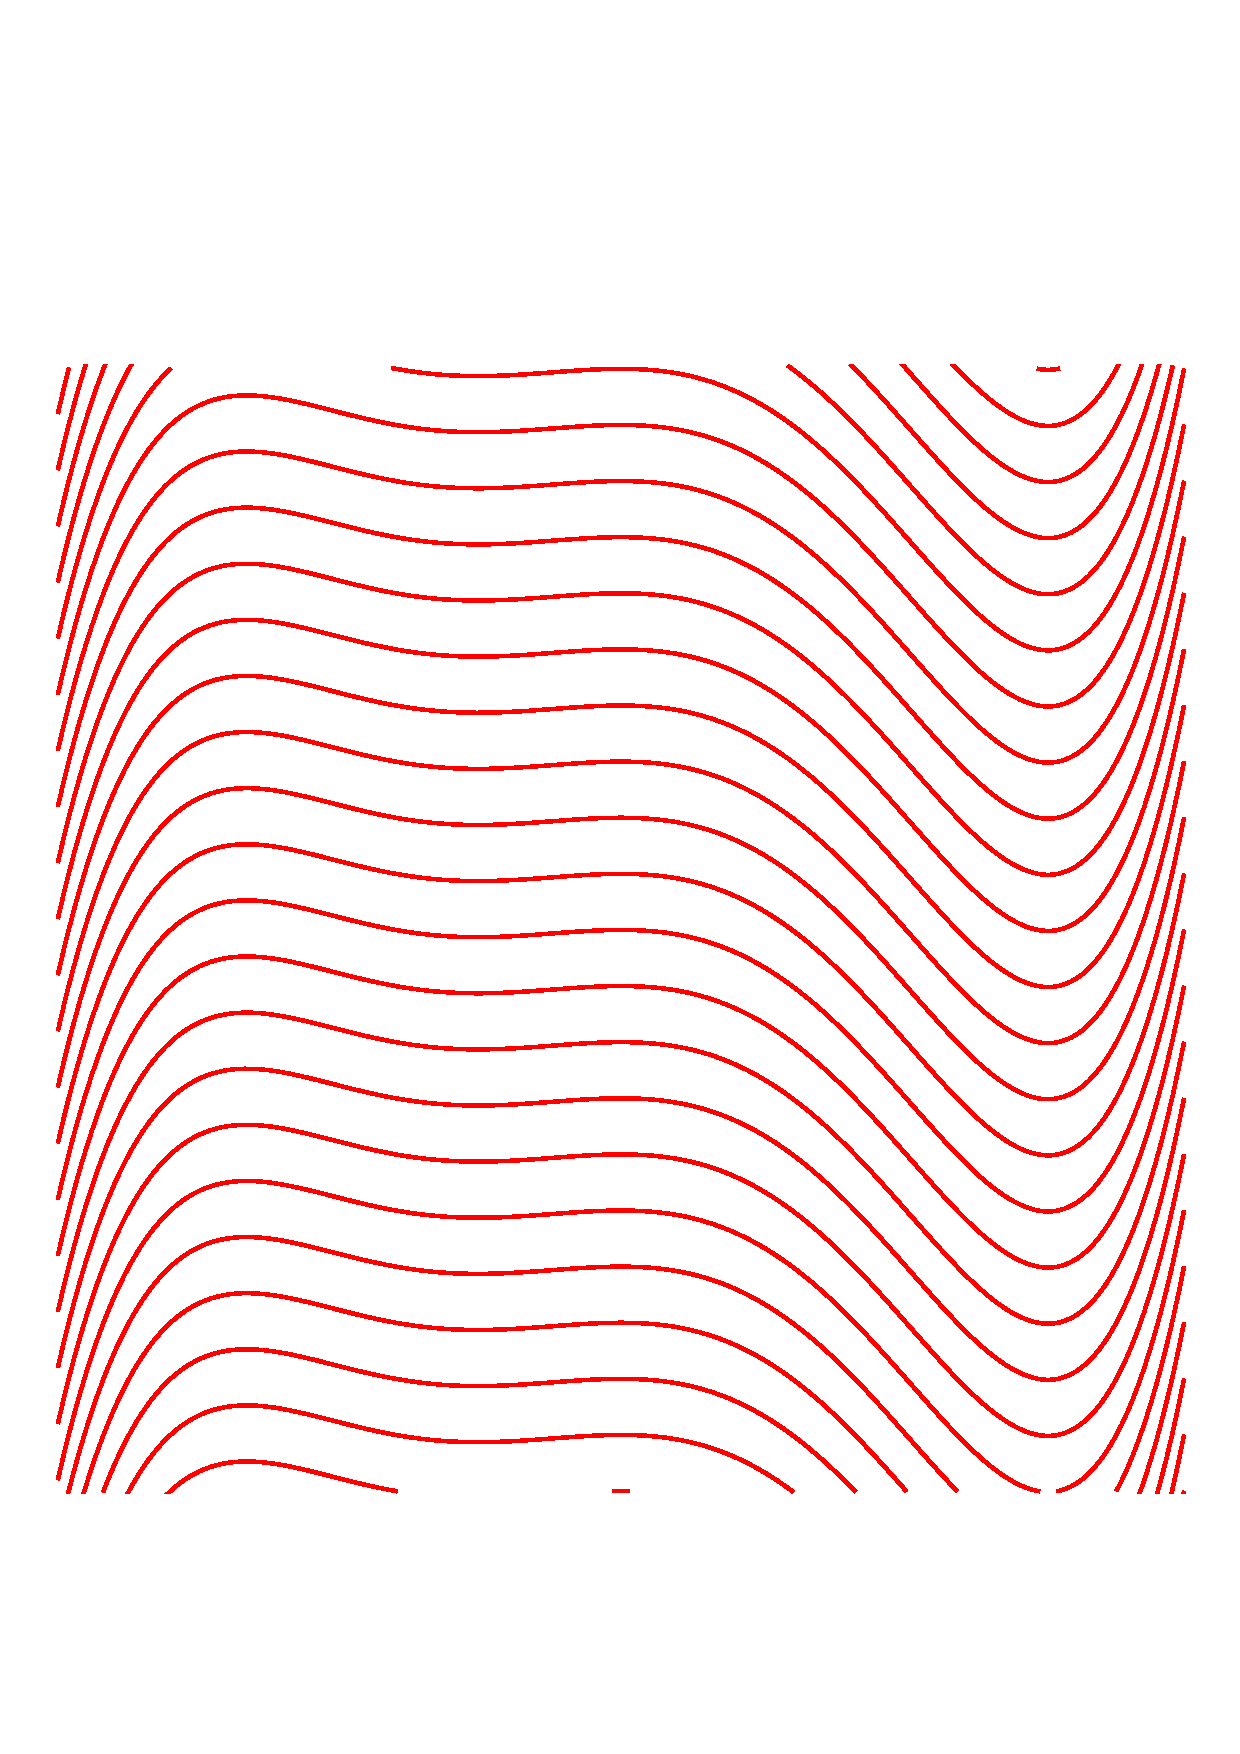
\includegraphics[scale=0.2]{../lectures/images/y_shift.pdf} \]
\end{solution} 

\begin{exercise}\label{ex-quad-definite}
 For each of the following quadratic functions, decide whether it is
 positive definite, negative definite or indefinite.
 \begin{align*}
  Q_1 &= xy & Q_2 &= x^2-y^2 & Q_3 &= (x+y)^2 \\
  Q_4 &= x^2+xy+y^2 & Q_5 &= 3x^2-4xy+5y^2 & Q_6 &=8xy-3x^2-5y^2.
 \end{align*}
\end{exercise}
\begin{solution}\leavevmode
 \begin{itemize}
  \item $Q_1$ is indefinite because $Q_1=0$ at $(x,y)=(0,1)$.
  \item $Q_2$ is indefinite because $Q_2=0$ at $(x,y)=(1,1)$.
  \item $Q_3$ is indefinite because $Q_3=0$ at $(x,y)=(1,-1)$.
  \item $Q_4$ is positive definite.  To see this, note that
   $Q_4=ax^2+2bxy+cy^2$ with $a=c=1$ and $b=\half$.  Here
   $ac-b^2=\frac{3}{4}>0$ and $a,c>0$, so the standard method tells us
   that $Q_4$ is positive definite.  Alternatively, one can check that 
   \[ Q_4 = \frac{3}{4}(x+y)^2 + \frac{1}{4}(x-y)^2. \]
   From this it is clear that $Q_4\geq 0$, and that $Q_4$ can only be
   equal to $0$ if $x+y=0$ and $x-y=0$, which means that $x=y=0$.
  \item $Q_5$ is again positive definite.  Indeed, here we have $a=3$
   and $b=-2$ and $c=5$ so $a,c>0$ and $ac-b^2=11>0$.
  \item $Q_6$ is indefinite.  Indeed, here we have $a=-3$ and $b=4$
   and $c=-5$ so $ac-b^2=-1<0$.  Alternatively, we can just note that
   $Q_6=0$ when $(x,y)=(1,1)$.
 \end{itemize}
\end{solution}

\begin{exercise}\label{ex-definite}
 For each of the following functions, discuss whether it is positive
 definite, negative definite or indefinite about the origin, either on
 the whole plane or on some smaller domain.
 \begin{align*}
  V_1 &= e^{-x^2-y^2} & V_2 &= e^{-x^2-y^2}-1 & V_3 &= 2-\cos(x)-\cos(y) \\
  V_4 &= x^3+x^2y+xy^2+y^3 & V_5 &= \frac{x^2+y^2}{1+x^2+y^2} & V_6 &= \frac{x^2+y^2}{1-x^2-y^2}
 \end{align*}
\end{exercise}
\begin{solution}\leavevmode
 \begin{itemize}
  \item As $e^t>0$ for all $t$, we have $V_1>0$ at all points
   $(x,y)$.  In particular, $V_1=1$ at $(0,0)$, but we only say that a
   function is positive definite around the origin if it takes the
   value $0$ at the origin.  Thus, $V_1$ is not positive definite.
  \item At $(x,y)=(0,0)$ we have $x^2+y^2=0$ so $V_2=e^0-1=0$.  At all
   other points, we have $x^2+y^2>0$ so $e^{-x^2-y^2}<1$ so $V_2<0$.
   Thus, $V_2$ is negative definite.
  \item For all $x$ and $y$ we have $-1\leq\cos(x),\cos(y)\leq 1$ and
   so $V_3=(1-\cos(x))+(1-\cos(y))\geq 0$.  From this it is also clear
   that $V_3$ can only be zero if $\cos(x)=1$ and $\cos(y)=1$, which
   means that $x$ and $y$ are both multiples of $2\pi$.  In
   particular, $V_3$ is zero at the point $(2\pi,0)$, which means that
   $V_3$ is not positive definite on the whole plane.  However, we can
   instead put 
   \[ R = \{(x,y)\st -2\pi < x,y < 2\pi\}. \]
   We find that the only point in $R$ where $V_3=0$ is $(0,0)$, so
   $V_3$ is positive definite about the origin on $R$.
  \item The function $V_4$ is zero at $(x,y)=(1,-1)$, so $V_4$ is
   neither positive definite nor negative definite on the whole
   plane.  In fact, for any small $\ep>0$ we have a point $(\ep,-\ep)$
   (very close to the origin) where $V_4=0$.  This means that $V_4$ is
   not positive or negative definite on any neighbourhood of the
   origin.
  \item As $x^2+y^2\geq 0$ and $1+x^2+y^2>0$ for all $x,y$ we find
   that $V_5\geq 0$ everywhere.  Moreover, $V_5$ can only be zero if
   $x^2+y^2=0$ which means that $x=y=0$.  Thus, $V_5$ is positive
   definite on the whole plane.
  \item The function $V_6$ is undefined if $x^2+y^2=1$, and is
   negative if $x^2+y^2>1$.  Thus, we should consider only the domain 
   \[ R = \{(x,y)\st x^2+y^2<1\}, \]
   which is an open disc centred at the origin.  In this region we
   have $x^2+y^2\geq 0$ and $1-x^2-y^2>0$ so $V_6\geq 0$.  Moreover,
   $V_6$ can only be zero if $x^2+y^2=0$ which means that $x=y=0$.
   Thus, $V_6$ is positive definite on the region $R$.
 \end{itemize}
\end{solution}

\begin{exercise}\label{ex-odd-indefinite}
 Consider a function of the form $V=ax^5+bx^4y+cxy^4+dy^5$, where $a$,
 $b$, $c$ and $d$ are constants.  Show that $V$ is neither positive
 definite nor negative definite around the origin.
\end{exercise}
\begin{solution}
 At $(1,0)$ we have $V=a$, and at $(-1,0)$ we have $V=-a$.  These
 cannot both be strictly positive, so $V$ is not positive definite.
 Similarly, $a$ and $-a$ cannot both be strictly negative, so $V$ is
 not negative definite.
\end{solution}

\begin{exercise}\label{ex-conserved-constant}
 Suppose we have a linear system $\dot{u}=Au$ with a stable node or a
 stable focus at the origin, and that $U$ is a conserved quantity that
 is defined and continuous over the whole plane.  Show that $U$ is
 just a constant.
\end{exercise}
\begin{solution}
 Put $C=U(0,0)$ (the value of the conserved quantity at the origin).
 Consider an arbitrary point $(x_0,y_0)$.  Let $(x,y)$ be the solution
 that starts at $(x_0,y_0)$ at time $t=0$.  As the system is a stable
 node or focus, we have $(x,y)\to(0,0)$ as $t\to\infty$.  As $U$ is
 continuous, we have $U(x,y)\to U(0,0)=C$ as $t\to\infty$.  However,
 $U$ is a conserved quantity, so $U(x,y)$ is independent of $t$.  The
 only way it can be independent of  $t$ and converge to $C$ is if it
 is equal to $C$ all the time.  We thus have $U(x,y)=C$ for all $t$,
 so in particular this holds when $t=0$, which means that
 $U(x_0,y_0)=C$.  This holds for all $x_0$ and $y_0$, so $U$ is
 constant. 
\end{solution}

\begin{exercise}\label{ex-lyapunov-a}
 Consider the system 
 \[ \dot{x} = -2y^3 \hspace{4em} \dot{y} = x-3y^3. \]
 Find a Lyapunov function $V$ of the form $V=ax^2+by^4$ (for some
 constants $a$ and $b$).  Deduce that the origin is a stable
 equilibrium point.
\end{exercise}
\begin{solution}
 Consider a function $V=ax^2+by^4$.  We want $V$ to be positive
 definite, so we must have $a,b>0$.  Note that 
 \[ \dot{V} = V_x\dot{x} + V_y\dot{y} = 
     2ax(-2y^3) +4by^3(x-3y^3) = 
      (4b-4a)xy^3 - 12by^6.
 \]
 The term $xy^3$ can be positive or negative depending on the signs of
 $x$ and $y$.  It is simplest to make this term go away by choosing
 $a=b=1$.  Out function is then $V=x^2+y^4$, with $\dot{V}=-12y^6$.
 This means we always have $\dot{V}\leq 0$, but $\dot{V}=0$ everywhere
 on the $x$-axis, so $\dot{V}$ is negative semidefinite but not
 negative definite.  Thus, $V$ is a weak Lyapunov function but not a
 strong Lyapunov function, and the origin is stable but not
 necessarily asymptotically stable.  (In fact the origin \emph{is}
 asymptotically stable, but we need a different argument to prove it.)
\end{solution}

\begin{exercise}\label{ex-lyapunov-b}
 Consider the system 
 \[ \dot{x} = -3x^3 - y \hspace{4em} \dot{y} = x^5 - 2y^3. \]
 Find a Lyapunov function of the form $V=\al x^{2n}+\bt y^{2m}$ (for
 certain constants $\al,\bt,n,m$), and deduce that the origin is a
 stable equilibrium point.  Can we conclude that it is asymptotically
 stable? 
\end{exercise}
\begin{solution}
 Consider a function $V=\al x^{2n}+\bt y^{2m}$.  If we take $n$ and
 $m$ to be positive integers and $\al,\bt>0$ then $V$ will be positive
 definite.  We also have
 \begin{align*}
  \dot{V} &= V_x\dot{x} + V_y\dot{y} 
           = 2n\al x^{2n-1}(-3x^3-y) + 2m\bt y^{2m-1}(x^5-2y^3) \\
          &= -6n\al x^{2n+2} 
             -2n\al x^{2n-1}y 
             +2m\bt x^5y^{2m-1}
             -4m\bt y^{2m+2}.
 \end{align*}
 The middle two terms have odd exponents, so they can be either
 positive or negative.  It is best to make them cancel out.  For that,
 we need $2n\al=2m\bt$ and $2n-1=5$ and $2m-1=1$.  This gives $m=1$
 and $n=3$ and $6\al=2\bt$.  We can choose $\al=1$ and then $\bt=3$.
 With these choices, the function becomes $V=x^6+3y^2$, and
 \[ \dot{V} = -6n\al x^{2n+2} - 4m\bt y^{2m+2} = -18x^8-12y^4. \]
 It is clear from this that $\dot{V}$ is negative definite, so $V$ is
 a strong Lyapunov function, and the origin is an asymptotically
 stable equilibrium.
\end{solution}

\begin{exercise}\label{ex-lyapunov-c}
 Consider the system 
 \[ \dot{x} = y \hspace{4em} \dot{y} = -x + y(x^2+y^2-1). \]
 Find a Lyapunov function of the form $V=\al x^{2n}+\bt y^{2m}$ (for
 certain constants $\al,\bt,n,m$), and deduce that the origin is a
 stable equilibrium point.  Can we conclude that it is asymptotically
 stable? 
\end{exercise}
\begin{solution}
 Consider a function $V=\al x^{2n}+\bt y^{2m}$.  If we take $n$ and
 $m$ to be positive integers and $\al,\bt>0$ then $V$ will be positive
 definite.  We also have
 \begin{align*}
  \dot{V} &= V_x\dot{x} + V_y\dot{y} 
           = 2n\al x^{2n-1}y + 
             2m\bt y^{2m-1}(-x + y(x^2+y^2-1)) \\
   &= 2n\al x^{2n-1}y - 2m\bt xy^{2m-1} - 2m\bt y^{2m}(1-x^2-y^2).
 \end{align*} 
 The first two terms have odd exponents, so they can be either
 positive or negative.  It is best to make them cancel out.  For that,
 we need $2n-1=1$ and $2m-1=1$ and $2n\al=2m\bt$, so $n=m=1$ and
 $\al=\bt$.  We choose $\al=1$, so $V=x^2+y^2$ and 
 \[ \dot{V} = -2m\bt y^2(1-x^2-y^2) = -2y^2(1-x^2-y^2). \]
 If we restrict attention to the unit disc
 \[ R = \{(x,y)\st x^2+y^2 < 1\}, \]
 then we have $\dot{V}\leq 0$.  This means that $V$ is a weak Lyapunov
 function, so the origin is a stable equilibrium point.  However, we
 have $\dot{V}=0$ at all points where $y=0$, so $V$ is not a strong
 Lyapunov function, and we cannot immediately conclude that the origin
 is asymptotically stable.
\end{solution}

\begin{exercise}\label{ex-lyapunov-linear}
 Consider a linear system $\dot{x}=py-qx$,\; $\dot{y}=rx-sy$ where
 $p,q,r,s>0$ and $4qs>(p+r)^2$.
 \begin{itemize}
  \item[(a)] Show that the function $x^2+y^2$ is a strong Lyapunov
   function.
  \item[(b)] Show that $qs-pr>0$.
  \item[(c)] Classify the equilibrium point at the origin.
 \end{itemize}
\end{exercise}
\begin{solution}\leavevmode
 \begin{itemize}
  \item[(a)] It is clear that $V$ is positive definite.  First, we have 
   \[ \dot{V} = 2x\dot{x} + 2y\dot{y} = 
       2pxy - 2qx^2 + 2rxy -2sy^2 = 
       -2qx^2 + 2(p+r)xy - 2sy^2.
   \]
   In other words, we have $\dot{V}=ax^2+2bxy+cy^2$, where $a=-2q$ and
   $b=p+r$ and $c=-2s$.  The standard criterion says that $\dot{V}$ is
   negative definite if $a,c<0$ and $ac>b^2$, or equivalently $q,s>0$
   and $4qs>(p+r)^2$.  These are precisely the assumptions in the
   question, so $\dot{V}$ is negative definite.  This means that $V$
   is a strong Lyapunov function, and that the origin is an
   asymptotically stable equilibrium point.
  \item[(b)] We are given that $4qs>(p+r)^2$, so 
   \[ 4qs - 4pr > (p+r)^2 - 4pr = p^2 + 2pr + r^2 - 4pr =
       p^2 - 2pr + r^2 = (p-r)^2 \geq 0.
   \]
   This shows that $4qs-4pr>0$, so $qs-pr>0$.
  \item[(c)] The system can be written as
   $\bbm\dot{x}\\ \dot{y}\ebm = A \bbm x \\ y \ebm$, where 
   $A=\bbm -q&p \\ r&-s\ebm$.  This has trace $\tau=-(q+s)<0$ and
   determinant $\dl=qs-pr>0$ (by part~(b)).  We also have 
   \begin{align*}
    \tau^2-4\dl &= (q+s)^2 - 4qs + 4pr = q^2 + 2qs + s^2 - 4qs + 4pr\\
     &= q^2 - 2qs + s^2 + 4pr = (q-s)^2 + 4pr.
   \end{align*}
   Now $p,r>0$ by assumption, so $4pr>0$, and $(q-s)^2\geq 0$
   automatically, so $\tau^2-4\dl>0$.  As $\dl>0$ and $\tau<0$ and
   $\tau^2-4\dl>0$, we have a stable node at the origin.
   \begin{center}
    \begin{tikzpicture}[scale=2.5]
     \fill[gray!20] (-1,0) -- (0,0) -- (0,1) -- (-1,1) -- cycle;
     \draw[thick,cyan] (-1,0) -- (0,0);
     \draw[thick,orange,->] (0,0) -- (1,0);
     \draw[thick,olivegreen,->] (0,0) -- (0,1);
     \draw[thick,blue,smooth] (-1,1) -- (-0.9,0.81) -- (-0.8,0.64) --
       (-0.7,0.49) -- (-0.6,0.36) -- (-0.5,0.25) -- (-0.4,0.16) --
       (-0.3,0.09) -- (-0.2,0.04) -- (-0.1,0.01) -- (0,0);
     \draw[thick,red,smooth] (1,1) -- (0.9,0.81) -- (0.8,0.64) --
       (0.7,0.49) -- (0.6,0.36) -- (0.5,0.25) -- (0.4,0.16) --
       (0.3,0.09) -- (0.2,0.04) -- (0.1,0.01) -- (0,0);
     \draw(0,1) node[anchor=south]{$\ss\dl$};
     \draw(1,0) node[anchor=west]{$\ss\tau$};
     \draw(-0.7,0.1) node{$\ss \text{stable node}$};
    \end{tikzpicture}
   \end{center}
 \end{itemize}
\end{solution}

\begin{exercise}\label{ex-lyapunov-binomial}
 Let $\al,\bt,\gm,\dl$ be positive constants, and let $m,n,p,q$ be
 nonnegative integers.  Put 
 \begin{align*}
  f(x,y) &= -\al x^{2p+1} - (m+1)\bt y^{2m+1} \\
  g(x,y) &= (n+1)\gm x^{2n+1} - \dl y^{2q+1} \\
  V(x,y) &= \gm x^{2n+2} + \bt y^{2m+2}.
 \end{align*}
 Show that if $\dot{x}=f$ and $\dot{y}=g$ then  
 \[ \dot{V} = 
     -2(n+1)\al\gm x^{2(n+p+1)}
     -2(m+1)\bt\dl y^{2(m+q+1)},
 \]
 and so $V$ is a strong Lyapunov function for this system.
\end{exercise}
\begin{solution}
 \textbf{Write this.}
\end{solution}

\begin{exercise}\label{ex-lyapunov-e}
 Find a Lyapunov function of the form $ax^2+by^2$ for the system
 $\dot{x}=xy^2-x^3$, $\dot{y}=-(2x^2y+y^3)$.  What can we conclude
 about the nature of the equilibrium at the origin?
\end{exercise}
\begin{solution}
 If $V=ax^2+by^2$ then
 \[ \dot{V} = 2ax(xy^2-x^3) + 2by(-2x^2y-y^3)
            = 2ax^2y^2 - 2ax^4 - 4bx^2y^2 - 2by^4 
            = -2ax^4 + (2a-4b)x^2y^2 - 2by^4.
 \]
 The simplest thing to do is to choose $a=2$ and $b=1$, so
 $V=2x^2+y^2$, which is positive definite.  The equation above then
 becomes $\dot{V}=-4x^4-2y^4$, which is negative definite.  This means
 that $V$ is a strong Lyapunov function, and the origin is
 asymptotically stable.
\end{solution}

\begin{exercise}\label{ex-lyapunov-f}
 Find a Lyapunov function of the form $ax^2+by^2$ for the system
 $\dot{x}=-\half x^3+2xy^2$, $\dot{y}=-y^3$.  What can we conclude
 about the nature of the equilibrium at the origin?
\end{exercise}
\begin{solution}
 It will work out that $ax^2+by^2$ is a strong Lyapunov function
 provided that $a,b>0$ and $b>2a$.  To be definite, we will take $a=1$
 and $b=3$, so $V=x^2+3y^2$.  This is clearly positive definite.  We
 also have 
 \[ \dot{V} = 2x(-\half x^3+2xy^2) +6y(-y^3)
            = -x^4 +4x^2y^2-6y^4
            = -(x^2-2y^2)^2 -2y^4.
 \]
 From this representation it is clear that $\dot{V}\leq 0$, and that
 $\dot{V}$ can only equal zero if $x^2-2y^2=0$ and $y=0$, which gives
 $(x,y)=(0,0)$.  Thus, $\dot{V}$ is negative definite, so $V$ is a
 strong Lyapunov function, so the origin is asymptotically stable.
\end{solution}

\begin{exercise}\label{ex-lyapunov-g}
 Use quadratic Lyapunov functions to determine the stability of the
 origin for the following systems:
 \begin{itemize}
  \item[(a)] $\dot{x}=-x-2y^2$,\; $\dot{y}=xy-y^3$.
  \item[(b)] $\dot{x}=2y^2-x^3$,\; $\dot{y}=-4xy$.
 \end{itemize}
\end{exercise}
\begin{solution}\leavevmode
 \begin{itemize}
  \item[(a)] Consider the function $V=x^2+2y^2$, which is positive
   definite.  We then have 
   \[ \dot{V} = 2x(-x-2y^2) + 2y(xy-y^3) 
              = -2x^2 -4xy^2 + 4xy^2 - 2y^4 
              = -2(x^2+y^4), 
   \]
   which is negative definite.  This means that $V$ is a strong
   Lyapunov function, so the origin is asymptotically stable.
  \item[(b)] Consider the function $V=2x^2+y^2$, which is positive
   definite.  We then have 
   \[ \dot{V} = 4x(2y^2-x^3) +2y(-4xy) 
              = 8xy^2 - 4x^4 - 8xy^2 = -4x^4.
   \]
   This is negative semidefinite, but not negative definite (because
   $\dot{V}=0$ at all points of the form $(0,y)$).  It follows that
   the origin is stable, but not necessarily asymptotically stable.
 \end{itemize}
\end{solution}

\begin{exercise}\label{ex-conserved-quadratic}
 Consider a system of the form $\dot{x}=px-qy$,\; $\dot{y}=rx-py$.
 Show that the function $U=rx^2-2pxy+qy^2$ is a conserved quantity.
 When is it positive definite?
\end{exercise}
\begin{solution}
 First, we have
 \begin{align*}
  \dot{U} &= U_x\dot{x} + U_y\dot{y} 
           = (2rx-2py)(px-qy) + (-2px+2qy)(rx-py) \\
   &= 2(rx-py)(px-qy) - 2(px-qy)(rx-py) = 0.
 \end{align*}
 This shows that $U$ is conserved.  Moreover, $U$ is a quadratic
 function so we can use the standard test for definiteness.  This says
 that $U$ is positive definite if $q,r>0$ and $qr>p^2$. 
\end{solution}

\begin{exercise}\label{ex-instability}
 Consider the system $\dot{x}=x(1+y^2)$, $\dot{y}=-y(1+x^2)$.  Use
 Lyapunov's method to show that the origin is an unstable equilibrium.
\end{exercise}
\begin{solution}
 Put $V=x^2-y^2$.  Then 
 \[ \dot{V} = V_x\dot{x}+V_y\dot{y} = 2x\dot{x}-2y\dot{y} = 
     2x^2(1+y^2)+2y^2(1+x^2) = 2x^2+2y^2+4x^2y^2.
 \]
 This is clearly positive definite.  Moreover, for any small $\ep>0$
 we have a point $(\ep,0)$ (very close to the origin) where $V=\ep^2>0$.
 Thus, $V$ has the conditions required for Lyapunov's method, and we
 conclude that the origin is unstable.
\end{solution}

\begin{exercise}
 Consider the linear system where $\dot{x}=-x-y$ and $\dot{y}=x-y$,
 and the function 
 \[ U = \arctan(y/x) + \half\ln(x^2+y^2). \]
 \begin{itemize}
  \item[(a)] Show that there is a stable focus at the origin.
  \item[(b)] Find the solution starting at $(r,0)$ at $t=0$.
  \item[(c)] Use the rule $\dot{U}=U_xf+U_yg$ to show that $U$ is
   conserved.
  \item[(d)] Use the solution from~(b) to give another proof that $U$
   is conserved.
  \item[(e)] In the lectures we explained that a focus cannot have a
   conserved quantity.  How can this be correct?
 \end{itemize}
\end{exercise}
\begin{solution}\leavevmode
 \begin{itemize}
  \item[(a)] The system has matrix $A=\bbm -1&-1\\1&-1\ebm$, with
   $\tau=-2$ and $\dl=2$ so $\tau^2-4\dl=-4<0$.  This means that the
   eigenvalues are $\lm\pm i\om$ where $\lm=-1$ and $\om=1$.  As the
   eigenvalues are complex with negative real part, we must have a
   stable focus.
  \item[(b)] We use the formula
   \begin{align*}
    P &= e^{\lm t}\left(\cos(\om t)I + \om^{-1}\sin(\om t)(A-\lm I)\right) \\
      &= e^{-t}\left(
               \cos(t)\bbm 1&0 \\ 0& 1\ebm + 
               \sin(t)\bbm 0 & -1 \\ 1 & 0\ebm 
              \right)
       = e^{-t} \bbm \cos(t) & -\sin(t) \\ \sin(t) & \cos(t) \ebm \\
    \bbm x\\ y\ebm &= P\bbm r \\ 0 \ebm 
       = \bbm r e^{-t} \cos(t) \\ r e^{-t}\sin(t) \ebm.
   \end{align*}
  \item[(c)] Put $V=\arctan(y/x)$ and $W=\half\ln(x^2+y^2)$ so
   $U=V+W$.  Recall that $\arctan'(z)=1/(1+z^2)$.  Using this, we get 
   \begin{align*}
    \dot{U}
     &= \arctan'(y/x)\frac{d}{dt}(y/x) 
      = \frac{1}{1+y^2/x^2} \;\frac{\dot{y}x-y\dot{x}}{x^2} \\
     &= \frac{(x-y)x-y(-x-y)}{x^2+y^2}
      = \frac{x^2+y^2}{x^2+y^2} = 1 \\
    \dot{V} 
     &= \frac{1}{2} \frac{1}{x^2+y^2} \frac{d}{dt}(x^2+y^2) 
      = \frac{2x\dot{x}+2y\dot{y}}{2(x^2+y^2)} \\
     &= \frac{x(-x-y)+y(x-y)}{x^2+y^2} 
      = \frac{-x^2-y^2}{x^2+y^2} = -1 \\
    \dot{U} &= \dot{V}+\dot{W} = 1 - 1 = 0.
   \end{align*}
  \item[(d)] If $x=re^{-t}\cos(t)$ and $y=re^{-t}\sin(t)$ as in~(b),
   then we have
   \begin{align*}
    y/x &= \frac{re^{-t}\sin(t)}{re^{-t}\cos(t)}
         = \frac{\sin(t)}{\cos(t)} = \tan(t) \\
    \arctan(y/x) &= \arctan(\tan(t)) = t \\
    x^2+y^2 &= r^2e^{-2t}(\cos^2(t)+\sin^2(t)) = r^2e^{-2t} \\
    \half\ln(x^2+y^2) &= \ln(r)-t \\
    U &= \arctan(y/x) + \half\ln(x^2+y^2)
       = t + (\ln(r)-t) = \ln(r).
   \end{align*}
   As expected, this does not depend on $t$.
  \item[(e)] The point is that $U$ is not really well-defined (because
   you can add multiples of $\pi$ to the $\arctan$ term).  We can make
   try to make it well-defined by always taking the value of $\arctan$
   that lies in $(-\pi/2,\pi/2]$.  However, with this convention, $U$
   is discontinuous when $y=0$.  Also, $U$ will always be
   discontinuous at the point $(0,0)$, whatever convention we make.
   The theorem in the lectures only covers the case where $U$ is
   well-defined and continuous, so there is no contradiction.
 \end{itemize}
\end{solution}

\begin{exercise}\label{ex-const-coeff-a}
 Find the general solution for the equation $y''+3py'+2p^2y=0$ (where $p$ is constant).
\end{exercise}
\begin{solution}
 Here the coefficients are constant so we do not need power series
 methods.  The auxiliary polynomial is
 $\lm^2+3p\lm+2p^2=(\lm+p)(\lm+2p)$, with roots $-p$ and $-2p$.  If
 $p\neq 0$ then these roots are distinct and so the general solution
 is $y=Ae^{-px}+Be^{-2px}$.  If $p=0$ then the equation is just
 $y''=0$ and the solutions are $y=Ax+B$.
\end{solution}

\begin{exercise}\label{ex-const-coeff-b}
 Find the general solution for the equation $y''+2py'+p^2y=0$ (where $p$ is constant).
\end{exercise}
\begin{solution}
 Here the coefficients are constant so we do not need power series
 methods.  The auxiliary polynomial is
 $\lm^2+2p\lm+p^2=(\lm+p)^2$, so $-p$ is the only root.  The general
 solution is $y=(A+Bx)e^{-px}$.
\end{solution}

\begin{exercise}\label{ex-boundary}
 Solve the following boundary value problems (or prove that there is
 no solution).
 \begin{itemize}
  \item[(a)] $y''-y=0$ with $y(0)=0$ and $y(\ln(2))=1$.
  \item[(b)] $y''+y=0$ with $y(0)=1$ and $y(\pi/2)=2$.
  \item[(c)] $y''+y=0$ with $y(0)=1$ and $y(2\pi)=1$.
  \item[(d)] $y''+y=0$ with $y(0)=1$ and $y(\pi)=1$.
  \item[(e)] $y''+\pi^2y=0$ with $y(0)+y(1)=0$ and $y'(0)+y'(1)=0$.
 \end{itemize}
\end{exercise}
\begin{solution}\leavevmode
 \begin{itemize}
  \item[(a)] The equation $y''-y=0$ has auxiliary polynomial
   $t^2-1=0$, with roots $\pm 1$, so the solutions are $y=Ae^x+Be^{-x}$
   with $A$ and $B$ constant.  The boundary condition $y(0)=0$ gives
   $A+B=0$.  The boundary condition $y(\ln(2))=1$ gives
   $Ae^{\ln(2)}+Be^{-\ln(2)}=1$, but $e^{\ln(2)}=2$ and
   $e^{-\ln(2)}=\half$ so $2A+\half B=1$.  The equations $A+B=0$ and
   $2A+\half B=1$ can be solved to give $A=\frac{2}{3}$ and
   $B=-\frac{2}{3}$.  Thus, the solution is $y=\frac{2}{3}(e^x-e^{-x})$.
  \item[(b)] The equation $y''+y=0$ has solutions
   $y=A\cos(x)+B\sin(x)$ with $A$ and $B$ constant.  When $x=0$ we
   have $y=A$, and when $x=\pi/2$ we have $y=B$.  Thus, the boundary
   condition $y(0)=1$ and $y(\pi/2)=2$ give $A=1$ and $B=2$.  It
   follows that the solution is $y=\cos(x)+2\sin(x)$.
  \item[(c)] We again have $y=A\cos(x)+B\sin(x)$.  When $x=0$ we have
   $y=A$, and when $x=2\pi$ we again have $y=A$.  The boundary
   conditions $y(0)=y(2\pi)=1$ therefore just give $A=1$, and $B$ is
   arbitrary.  Thus, the boundary value problem has solutions
   $y=\cos(x)+B\sin(x)$, where $B$ can be any constant.
  \item[(d)] We again have $y=A\cos(x)+B\sin(x)$.  As
   $\sin(0)=\sin(\pi)=0$ and $\cos(0)=1$ and $\cos(\pi)=-1$ we see
   that $y(0)=A$ and $y(\pi)=-A$.  Thus, it is impossible to satisfy
   the given boundary conditions $y(0)=y(\pi)=1$; there are no
   solutions.
  \item[(e)] The equation $y''+\pi^2y=0$ has solutions
   $y=A\cos(\pi x)+B\sin(\pi x)$.  This means that
   \begin{align*}
    y' &= -\pi A\sin(\pi x)+\pi B\cos(\pi x) \\
    y(0) + y(1) &= A\cos(0)+B\sin(0)+A\cos(\pi)+B\sin(\pi) \\
                &= A+0-A+0=0\\
    y'(0)+y'(1) &= -\pi A\sin(0)+\pi B\cos(0)-\pi A\sin(\pi)+\pi B\cos(\pi)\\
                &= 0+\pi B-0-\pi B=0.
   \end{align*}
   Thus, the boundary conditions are satisfied automatically, so
   every function of the form $A\cos(\pi x)+B\sin(\pi x)$ is a
   solution for the boundary value problem.
 \end{itemize}
\end{solution}

\begin{exercise}\label{ex-eigenfunctions}
 For each of the following problems, find the values of $\lm$ for
 which a nonzero solution exists, and then find $y$.
 \begin{itemize}
  \item[(a)] $y''+\lm y=0$ with $y(0)=y'(\pi)=0$.
  \item[(b)] $y''-2y'+\lm y=0$ with $y(0)=y(1)=0$.
  \item[(c)] $(xy')'+\lm x^{-1}y=0$ with $y(1)=y(e^\pi)=0$.
 \end{itemize}
 Hint for~(c): first look for solutions of the form $y=x^p$,
 remembering that $x^{iu}=e^{iu\ln(x)}=\cos(u\ln(x))+i\sin(u\ln(x))$.
\end{exercise}
\begin{solution}\leavevmode
 \begin{itemize}
  \item[(a)] First consider the case where $\lm=0$, so $y''=0$.  The
   solutions have the form $y=A+Bx$, where $A$ and $B$ are constant.
   The condition $y(0)=0$ gives $A=0$, so $y=Bx$, so $y'=B$.  The
   condition $y'(\pi)=0$ therefore gives $B=0$ and so $y=0$.  Thus,
   there are no nontrivial solutions for $y$ when $\lm=0$.  

   Now consider the case where $\lm<0$, say $\lm=-\mu^2$ with
   $\mu>0$.  The solutions for $y''+\lm y=y''-\mu^2y=0$ have the form
   $Ae^{\mu t}+Be^{-\mu t}$ with $A$ and $B$ constant.  The condition
   $y(0)=0$ gives $A+B=0$, so $y=A(e^{\mu t}-e^{-\mu t})$. It follows
   that $y'=A\mu(e^{\mu t}+e^{-\mu t})$, and so
   $y'(\pi)=A\mu(e^{\mu\pi}+e^{-\mu\pi})$.  Now $\mu$ and
   $e^{\mu\pi}+e^{-\mu\pi}$ are both strictly positive, but $y'(\pi)$
   is required to be zero, so $A=0$, so $y=0$.  Thus, there are again
   no nontrivial solutions.

   Finally, consider the case where $\lm>0$, say $\lm=\mu^2$ with
   $\mu>0$.  The solutions for $y''+\lm y=y''+\mu^2 y=0$ are
   $y=A\cos(\mu x)+B\sin(\mu x)$.  The condition $y(0)=0$ gives $A=0$,
   so $y=B\sin(\mu x)$ and $y'=B\mu\cos(\mu x)$.  We are asked to find
   nonzero solutions, so we must have $B\neq 0$.  We also have
   $y'(\pi)=0$, so $\cos(\mu\pi)=0$, which means that $\mu=m+\half$
   for some integer $m$.  

   In conclusion, If $\lm=(m+\half)^2$ for some integer $m$ then we
   have solutions $y=B\sin((m+\half)x)$, but for all other $\lm$ the
   only solution is $y=0$.
  \item[(b)] The equation $y''-2y'+\lm y=0$ has auxiliary polynomial
   $t^2-2t+\lm$, with roots $(2\pm\sqrt{4-4\lm})/2=1\pm\sqrt{1-\lm}$.
   If $\lm=1$ then the roots are both $1$, so the solutions have the
   form $(A+Bx)e^x$.  The boundary conditions $y(0)=y(1)=0$ give
   $A=(A+B)e=0$, so $A=B=0$, so $y=0$, so there are no nontrivial
   solutions.  

   Consider instead the case where $\lm\neq 1$, and write
   $\al=1-\sqrt{1-\lm}$ and $\bt=1+\sqrt{1-\lm}$ (which will be
   complex if $\lm>1$).  Then the solutions must have the form
   $y=Ae^{\al t}+Be^{\bt t}$.  The first boundary condition gives
   $A+B=0$, so 
   \[ y=A(e^{\al t}-e^{\bt t})=
          Ae^t(e^{\sqrt{1-\lm}t}-e^{-\sqrt{1-\lm}t}).
   \]
   The second boundary condition therefore gives
   \[ Ae(e^{\sqrt{1-\lm}}-e^{-\sqrt{1-\lm}}) = 0. \]
   For a nontrivial solution we must have $A\neq 0$ and so 
   $e^{\sqrt{1-\lm}}=e^{-\sqrt{1-\lm}}$, which means that
   $e^{2\sqrt{1-\lm}}=1$, so $2\sqrt{1-\lm}=2n\pi i$ for some integer
   $n$.  After squaring both sides and rearranging we get
   $\lm=1+n^2\pi^2$.  To get a real solution, $A$ must be imaginary,
   say $A=C/(2i)$ for some real number $C$.  This gives
   $y=Ce^x\sin(n\pi x)$.
  \item[(c)] Now consider the operator $Ly=(xy')'+\lm x^{-1}y$.  If
   $y=x^p$ then $xy'=px^p$ so $(xy')'=p^2x^{p-1}$ and
   $Ly=(p^2+\lm)x^{p-1}$.  

   Suppose that $\lm<0$, so $\lm=-\mu^2$ for some $\mu>0$.  We then
   find that the functions $L(x^\mu)=L(x^{-\mu})=0$.  This gives two
   linearly independent solutions, so all functions with $Ly=0$ have
   $y=Ax^\mu+Bx^{-\mu}$ for some constants $A$ and $B$.  The boundary
   condition $y(1)=0$ gives $B=-A$, so $y=A(x^\mu-x^{-\mu})$.  The
   boundary condition $y(e^\pi)=0$ then gives
   $A(e^{\mu\pi}-e^{-\mu\pi})=0$ but $e^{\mu\pi}-e^{-\mu\pi}>0$ so
   $A=0$ so $y=0$.

   Consider instead the case where $\lm>0$, so $\lm=\mu^2$ for some
   $\mu>0$.  In the same way, we find that
   $y=A(x^{i\mu}-x^{-i\mu})$ for some constant $A$, and we must
   have 
   \[ A(e^{\mu\pi}-e^{-\mu\pi})=0. \]
   For a nontrivial solution we must have $A\neq 0$ so
   $e^{\mu\pi i}=e^{-\mu\pi i}$ so $e^{2\mu\pi i}=1$, which means that
   $\mu$ must be an integer.  Note also that 
   \[ x^{i\mu}-x^{-i\mu} = 
       \cos(\mu\ln(x)) + i\sin(\mu\ln(x)) - 
       (\cos(\mu\ln(x)) - i\sin(\mu\ln(x))) = 2i\sin(\mu\ln(x)).
   \]
   We conclude that $y=C\sin(\mu\ln(x))$, where $C=A/(2i)$ is
   a real constant. 

   Finally, consider the case $\lm=0$.  Here the equation is
   $(xy')'=0$, so $xy'$ is constant, say $xy'=A$.  This gives $y'=A/x$
   so $y=\int A/x\,dx=A\ln(x)+B$ for some constant $B$.  The boundary
   condition $y(1)=0$ gives $B=0$, and the condition $y(e^\pi)=0$
   gives $A\pi+B=0$, so $A=B=0$.  Thus, we only have the trivial
   solution in this case.
 \end{itemize}
\end{solution}

% \begin{exercise}
%  Consider the differential equation
%  \[ (1-\al x)(1-\bt x)y'' + (4\al\bt x-2\al-2\bt)y' + 2\al\bt y = 0. \]
%  Suppose we have a function $y=\sum_ka_kx^k$ (with $a_k=0$ for $k<0$).
%  Show that the above equation is satisfied if and only if
%  \[ a_{k+2} - (\al+\bt)a_{k+1} + \al\bt a_k = 0 \]
%  for all $k$.   Show that this holds if $a_k=\al^k$ or if
%  $a_k=\bt^k$.  Using this, find the general solution for the
%  differential equation.
% \end{exercise}
\begin{exercise}\label{ex-rational-sol}
 Consider the differential equation
 \[ (6x^2-5x+1)y'' + (24x-10)y' + 12y = 0. \]
 Suppose we have a function $y=\sum_ka_kx^k$ (with $a_k=0$ for $k<0$).
 Show that the above equation is satisfied if and only if
 \[ a_{k+2} - 5a_{k+1} + 6 a_k = 0 \]
 for all $k\geq 0$.   Show that this holds if $a_k=2^k$ or if
 $a_k=3^k$.  Using this, find the general solution for the
 differential equation.
\end{exercise}
\begin{solution}
 \begin{align*}
  (6x^2-5x+1)y'' &= \sum_k 6k(k-1)a_k x^k -
                    \sum_k 5k(k-1)a_k x^{k-1} +
                    \sum_k k(k-1)a_k x^{k-2} \\
   &= \sum_j 6j(j-1)a_j x^j - 
      \sum_j 5(j+1)ja_{j+1} x^j +
      \sum_j (j+2)(j+1)a_{j+2} x^j \\
  (24x-10)y' &= \sum_k 24ka_kx^k -
                \sum_k 10ka_kx^{k-1} \\
             &= \sum_j 24ja_jx^j -
                \sum_j 10(j+1)a_{j+1}x^j \\
  12y &= \sum_j 12a_jx^j.
 \end{align*}
 It follows that the coefficient of $x^j$ in
 $(6x^2-5x+1)y''+(24x-10)y'+12y$ is 
 \begin{align*}
  & 6j(j-1)a_j - 5(j+1)ja_{j+1} + (j+2)(j+1)a_{j+2} + 
    24ja_j - 10(j+1)a_{j+1} + 12a_j \\
  =& (6j^2-6j+24j+12)a_j + 
     (-5j^2-5j-10j-10)a_{j+1} + 
     (j^2+3j+2)a_{j+2} \\
  =& (j^2+3j+2)(a_{j+2}-5a_{j+1}+6a_j).
 \end{align*}
 For $j\geq 0$ we have $j^2+3j+2>0$ so the above coefficient can only
 vanish if $a_{j+2}-5a_{j+1}+6a_j=0$, as claimed.

 Now take $a_k=2^k$.  We then have
 \[ a_{k+2} - 5a_{k+1} + 6 a_k = 
    2^{k+2} - 5.2^{k+1} + 6.2^k = 
    2^k(4 - 10 + 6) = 0.
 \]
 It follows that the function $y=\sum_k2^kx^k$ is a solution to the
 original differential equation.  This is just a geometric
 progression, so the sum is $y=1/(1-2x)$.

 Similarly, if $a_k=3^k$ then
 \[ a_{k+2} - 5a_{k+1} + 6a_k = 
    3^{k+2} - 5.3^{k+1} + 6.3^k = 
    3^k(9 - 15 + 6) = 0,
 \] 
 so the function $y=\sum_k3^kx^k=1/(1-3x)$ is another solution.  This
 gives two linearly independent solutions, so any other solution has
 the form 
 \[ y = \frac{A}{1-2x} + \frac{B}{1-3x} \]
 for some constants $A$ and $B$.
\end{solution}

\begin{exercise}\label{ex-exp-ten}
 Find a power series solutions for the equation $y''-x^9y'-9x^8y=0$
 with $y=1$ and $y'=0$ at $x=0$.
\end{exercise}
\begin{solution}
 We take $y=\sum_ka_kx^k$ with $a_k=0$ for $k<0$.  We are given that
 $y=1$ and $y'=0$ when $x=0$, which means that $a_0=1$ and $a_1=0$.
 We also have 
 \begin{align*}
  y'' &= \sum_k k(k-1)a_kx^{k-2}
      &&= \sum_j (j+2)(j+1)a_{j+2} x^j \\
  -x^9y' &= -x^9\sum_k ka_k x^{k-1} = \sum_k -ka_kx^{k+8} 
         &&= \sum_j -(j-8)a_{j-8}x^j \\
  -9x^8y &= \sum_k -9a_kx^{k+8} &&= \sum_j -9a_{j-8}x^j,
 \end{align*}
 so we need $(j+2)(j+1)a_{j+2}-(j-8)a_{j-8}-9a_{j-8}=0$.  This
 simplifies to $(j+2)(j+1)a_{j+2}=(j+1)a_{j-8}$.  If we put $m=j+2$,
 this becomes $m(m-1)a_m=(m-1)a_{m-10}$.  If $m>1$ we can divide both
 sides by $m(m-1)$ to get $a_m=a_{m-10}/m$.  In particular, if
 $a_{m-10}=0$ then $a_m=0$.  For example, $a_{-8}=0$ (because $a_k=0$
 whenever $k<0$), so $a_2=0$, so $a_{12}=0$, so $a_{22}=0$ and so on;
 in general $a_{10i+2}=0$ for all $i$.  Similarly $a_{-7}=0$, so
 $a_3=0$, so $a_{13}=0$ and so on.  By this argument we see that
 $a_{10k+2},a_{10k+3},\dotsc,a_{10k+9}$ are all zero.  Moreover, we
 are given that $a_1=0$, so $a_{10k+1}=0$ for all $k$.  Thus, only the
 coefficients $a_{10k}$ can be nonzero.  Using the relation
 $a_m=a_{m-10}/m$ (for $m>1$) we get 
 \begin{align*}
  a_0    &= 1 \\
  a_{10} &= \frac{1}{10} \\
  a_{20} &= \frac{1}{10.20} = \frac{1}{10^2\tm 2} \\
  a_{30} &= \frac{1}{10.20.30} = \frac{1}{10^3\tm 2.3} = \frac{1}{10^3\tm 3!} \\
  a_{40} &= \frac{1}{10.20.30.40} = \frac{1}{10^4\tm 4!}
 \end{align*}
 and in general $a_{10k}=10^{-k}a_0/k!$.  This means that 
 \[ y = \sum_k a_{10k}x^{10k} 
      = \sum_k \frac{x^{10k}}{10^kk!}
      = \sum_k \frac{1}{k!}\left(\frac{x^{10}}{10}\right)^k
      = \exp\left(\frac{x^{10}}{10}\right).
 \]  
\end{solution}

\begin{exercise}\label{ex-series-a}
 Find a power series solution about $x=0$ for the equation
 $y''-x^2y'+xy=0$.  
\end{exercise}
\begin{solution}
 Suppose that $y=\sum_{k=0}^\infty a_kx^k$ (and we take $a_k=0$ for
 $k<0$).  We then have
 \begin{align*}
  y'' &= \sum_k k(k-1)a_kx^{k-2}
      &&= \sum_j (j+2)(j+1)a_{j+2} x^j \\
  -x^2y' &= -x^2\sum_k ka_k x^{k-1} = \sum_k -ka_kx^{k+1} 
         &&= \sum_j -(j-1)a_{j-1}x^j \\
  xy &= \sum_k a_kx^{k+1} &&= \sum_j a_{j-1}x^j,
 \end{align*}
 so we must have $(j+2)(j+1)a_{j+2}-(j-1)a_{j-1}+a_{j-1}=0$.  This
 simplifies to $(j+2)(j+1)a_{j+2}=(j-2)a_{j-1}$.  If we put $m=j+2$,
 this becomes $m(m-1)a_m=(m-4)a_{m-3}$.  For $m>1$ this can be
 rearranged as $a_m=\frac{m-4}{m(m-1)}a_{m-3}$.  As $a_{-1}=0$, it
 follows that $a_2=0$, then $a_5=0$, then $a_8=0$, and in general
 $a_{3k+2}=0$ for all $k$.  The coefficient $a_1$ can be nonzero, but
 then $a_4=\frac{4-4}{4\tm 3}a_1=0$, and then $a_7=0$, then $a_{10}=0$
 and so on; so $a_{3k+1}=0$ whenever $k>0$.  Next, we have
 \begin{align*}
  a_3 &= -\frac{1}{6} a_0 \\
  a_6 &= \frac{2}{6\tm 5}a_3
       = \frac{1}{15}\tm\frac{-1}{6}a_0  = -\frac{1}{90}a_0 \\
  a_9 &= \frac{5}{9\tm 8}a_6 = -\frac{1}{1296}a_0
 \end{align*}
 and so on.  The solution is therefore 
 \[ y = a_1x +
          a_0(1-\frac{1}{6}x^3-\frac{1}{90}x^6-\frac{1}{1296}x^9-\dotsb).
 \]
 In fact, it works out that $a_{3k}=-\frac{1}{3^kk!(3k-1)}a_0$; this
 can easily be checked by induction.
\end{solution}

\begin{exercise}\label{ex-hermite}
 Let $m$ be a natural number, and consider the Hermite equation
 $y''-2xy'+2my=0$.
 \begin{itemize}
  \item[(a)] If $m$ is even, show that there is a solution $y=h_m(x)$
   where $h_m$ is a polynomial (not an infinite power series)
   satisfying $h(0)=1$ and $h'(0)=0$.  For example, we have $h_0(x)=1$
   and $h_2(x)=1-2x^2$.
  \item[(b)] If $m$ is odd, show that there is a solution $y=h_m(x)$
   where $h_m$ is a polynomial (not an infinite power series)
   satisfying $h(0)=0$ and $h'(0)=1$.
 \end{itemize}
\end{exercise}
\begin{solution}
 Put $y=h_m(x)=\sum_ka_kx^k$ (with $a_k=0$ for $k<0$).  We then have
 \begin{align*}
  y'' &= \sum_k k(k-1)a_kx^{k-2}
      &&= \sum_j (j+2)(j+1)a_{j+2} x^j \\
  -2xy' &= -2x\sum_k ka_kx^{k-1} 
      &&= \sum_j -2ja_jx^j \\
  2my &&&= \sum_j 2ma_jx^j,
 \end{align*}
 so we need $(j+2)(j+1)a_{j+2}+2(m-j)a_j=0$.  If we put $k=j+2$, this
 becomes $k(k-1)a_k=2(k-2-m)a_{k-2}$.  For $k>1$ we can rewrite this
 as $a_k=2(k-2-m)/(k(k-1))a_{k-2}$.  In particular, this gives $a_{m+2}=0$,
 and then $a_{m+4}=0$ and $a_{m+6}=0$ and so on.

 Now suppose that $m$ is even.  We look for the solution where
 $h_m(0)=1$ and $h'_m(0)=0$, or equivalently $a_0=1$ and $a_1=0$.  As
 $a_1=0$ we have $a_3=0$, then $a_5=0$ and so on, so $a_k=0$ whenever
 $k$ is odd.  We also have $a_{m+2}=a_{m+4}=\dotsb=0$, so $a_k=0$
 whenever $k$ is even and greater than $m$.  This means that only
 finitely many of the coefficients are nonzero, so $h_m(x)$ is a
 polynomial.  

 The case where $m$ is odd is similar.  Here we look for the solution
 where $a_0=0$ and $a_1=1$.  As $a_0=0$ we have $a_2=0$, then $a_4=0$
 and so on, so $a_k=0$ for all even $k$.  We also have
 $a_{m+2}=a_{m+4}=\dotsb=0$, so $a_k=0$ for all odd $k>m$.  It follows
 again that only finitely many coefficients are nonzero, so $h_m(x)$
 is polynomial.
\end{solution}

\begin{exercise}\label{ex-lin-orth}
 Suppose that $y$ and $z$ are nonzero functions with $y''+\lm^2 y=0$
 and $z''+\mu^2 z=0$, where $\lm,\mu>0$ and $\lm\neq\mu$.  Suppose
 also that $y(0)=y(\pi/2)=z(0)=z(\pi/2)=0$.
 \begin{itemize}
  \item[(a)] Integrate $\int_0^{\pi/2}y'z'\,dx$ by parts in two
   different ways, and use this to show that
   $\int_0^{\pi/2}yz\,dx=0$.
  \item[(b)] Solve the equations explicitly to find $\lm$, $\mu$, $y$
   and $z$.  Use this to prove again that $\int_0^{\pi/2}yz\,dx=0$.
 \end{itemize}
\end{exercise}
\begin{solution}\leavevmode
 \begin{itemize}
  \item[(a)] First, we have
   \[ \int_0^{\pi/2} y'z'\,dx
       = \left[yz'\right]_0^{\pi/2} -
          \int_0^{\pi/2} yz''\,dx 
       = y(\pi/2)z'(\pi/2) - y(0)z(0) + 
          \mu^2\int_0^{\pi/2} yz\,dx 
       = \mu^2\int_0^{\pi/2} yz\,dx.
   \]
   (We have used the fact that $y(\pi/2)=y(0)=0$ and that $z''=-\mu^2z$.)
   Similarly, we have 
   \[ \int_0^{\pi/2} y'z'\,dx
       = \left[y'z\right]_0^{\pi/2} -
          \int_0^{\pi/2} y''z\,dx 
       = y'(\pi/2)z(\pi/2) - y'(0)z(0) + 
          \lm^2\int_0^{\pi/2} yz\,dx 
       = \lm^2\int_0^{\pi/2} yz\,dx.
   \]
   These two answers must be the same, so
   $(\mu^2-\lm^2)\int_0^{\pi/2}yz\,dx=0$.  Moreover, as $\lm,\mu>0$
   with $\lm\neq\mu$, we have $\mu^2-\lm^2\neq 0$, so
   $\int_0^{\pi/2}yz\,dx=0$.
  \item[(b)] As $y''+\lm^2y=0$ we have $y=A\cos(\lm x)+B\sin(\lm x)$
   for some constants $A$ and $B$.  As $y(0)=0$ we have $A=0$, so
   $y=B\sin(\lm x)$, and $B\neq 0$ because $y$ is assumed to be
   nonzero.  As $y(\pi/2)=0$ we also have $B\sin(\lm\pi/2)=0$, so 
   $\sin(\lm\pi/2)=0$, so $\lm=2n$ for some integer $n>0$.  In
   conclusion, $y=B\sin(2nx)$ for some integer $n>0$ and some constant
   $B\neq 0$.  Similarly $z=C\sin(2mx)$ for some integer $m>0$ and
   some constant $C\neq 0$.  This gives
   \begin{align*}
    \int_0^{\pi/2}yz\,dx
     &= BC\int_0^{\pi/2}\sin(2nx)\sin(2mx)\,dx 
      = \half BC \int_0^{\pi/2} \cos(2(n-m)x) - \cos(2(n+m)x)\,dx \\
     &= \half BC\left[\frac{\sin(2(n-m)x)}{2(n-m)} - 
                      \frac{\sin(2(n+m)x)}{2(n+m)}\right]_0^{\pi/2}.
   \end{align*}
   Here the functions $\sin(2(n-m)x)$ and $\sin(2(n+m)x)$ are both
   zero when $x=0$ or $x=\pi/2$, so we conclude that
   $\int_0^{\pi/2}yz\,dx=0$ as expected.
 \end{itemize}
\end{solution}

\begin{exercise}\label{ex-frobenius-a}
 Consider the equation
 \[ 3xy'' + (1-2x)y' - 2y = 0. \]
 \begin{itemize}
  \item[(a)] Show that the roots of the indicial polynomial are $0$ and $2/3$.
  \item[(b)] Find two linearly independent solutions.  In each case,
   you should give the first four nonzero terms of the series.
  \item[(c)] Find the solution where $y=7$ and $y'$ is finite when $x=0$.
  \item[(d)] For which values of $x$ will your series in~(c) converge?
 \end{itemize}
\end{exercise}
\begin{solution}
 \begin{itemize}
  \item[(a)]
   First, the equation is equivalent to
   $y''+(\frac{1}{3}x^{-1}-\frac{2}{3})y'-\frac{2}{3}x^{-1}y=0$, so
   $P=\frac{1}{3}x^{-1}-\frac{2}{3}$ and $Q=-\frac{2}{3}x^{-1}$.  Recall
   that $p_0$ is the coefficient of $x^{-1}$ in $P$, which is
   $\frac{1}{3}$, and $q_0$ is the coefficient of $x^{-2}$ in $Q$, which
   is $0$.  The indicial polynomial is 
   \[ \al(\al-1) + p_0\al + q_0 = \al^2-\al+\tfrac{1}{3}\al = 
       \al(\al-\tfrac{2}{3}),
   \]
   so the roots are $\al=0$ and $\al=2/3$, as required.
  
  \item[(b)]
   We first consider the root $\al=0$ and so look for a solution of the
   form $y=\sum_{k=0}^\infty a_kx^k$ with $a_0=1$ (and take $a_k=0$ for
   $k<0$ as usual).  We have
   \begin{align*}
    3xy'' &= \sum_k3k(k-1)a_kx^{k-1} 
          &&= \sum_j3(j+1)ja_{j+1}x^j \\
    y' &= \sum_k ka_kx^{k-1}
       &&= \sum_j (j+1)a_{j+1}x^j \\
    -2xy' &= - \sum_k 2ka_kx^k 
          &&= -\sum_j 2ja_ja^j \\
    -2y &&&= -\sum_j 2a_jx^j.
   \end{align*}
   Thus, the coefficient of $x^j$ in the relation $3xy''+(1-2x)y'-2y=0$
   gives 
   \[ 3(j+1)ja_{j+1} + (j+1)a_{j+1} = 2ja_j+2a_j, \]
   or equivalently $(3j+1)(j+1)a_{j+1}=2(j+1)a_j$.  If we put $m=j+1$
   and assume that $m>0$ we get $a_m=2a_{m-1}/(3m-2)$.  By assumption we
   have $a_0=1$, so we get
   \begin{align*}
    a_1 &= 2a_0/1 = 2 \\
    a_2 &= 2a_1/4 = 1 \\
    a_3 &= 2a_2/7 = 2/7,
   \end{align*}
   giving 
   \[ y = 1 + 2x + x^2 + \tfrac{2}{7}x^3 + \dotsb. \]
   We now look for a second solution of the form $z=\sum_kb_kz^{2/3+k}$
   with $b_0=1$ and $b_k=0$ for $k<0$.  We have
   \begin{align*}
    3xz'' &= \sum_k 3(k+\tfrac{2}{3})(k-\tfrac{1}{3})b_kx^{-1/3+k} 
         &&= \sum_j 3(j+\tfrac{5}{3})(j+\tfrac{2}{3})b_{j+1}x^{2/3+k} \\
    z'    &= \sum_k (k+\tfrac{2}{3})b_kx^{-1/3+k}
         &&= \sum_j (j+\tfrac{5}{3})b_{j+1}x^{2/3+j} \\
    -2xz' &= -\sum_k 2(k+\tfrac{2}{3})b_kx^{2/3+k}
         &&= -\sum_j 2(j+\tfrac{2}{3})b_jx^{2/3+j} \\
    -2z &&&= -\sum_j 2b_j x^{2/3+j}.
   \end{align*}
   Thus, the coefficient of $z^{2/3+j}$ in the relation
   $3xz''+(1-2x)z'-2z=0$ gives
   \[ 3(j+\tfrac{5}{3})(j+\tfrac{2}{3})b_{j+1} + 
      (j+\tfrac{5}{3})b_{j+1} = 
      2(j+\tfrac{2}{3})b_j + 2b_j,
   \]
   or equivalently 
   \[ (3j+3)(j+\tfrac{5}{3})b_{j+1} = 2(j+\tfrac{5}{3})b_j. \]
   Here $j$ is an integer so $j+\tfrac{5}{3}$ is never zero so we can
   divide by it to get $3(j+1)b_{j+1}=2b_j$, or equivalently
   $3mb_m=2b_{m-1}$.  If $m>0$ then we can divide by $3m$ to get
   $b_m=\frac{2}{3}b_{m-1}/m$.  This gives
   \begin{align*}
    b_1 &= \tfrac{2}{3}b_0/1 
         = \tfrac{2}{3} \\
    b_2 &= \tfrac{2}{3}b_1/2 
         = \left(\tfrac{2}{3}\right)^2\tm\frac{1}{2} 
         = \frac{2}{9} \\
    b_3 &= \tfrac{2}{3}b_2/3 
         = \left(\tfrac{2}{3}\right)^3\tm\frac{1}{2\tm 3} 
         = \frac{4}{81},  
   \end{align*}
   giving 
   \[ z = x^{2/3} + \frac{2}{3} x^{5/3} + \frac{2}{9} x^{8/3} +
          \frac{4}{81}x^{11/3} + \dotsb.
   \]
   In fact, in this case it is easy to see that $b_k=(2/3)^k/k!$ and so
   we have
   \[ z = x^{2/3}\sum_kb_kx^k 
        = x^{2/3}\sum \left(\frac{2x}{3}\right)^k\tm \frac{1}{k!}
        = x^{2/3} e^{2x/3}.
   \]
  \item[(c)] We now see that all solutions have the form $u=Ay+Bz$,
   where $A$ and $B$ are constant, and $y$ and $z$ are as in
   part~(b).  This gives $u'=Ay'+Bz'$, where
   \begin{align*}
    y' &= 2 + 2x + \tfrac{6}{7}x^2 + \dotsb \\
    z' &= \tfrac{2}{3}x^{-2/3} + \tfrac{10}{9}x^{2/3} +
           \frac{16}{27}x^{5/3} + \dotsb. 
   \end{align*}
   Now $y'$ stays finite as $x\to 0$ but $z'\to\infty$.  Thus, for
   $u'$ to stay finite we must have $B=0$ and so $u=Ay$.  At $x=0$ we
   have $y=1$ but we are asked to find a solution with $u=7$ so we
   must take $A=7$ and so
   \[ u = 7y = 7 + 14x + 7x^2 + 2x^3 + \dotsb. \]
  
  \item[(d)] For the coefficients $a_m$ in $y$, we saw in~(b) that
   $a_m=2a_{m-1}/(3m-2)$, so $a_{m-1}/a_m=(3m-2)/2$, which tends to
   infinity.  Thus, the series has infinite radius of convergence, so
   it converges for all $x$.  Similarly, in the series for $z$ we have 
   $b_{m-1}/b_m=3m/2$, which again tends to infinity.  Thus, this
   series also converges for all $x$.
 \end{itemize}
\end{solution}

\begin{exercise}\label{ex-reduction-a}
 Consider the equation
 \[ x^2y'' + xy' + (x^2-\tfrac{1}{4})y = 0. \]
 \begin{itemize}
  \item[(a)] Show that the function $y=x^{-1/2}\sin(x)$ is one solution.
  \item[(b)] Use reduction of order to find another solution.\\
   (Hint: $\int\frac{dx}{\sin(x)^2}=-\cot(x)+c$.)
 \end{itemize}
\end{exercise}
\begin{solution}\leavevmode
 \begin{itemize}
  \item[(a)] If $y=x^{-1/2}\sin(x)$ then
   \begin{align*}
    y' &= -\tfrac{1}{2}x^{-3/2}\sin(x) + x^{-1/2}\cos(x) 
        = x^{-3/2}(-\half\sin(x)+x\cos(x)) \\
    y'' &= \tfrac{3}{4}x^{-5/2}\sin(x) +
            2 \tm(-\tfrac{1}{2}x^{-3/2}\cos(x)) -
            x^{-1/2} \sin(x) \\
        &= x^{-5/2}((\tfrac{3}{4}-x^2)\sin(x) - x\cos(x))
   \end{align*}
   so
   \begin{align*}
     & x^2y'' + xy' + (x^2-\tfrac{1}{4})y \\
    =& x^{-1/2}((\tfrac{3}{4}-x^2)\sin(x) - x\cos(x) +
                (-\half\sin(x)+x\cos(x)) + 
                (x^2-\tfrac{1}{4})\sin(x)) \\
    =& x^{-1/2}((\tfrac{3}{4}-x^2-\half+x^2-\tfrac{1}{4})\sin(x) + 
                (-x+x)\cos(x)) = 0.
   \end{align*}
  \item[(b)] Our equation can be written as
   \[ y'' + x^{-1}y' + (1-\tfrac{1}{4}x^{-2})y = 0, \]
   so $P=x^{-1}$ and $Q=1-\tfrac{1}{4}x^{-2}$.  Our first solution is
   $y=x^{-1/2}\sin(x)$.  In the reduction of
   order method we therefore have $v=\int P\,dx=\ln(x)$, so 
   \[ y^{-2}e^{-v} = x\sin(x)^{-2}x^{-1} = \sin(x)^{-2}. \]
   We thus have 
   \[ u=\int y^{-2}e^{-v}\,dx = \int \sin(x)^{-2}\,dx = -\cot(x)
       = -\frac{\cos(x)}{\sin(x)},
   \]
   and 
   \[ z = uy = -\frac{\cos(x)}{\sin(x)}x^{-1/2}\sin(x) 
        = -x^{-1/2}\cos(x).
   \]
 \end{itemize}
\end{solution}

\begin{exercise}\label{ex-cosh-sqrt}
 Show that the function 
 \[ y = \cosh(\sqrt{2x}) - \sinh(\sqrt{2x})/\sqrt{2x} \]
 satisfies $2x^2y''+xy'-(x+1)y=0$.
\end{exercise}
\begin{solution}
 Put $t=\sqrt{2x}$, so $x=\half t^2$, so $dx/dt=t$, so $dt/dx=t^{-1}$.
 Write $\dot{u}=du/dt$ and $u'=du/dx$, so
 \[ u' = \frac{du}{dx} = \frac{dt}{dx}\,\frac{du}{dt} = t^{-1}\dot{u}.
 \] 
 Thus
 \begin{align*}
  u'' &= (u')' = (t^{-1}\dot{u})' = t^{-1}(t^{-1}\dot{u})\dot{ } \\
      &= t^{-1}(-t^{-2}\dot{u}+t^{-1}\ddot{u}) 
       = t^{-2}\ddot{u} - t^{-3}\dot{u}.
 \end{align*}
 This gives
 \begin{align*}
  & 2x^2y'' + xy' - (x+1)y \\
  =& 2\tm(\half t^2)^2\tm(t^{-2}\ddot{y} - t^{-3}\dot{y})
     + \half t^2\tm(t^{-1}\dot{y}) - (\half t^2+1)y \\
  =& \half t^2\ddot{y} \RED{-\half t\dot{y} + \half t\dot{y}} - 
     (\half t^2+1) y \\
  =& \half t^2\ddot{y} - (\half t^2+1) y.
 \end{align*}
 Now 
 \begin{align*}
  y &= \cosh(t) - \sinh(t)t^{-1} \\
  \dot{y} &= \sinh(t) - \cosh(t)t^{-1} + \sinh(t)t^{-2} \\
          &= \sinh(t)(1+t^{-2}) - \cosh(t)t^{-1} \\
  \ddot{y} &= \cosh(t)(1+t^{-2}) + \sinh(t)(-2t^{-3}) 
              -\sinh(t)t^{-1}+\cosh(t)t^{-2} \\
           &= \cosh(t)(1+2t^{-2}) + \sinh(t)(-t^{-1}-2t^{-3}) \\
           &= (\cosh(t)-\sinh(t)t^{-1})(1+2t^{-2}) 
            = y (1+2t^{-2}).
 \end{align*}
 This gives
 \[ \half t^2\ddot{y} - (\half t^2+1)y =
    \half t^2(1+2t^{-2})y - (\half t^2+1)y = 0 
 \]
 as required.
\end{solution}

\begin{exercise}\label{ex-check-a}
 Show that the function $y=(1-x)e^{-x}$ satisfies $y''+(x^{-1}+1)y'+2x^{-1}y=0$.
\end{exercise}
\begin{solution}
 \begin{align*}
  y &= (1-x)e^{-x} \\
  y' &= -e^{-x} + (1-x)(-e^{-x}) = (x-2)e^{-x} \\
  y'' &= e^{-x} + (x-2)(-e^{-x}) = (3-x)e^{-x}
 \end{align*}
 so 
 \begin{align*}
  y''+(x^{-1}+1)y'+2x^{-1}y
    &= e^{-x}((3-x) + (x^{-1}+1)(x-2) + 2x^{-1}(1-x)) \\
    &= e^{-x}(3-x+1-2x^{-1}+x-2+2x^{-1}-2) = 0.
 \end{align*}
\end{solution}

\begin{exercise}\label{ex-frobenius-b}
 Solve $Ly=0$, where $Lu=x^2(1-x)u''+x(1-3x)u'-u$.
\end{exercise}
\begin{solution}
 This is equivalent to $y''+Py'+Qy=0$, where
 \begin{align*}
  P &= \frac{x(1-3x)}{x^2(1-x)} = x^{-1}\frac{1-3x}{1-x}
     = x^{-1}(1-3x)(1+x+x^2+\dotsb) = x^{-1}+O(1) \\
  Q &= \frac{-1}{x^2(1-x)} = -x^{-2}(1+x+x^2+\dotsb) 
     = -x^{-2} + O(x^{-1}).
 \end{align*}
 We therefore have a regular singular point with $p_0=1$ and
 $q_0=-1$.  The indicial polynomial is
 \[ \chi(t) = t(t-1)+p_0t+q_0 = t^2-t+t-1 = t^2-1=(t-1)(t+1), \]
 so the roots are $\al=1$ and $\bt=-1$.  There is a solution
 $y=\sum_ka_kx^{\al+k}=\sum_ka_kx^{k+1}$ with $a_0=1$.  This has
 \begin{align*}
  x^2y'' &= \sum (1+k)k\,a_k x^{1+k} \\
  -x^3y'' &= \sum -(1+k)k\,a_k x^{2+k} 
           = \sum -j(j-1)\,a_{j-1} x^{1+j} \\
  xy' &= \sum (1+k)a_k x^{1+k} \\
  -3x^2y' &= \sum -3(1+k)a_k x^{2+k} = \sum -3j\,a_{j-1}x^{1+j} \\
  -y &= \sum -a_kx^{1+k}.
 \end{align*}
 It follows that the coefficient of $x^{1+j}$ in $Ly$ is 
 \begin{align*}
  & (1+j)j\,a_j - j(j-1)a_{j-1} + (1+j)a_j-3j\,a_{j-1}-a_j \\
  =& (j+j^2+1+j-1)a_j - (j^2-j+3j)a_{j-1} 
     = (j^2+2j)a_j - (j^2+2j)a_{j-1} \\
  =& j(j+2)(a_j-a_{j-1}).
 \end{align*}
 For $Ly=0$ we must have $j(j+2)(a_j-a_{j-1})=0$, so for $j>0$ we have
 $a_j=a_{j-1}$.  As $a_0=1$ we have $a_j=1$ for all $j\geq 0$, giving 
 \[ y = \sum_{j\geq 0} x^{j+1} = \frac{x}{1-x}. \]
 To find a second solution, we use reduction of order.  We have 
 $P=(3x-1)/(x(x-1))$.  The method of partial fractions says that
 $P=A/x+B/(x-1)$ for some constants $A$ and $B$.  This gives
 \[ \frac{3x-1}{x(x-1)} = \frac{A}{x}+\frac{B}{x-1} = 
     \frac{A(x-1)+Bx}{x(x-1)} = \frac{(A+B)x-A}{x(x-1)}, 
 \]
 so we need $A+B=3$ and $A=1$, so $B=2$.  This means that
 $P=1/x+2/(x-1)$.  Next, we have
 \[ v = \int P\,dx = \int \frac{1}{x}+\frac{2}{x-1}\,dx = 
    \ln(x) + 2\ln(x-1) = \ln(x\,(x-1)^2),
 \]
 so $e^{-v}=x^{-1}(x-1)^{-2}$.  Recall also that $y=x/(1-x)$, so 
 \[ u = \int y^{-2}e^{-v}\,dx 
      = \int \frac{(1-x)^2}{x^2}x^{-1}(x-1)^{-2}\,dx
      = \int x^{-3}\,dx = -\half x^{-2}.
 \]
 Finally, our second solution is
 \[ z=uy=-\half x^{-2}\frac{x}{1-x} = \frac{1}{2x(x-1)}. \]
\end{solution}

\begin{exercise}\label{ex-frobenius-c}
 Solve $Ly=0$, where $Lu=x^2(x^2-2)u''-(x^2+2)xu'+(x^2+2)u=0$.
\end{exercise}
\begin{solution}
 This is equivalent to $y''+Py'+Qy=0$, where
 \begin{align*}
  P &= -\frac{(x^2+2)x}{x^2(x^2-2)} = x^{-1}\frac{1+x^2/2}{1-x^2/2}
     = x^{-1} + O(1) \\
  Q &= \frac{x^2+2}{x^2(x^2-2)} = -x^{-2}\frac{1+x^2/2}{1-x^2/2}
     = -x^{-2} + O(x^{-1}). 
 \end{align*}
 We therefore have a regular singular point at $x=0$, with $p_0=1$ and
 $q_0=-1$.  The indicial polynomial is
 \[ \chi(t) = t(t-1)+p_0t+q_0 = t^2-t+t-1 = t^2-1=(t-1)(t+1), \]
 so the roots are $\al=1$ and $\bt=-1$.  There is a solution
 $y=\sum_ka_kx^{\al+k}=\sum_ka_kx^{k+1}$ with $a_0=1$.  This has
 \begin{align*}
    x^4y'' &= \sum_k (1+k)k\,a_kx^{3+k} 
            = \sum_j (j-1)(j-2)a_{j-2}x^{1+j} \\
  -2x^2y'' &= \sum_k -2(1+k)k\,a_k x^{1+k} \\
   -x^3y'  &= \sum_k -(1+k)a_kx^{3+k}
            = \sum_j -(j-1)a_{j-2}x^{1+j} \\
  -2x  y'  &= \sum_k -2(1+k)a_k x^{1+k} \\
    x^2y   &= \sum_k a_kx^{3+k} = \sum_j a_{j-2}x^{1+j} \\
      2y   &= \sum_k 2a_kx^{1+k}.
 \end{align*}
 Thus, the coefficient of $x^{1+j}$ in our differential equation is
 \begin{align*}
  & (j-1)(j-2)a_{j-2} - 2(1+j)ja_j - (j-1)a_{j-2} - 2(1+j)a_j
     + a_{j-2} + 2a_j \\
  =& (j^2-3j+2-j+1+1)a_{j-2} + (-2j-2j^2-2-2j+2)a_j \\
  =& (j^2-4j+4)a_{j-2}-(2j^2+4j)a_j \\
  =& (j-2)^2a_{j-2}-2j(j+2)a_j.
 \end{align*}
 For $j>0$ we therefore have 
 \[ a_j = \frac{(j-2)^2}{2j(j+2)}a_{j-2}. \]
 As $a_{-1}=0$ we see that $a_1=0$ then $a_3=0$ and so on, so $a_j=0$
 whenever $j$ is odd.  We can also put $j=2$ in the above formula to
 get $a_2=0$, and then $a_4=0$ and $a_6=0$ and so on.  It follows that
 all the coefficients $a_j$ are zero except for $a_0=1$, so we just
 have $y=x$.

 We could find a second solution by reduction of order, but we will
 use a different method instead.  The main theorem says that there is
 a second solution of the form  
 \[ z = c\,y\,\ln(x) + \sum_k b_k x^{-1-k} \]
 with $b_0=1$ and $b_k=0$ for $k<0$.  Here $y=x$.  Put $u=x\,\ln(x)$
 and $v=\sum b_kx^{k-1}$ so that $z=cu+v$.  Now $u'=\ln(x)+1$ and
 $u''=x^{-1}$ so 
 \begin{align*}
  Lu &= x^2(x^2-2) u'' - (x^2+2)xu' + (x^2+2)u \\
     &= (x^4-2x^2)x^{-1} - (x^3+2x)(\ln(x)+1) + (x^2+2)(x\ln(x)) \\
     &= x^3-2x-x^3-2x +(-x^3-2x+x^3+2x)\ln(x) \\
     &= -4x,
 \end{align*}
 so $Ly=cLu+Lv=(Lv)-4cx$.  We therefore want to have $Lv=4cx$.
 On the other hand, we have
 \begin{align*}
    x^4v'' &= \sum_k (k-1)(k-2)\,b_kx^{1+k} 
            = \sum_j (j-2)(j-3)b_{j-1}x^{j} \\
  -2x^2v'' &= \sum_k -2(k-1)(k-2)\,b_k x^{k-1} 
            = \sum_j -2j(j-1)b_{j+1} x^j \\
   -x^3v'  &= \sum_k -(k-1)b_kx^{k+1}
            = \sum_j -(j-2)b_{j-1}x^j \\
  -2x  v'  &= \sum_k -2(k-1)b_k x^{k-1} 
            = \sum_j -2jb_{j+1}x^j \\
    x^2v   &= \sum_k b_kx^{k+1}
            = \sum_j b_{j-1}x^j \\
      2v   &= \sum_k 2b_kx^{k-1}
            = \sum_j 2b_{j+1}x^j.
 \end{align*}
 It follows that the coefficient of $x^j$ in $Lv$ is 
 \begin{align*}
  & ((j-2)(j-3)-(j-2)+1)b_{j-1} + (-2j(j-1)-2j+2)b_{j+1} \\
  =& (j^2-6j+9)b_{j-1} + (2-2j^2)b_j \\
  =& (j-3)^2b_{j-1}+2(1-j^2)b_{j+1}.
 \end{align*}
 We want $Lv=4cx$, so the above coefficient should be zero for
 $j\neq 1$.  Taking $j=0$ gives $b_1=0$, then taking $j=2$ gives
 $b_3=0$ and so on, so $b_j=0$ whenever $j$ is odd.  For $j=0$ we
 instead get $4b_0=4c$, but $b_0=1$ so $c=1$.  For $j=3$ we get
 $b_4=0$, and then it follows that $b_6=0$, then $b_8=0$ and so on.
 We thus have $v=x^{-1}+b_2x$.  We can choose $b_2$ arbitrarily.  It
 is simplest to take $b_2=0$, giving $v=x^{-1}$ and
 $z=x\,\ln(x)+x^{-1}$.  
\end{solution}

\begin{exercise}\label{ex-reduction-b}
 Consider the equation $y''+y=0$.  One solution is $y=\cos(x)$.  Use
 reduction of order to find another solution.  (Of course you know
 already what is the second solution, but it is nice to see how
 reduction of order works in this simple case.)
\end{exercise}
\begin{solution}
 Our equation is $y''+Py'+Qy=0$, where $P=0$ and $Q=1$.  We put
 $v=\int P\,dx=0$, so
 \[ y^{-2}e^{-v} = \cos(x)^{-2} = \sec(x)^2 = 
     \frac{d}{dx}\tan(x),
 \]
 so
 \[ u = \int y^{-2}e^{-v}\,dx = \int \sec(x)^2\,dx = \tan(x), \]
 so 
 \[ z = uy = \tan(x)\cos(x) = \frac{\sin(x)}{\cos(x)}\cos(x) 
      = \sin(x).
 \]
 Thus, the second solution is $\sin(x)$, as expected.
\end{solution}

\begin{exercise}\label{ex-reduction-c}
 Put 
 \[ Lu = x^2u'' - (x^2+20x)u' + (110+10x)u. \]
 The equation $Ly=0$ has a solution of the form $y=x^\al$.  Find
 $\al$, then use reduction of order to find another solution.
\end{exercise}
\begin{solution}
 If $y=x^\al$ then
 \begin{align*}
  x^2y'' &= \al(\al-1)x^\al \\
  -x^2y' &= -\al x^{\al+1} \\
  -20xy' &= -20\al x^\al \\
  110y   &= 110 x^\al \\
  10xy   &= 10 x^{\al+1},
 \end{align*}
 so
 \begin{align*}
  Ly &= (\al^2-\al-20\al+110)x^\al + (-\al+10)x^{\al+1} \\
     &= (\al^2-21\al+110)x^\al-(\al-10)x^{\al+1} \\
     &= (\al-10)(\al-11)x^{\al}-(\al-10)x^{\al+1}.
 \end{align*}
 We can make this zero by taking $\al=10$, so $y=x^{10}$.  Next, our
 equation can be written as $y''+Py'+Qy=0$, where $P=-1-20x^{-1}$ and
 $Q=110x^{-2}+10x^{-1}$.  We put 
 \begin{align*}
  v &= \int P\,dx = -x-20\ln(x) \\
  y^{-2}e^{-v} &= x^{-20}exp(x+20\ln(x)) 
                = x^{-20} e^x x^{20} = e^x \\
  u &= \int y^{-2}e^{-v}\,dx = \int e^x\,dx = e^x \\
  z &= uy = x^{10}e^x.
 \end{align*}
\end{solution}

\begin{exercise}\label{ex-normal-a}
 Find the normal form of the equation $x^2y''+(1+2\al)xy'+\al^2y=0$.
 You should see that the normal form is the same as an example that
 was discussed in the lectures.  Use this to find the general solution
 for the original equations.
\end{exercise}
\begin{solution}
 We first divide by $x^2$ to get
 $y''+(1+2\al)x^{-1}y'+\al^2x^{-2}y=0$.  This is $y''+Py'+Qy=0$, where
 $P=(1+2\al)x^{-1}$ and $Q=\al^2x^{-2}$.  To normalise it, we put 
 \begin{align*}
  m &= \exp(-\half\int P) = \exp(-\half(1+2\al)\ln(x)) = x^{-\al-\half} \\
  R &= Q - \half P' - \tfrac{1}{4}P^2
     = \al^2 x^{-2} - \half(1+2\al)(-x^{-2}) - \tfrac{1}{4}(1+2\al)^2x^{-2})\\
    &= \al^2 x^{-2} + \half x^{-2} + \al x^{-2} - \tfrac{1}{4}x^{-2} 
       - \al x^{-2} - \al^2 x^{-2} \\
    &= \tfrac{1}{4} x^{-2}.
 \end{align*}
 We conclude that the solutions are of the form $y=x^{-\al-\half}z$,
 where $z$ satisfies $z''+\tfrac{1}{4}x^{-2}z=0$.  This is the first
 example that we discussed of an equation with a regular singular
 point at the origin.  The solution was given there but we will do it
 again for completeness.  We first look for solutions of the form
 $z=x^\mu$.  This gives 
 \[ z''+\tfrac{1}{4}x^{-2}z = \mu(\mu-1)x^{\mu-2}+\tfrac{1}{4}x^{\mu-2}
     = (\mu^2-\mu+\tfrac{1}{4})x^{\mu-2} = (\mu-\half)^2x^{\mu-2}.
 \]
 We can thus take $\mu=\half$, and we see that $z=x^{1/2}$ is one
 solution for the normalised equation.  We can find another solution
 by the reduction of order method, which means we look for a solution
 of the form $z=u x^{1/2}$.  We then have
 \begin{align*}
  z''+\tfrac{1}{4x^2}z &= 
   u''x^{1/2} + 2u'\tm(\half x^{-1/2}) + u \tm (-\tfrac{1}{4}x^{-3/2})
    + \tfrac{1}{4}x^{-3/2}u \\
  &= (u''+x^{-1}u')x^{1/2}.
 \end{align*}
 We therefore need $u''+x^{-1}u'=0$.  One solution is $u'=x^{-1}$ and
 $u=\ln(x)$.  Thus, we have a second solution $z=\ln(x)x^{1/2}$ for
 the equation $z''+\frac{1}{4x^2}z=0$, giving the general solution
 $z=(A\ln(x)+B)x^{1/2}$.  We saw above that the function 
 \[ y = mz = x^{-\al-\half}(A\ln(x)+B)x^{1/2} = (A\ln(x)+B)x^{-\al} \]
 is the general solution for the original equation
 $x^2y''+(1+2\al)xy'+\al^2y=0$.  
\end{solution}

\begin{exercise}\label{ex-bessel-half}
 Recall the Bessel equation $x^2y''+xy'+(x^2-n^2)y=0$.  The normal
 form of this equation was given in lectures.  Use it to solve the
 Bessel equation when $n=1/2$.
\end{exercise}
\begin{solution}
 We saw in lectures that the normal form is 
 $z''+\left(1+\frac{1-4n^2}{4x^2}\right)z=0$, and that $y=x^{-1/2}z$.
 When $n=1/2$ the differential equation is just $z''+z=0$, so
 $z=A\cos(x)+B\sin(x)$ for some constants $A$ and $B$.  It follows
 that $y=(A\cos(x)+B\sin(x))x^{-1/2}$.
\end{solution}

\begin{exercise}\label{ex-normal-b}
 Find the normal form of the equation
 $x^2y'' -2nxy' + (n^2+n+x^2)y = 0$.
 Hence find the general solution.
\end{exercise}
\begin{solution}
 The equation is equivalent to $y''-2nx^{-1}y'+((n^2+n)x^{-2}+1)y=0$,
 so $P=-2nx^{-1}$ and $Q=1+(n^2+n)x^{-2}$.  This gives
 $-\half\int P\,dx=n\ln(x)$, so $m=\exp(-\half\int P\,dx)=x^n$.  Next,
 we have 
 \begin{align*}
  P' &= 2nx^{-2} \\
  R &= Q - \half P' - \tfrac{1}{4}P^2 
     = 1+(n^2+n)x^{-2} - n x^{-2} - n^2 x^{-2} = 1. 
 \end{align*}
 This means that the normal form is $z''+z=0$, with solutions
 $z=A\cos(x)+B\sin(x)$.  It follows that
 $y=mz=x^n(A\cos(x)+B\sin(x))$.  
\end{solution}

\begin{exercise}\label{ex-sturm-a}
 Consider the operator $Lu=u''/(1+2x)^2-2u'/(1+2x)^3$, and the
 eigenvalue problem $Lu=\lm u$ with the Dirichlet boundary condition
 that $u=0$ when $x=0$ or $x=1$.
 \begin{itemize}
  \item[(a)] Convert $L$ to Sturm-Liouville form.
  \item[(b)] Suppose that $Lu=\lm u$ and $Lv=\mu v$ with $\lm\neq\mu$
   (and that $u$ and $v$ satisfy the boundary conditions).  Write down
   the orthogonality relation for $u$ and $v$.
  \item[(c)] Put $t=x+x^2$ and $\dot{u}=du/dt$.  What is the
   relationship between $u'$ and $\dot{u}$?  What are the boundary
   conditions in terms of $t$?
  \item[(d)] Rewrite $L$ in terms of $t$ and thus find the values of
   $\lm$ such that $Lu=\lm u$ has a nontrivial solution.
 \end{itemize}
\end{exercise}
\begin{solution}
 \begin{itemize}
  \item[(a)] We have $A=(1+2x)^{-2}$ and $B=-2(1+2x)^{-3}$ and $C=0$
   so $B/A=-2/(1+2x)$.  It follows that $\int B/A\,dx=-\ln(1+2x)$, so
   $p=\exp\left(\int B/A\,dx\right)=(1+2x)^{-1}$.  We then have
   $q=pC/A=0$ and $r=p/A=1+2x$.  This gives 
   \[ Lu = (u'/(1+2x))'/(1+2x). \]
  \item[(b)] The standard orthogonality relation is $\int_a^b ruv=0$.
   Our boundary conditions are at $a=0$ and $b=1$, and we have
   $r=1+2x$, so the orthogonality relation is
   \[ \int_{x=0}^1 (1+2x)u(x)v(x)\, dx = 0. \]
  \item[(c)] We have $dt/dx=1+2x$ and so 
   \[ \dot{u} = \frac{du}{dt} = \frac{du}{dx}/\frac{dx}{dt}
       u'/(1+2x).
   \]
   The boundary conditions are at $x=0$ and $x=1$, which corresponds
   to $t=0+0^2=0$ and $t=1+1^2=2$.
  \item[(d)] Note that~(c) can be used twice to get 
   \[ \ddot{u} = (\dot{u})'/(1+2x) = 
       (u'/(1+2x))'/(1+2x) = Lu.
   \]
   Thus, our problem is to find $\lm$ and $u$ with $u\neq 0$, but
   with $\ddot{u}=\lm u$, and $u=0$ when $t=0$ or $t=2$.  For this we
   can take 
   \[ u=\sin(\half n\pi t)=\sin(\half n\pi(x+x^2)) \]
   and $\lm=-n^2\pi^2/4$.  The method used in
   Exercise~\ref{ex-eigenfunctions} shows that there are no other
   possibilities. 
 \end{itemize}
\end{solution}

\begin{exercise}\label{ex-sturm-b}
 Consider the operator 
 \[ Lu = \cos(x)^4 u'' - 2\sin(x)\cos(x)(1+\cos(x)^2)u' +8 u. \]
 \begin{itemize}
  \item[(a)] Rewrite $L$ in Sturm-Liouville form.
  \item[(b)] Put $t=\tan(x)$ and $\dot{u}=du/dt$.  What is the
   relationship between $u'$ and $\dot{u}$?
  \item[(d)] Rewrite $L$ in terms of $t$, and show that it becomes one
   of the standard equations discussed in the notes.  Find a solution
   that is a polynomial function of $t$.
 \end{itemize}
\end{exercise}
\begin{solution}
 \begin{itemize}
  \item[(a)] We have $A=\cos(x)^4$ and
   $B=-2\sin(x)\cos(x)(1+\cos(x)^2)$ and $C=8$.  This gives 
   \begin{align*}
    B/A &= -2 \frac{\sin(x)}{\cos(x)^3}
           -2 \frac{\sin(x)}{\cos(x)} \\
    \int \frac{B}{A}\,dx &= 
     -\cos(x)^{-2} +2\ln(\cos(x)) \\
    p &= \exp\left(\int B/A\,dx\right) 
       = \exp(-\cos(x)^{-2}) \cos(x)^2 \\ 
    q &= pC/A = 8\exp(-\cos(x)^{-2}) \cos(x)^{-2} \\
    r &= p/A = \exp(-\cos(x)^{-2}) \cos(x)^{-2},
   \end{align*}
   so
   \[ Lu = \left((\exp(-\cos(x)^{-2}) \cos(x)^2 u')' +
            8\exp(-\cos(x)^{-2}) \cos(x)^{-2} u\right)
             \exp(\cos(x)^{-2}) \cos(x)^2.
   \]
  \item[(b)] We have 
   We have $dt/dx=\tan'(x)=\cos(x)^{-2}$, so
   \[ \dot{u} = \frac{du}{dt} = \frac{du}{dx}/\frac{dt}{dx} =
       \cos(x)^2u'.
   \]
  \item[(c)] 
   We now have 
   \begin{align*}
    \ddot{u} &= \cos(x)^2 (\dot{u})'
              = \cos(x)^2 (\cos(x)^2u')' \\
     &= \cos(x)^4u'' - 2\cos(x)^3\sin(x)u' \\
    Lu - \ddot{u} &= -2\sin(x)\cos(x)u' + 8u 
      = -2\tan(x)\cos(x)^2u' + 8u \\
      &= -2\tan(x)\dot{u}+8u = -2t\dot{u}+8u \\
    Lu &= \ddot{u}-2t\dot{u}+8u.
   \end{align*}
   This means that the equation $Lu=0$ is equivalent to the Hermite
   equation (for $u$ as a function of $t$) with $n=4$.  We saw in
   Exercise~\ref{ex-hermite} that there is a solution which is a
   polynomial of degree $4$, involving only even powers of $t$.  This
   means that $u=a_0+a_2t^2+a_4t^4$ say.  This gives
   \begin{align*}
    \ddot{u} &= 2a_2+12a_4t^2 \\
    -2t\dot{u} &= -4a_2t^2-8a_4t^4 \\
    8u &= 8a_0+8a_2t^2+8a_4t^4 \\
    \ddot{u}-2t\dot{u}+8u &= 
     (8a_0+2a_2) + (4a_2+12a_4)t^2
   \end{align*}
   Thus, to have $Lu=0$ we need $a_2=-4a_0$ and $a_4=-a_2/3$.  We can
   choose $a_0=3$ and then we get $a_2=-12$ and $a_4=4$, giving 
   \[ u = 3 -12 t^2 + 4t^4 = 
       3 - 12\tan(x)^2 + 4\tan(x)^4.
   \]
 \end{itemize}
\end{solution}

\begin{exercise}\label{ex-sturm-a}
 Consider the operator $Lu=x^{-2}u''-x^{-3}u'$, and the
 eigenvalue problem $Lu=\lm u$ with the Dirichlet boundary condition
 that $u=0$ when $x=0$ or $x=1$.
 \begin{itemize}
  \item[(a)] Convert $L$ to Sturm-Liouville form.
  \item[(b)] Suppose that $Lu=\lm u$ and $Lv=\mu v$ with $\lm\neq\mu$
   (and that $u$ and $v$ satisfy the boundary conditions).  Write down
   the orthogonality relation for $u$ and $v$.
  \item[(c)] Use power series to find a function $y=f(x)$ with
   $Ly=-4\pi^2y$, where $y=\pi x^2+O(x^4)$.  Find a simple formula for
   $x$ in terms of standard functions, and thus check that $y$
   satisfies the boundary conditions.
  \item[(d)] For the function $f(x)$ in~(c), show that the function
   $z_n=f(\sqrt{n}x)$ also satisfies the boundary conditions and is an
   eigenfunction of $L$, for any integer $n>0$.
  \item[(e)] Check the orthogonality relation for $z_n$ and $z_m$
   (where $n\neq m$) by direct calculation.
 \end{itemize}
\end{exercise}
\begin{solution}
 \begin{itemize}
  \item[(a)] We have $A=x^{-2}$ and $B=-x^{-3}$ and $C=0$
   so $B/A=-1/x$.  It follows that $\int B/A\,dx=-\ln(x)$, so
   $p=\exp\left(\int B/A\,dx\right)=x^{-1}$.  We then have
   $q=pC/A=0$ and $r=p/A=x^{-1}/x^{-2}=x$.  This gives 
   \[ Lu = (u'/x)'/x. \]
  \item[(b)] The standard orthogonality relation is $\int_a^b ruv=0$.
   Our boundary conditions are at $a=0$ and $b=1$, and we have
   $r=x$, so the orthogonality relation is
   \[ \int_{x=0}^1 x\,u(x)v(x)\, dx = 0. \]
  \item[(c)] We want $y=\sum_ka_kx^k$ with $a_0=a_1=a_3=0$ and
   $a_2=\pi$ and $Ly=-4\pi^2y$.  This gives
   \begin{align*}
     y'/x &= \sum_k ka_kx^{k-2} \\
     (y'/x)'/x &= \sum_k (k-2)ka_kx^{k-4}
                 = \sum_j (j+2)(j+4)a_{j+4}x^j \\
     -4\pi^2 y &= \sum_j -4\pi^2a_jx^j. 
   \end{align*}
   Thus, we need $a_{j+4}=-4\pi^2a_j/((j+2)(j+4))$.  In particular, if
   $a_j=0$ then $a_{j+4}=0$.  As $a_0=a_1=a_3=0$ we see that $a_j=0$
   unless $j$ has the form $j=4i+2$ for some $i\geq 0$.  If we put
   $b_i=a_{4i+2}$ then we have $b_0=\pi$ and $y=\sum_ib_ix^{4i+2}$,
   and the relation $a_{j+4}=-4\pi^2a_j/((j+2)(j+4))$ becomes
   \[ b_{i+1} = \frac{-4\pi^2b_i}{(4i+4)(4i+6)} =
       \frac{-\pi^2b_i}{(2i+2)(2i+3)}.
   \]
   Using this we can show by induction that $b_i=(-1)^i\pi^{2i+1}/(2i+1)!$.
   This gives
   \[ f(x) = y
        = \sum_ib_ix^{4i+2}=\sum_i(-1)^i\frac{(\pi x^2)^{2i+1}}{(2i+1)!}
        = \sin(\pi x^2).
   \]
   In particular, we have $f(0)=\sin(0)=0$ and $f(1)=\sin(\pi)=0$, so
   the boundary conditions are satisfied.
  \item[(d)] Now put $z_n=f(\sqrt{n}x)=\sin(n\pi x^2)$.  This is again
   zero when $x=0$ or $x=1$.  We also have
   \begin{align*}
     z'_n/x &= 2n\pi x\cos(n\pi x^2)/x = 2n\pi\cos(n\pi x^2) \\
     (z'_n/x)'/x &= 2n\pi\tm (-2n\pi x\sin(n\pi x^2))/x \\
       &= -4n^2\pi^2\sin(n\pi x^2) = -4n^2\pi^2 z_n.
   \end{align*}
   Thus, $z_n$ is an eigenfunction, with eigenvalue $-4n^2\pi^2$.
  \item[(e)] The orthogonality relation for $z_n$ and $z_m$ says that
   the integral
   \[ I = \int_{x=0}^1 x\,\sin(n\pi x^2)\,\sin(m\pi x^2)\, dx \]
   is zero.  To check this directly, just substitute $t=x^2$, so
   $x\,dx=\half dt$, and the endpoints $x=0,1$ are just the same as
   $t=0,1$.  This gives
   \begin{align*}
    I &= \frac{1}{2}\int_{t=0}^1 \sin(n\pi t)\sin(m\pi t)\,dt
       = \frac{1}{4}\int_{t=0}^1
        \cos((n-m)\pi t) - \cos((n+m)\pi t)\,dt \\
      &= \left[\frac{\sin((n-m)\pi t)}{4(n-m)} -
                \frac{\sin((n-m)\pi t)}{4(n+m)}\right]_0^1 = 0.
   \end{align*}
 \end{itemize}
\end{solution}

\begin{exercise}\label{ex-transform-a}
 Consider the equations
 \begin{align*}
  y''+x^2y &= 0 \tag{A} \\
  x^2z'' + xz' + (x^4-\tfrac{1}{4})z &= 0 \tag{B} \\
  t^2\frac{d^2z}{dt^2} + t\frac{dz}{dt} + (t^2 - \tfrac{1}{16}) z &= 0 \tag{C}
 \end{align*}
 Note that~(C) is just a Bessel equation.
 \begin{itemize}
  \item[(a)] Show that if we put $y=x^{1/2}z$ then A is equivalent to B.
  \item[(b)] Show that if we put $t=x^2/2$ then B is equivalent to C.
  \item[(c)] Hence give the general solution to A in terms of Bessel functions.
 \end{itemize}
\end{exercise}
\begin{solution}\leavevmode
 \begin{itemize}
  \item[(a)] If $y=x^{1/2}z$ then
   \begin{align*}
    y' &= \half x^{-1/2}z + x^{1/2}z' \\
    y'' &= -\tfrac{1}{4} x^{-3/2}z + x^{-1/2}z' + x^{1/2}z'' \\
    y''+x^2y &= -\tfrac{1}{4} x^{-3/2}z + x^{-1/2}z' + x^{1/2}z'' + x^{5/2}z \\
     &= x^{-3/2}\left(x^2z'' + xz' + (x^4-\tfrac{1}{4})z\right).
   \end{align*}
   This makes it clear that~A is equivalent to~B.
  \item[(b)] Now put $t=x^2/2$, so $x=\sqrt{2t}$ and
   $\frac{dt}{dx}=x$.  This gives 
   \begin{align*}
    \frac{dz}{dt} &= \left(\frac{dt}{dx}\right)^{-1} \frac{dz}{dx}
                   = x^{-1}z' \\
    \frac{d^2z}{dt^2} &=
     \left(\frac{dt}{dx}\right)^{-1} \frac{d}{dx}\left(\frac{dz}{dt}\right)
     = x^{-1} (x^{-1}z')' \\
     &= x^{-1}(-x^{-2}z'+x^{-1}z'')
      = x^{-2}z'' - x^{-3}z'
   \end{align*}
   so 
   \begin{align*}
    & t^2\frac{d^2z}{dt^2} + t\frac{dz}{dt} + (t^2 - \tfrac{1}{16}) z \\
    =& \frac{x^4}{4}(x^{-2}z''-x^{-3}z') + 
       \frac{x^2}{2}x^{-1}z' +
       \frac{x^4}{4}z - \frac{1}{16}z \\
    =& \frac{1}{4}\left(
        x^2z'' -xz' + 2xz' + x^4 z - \tfrac{1}{4}z
       \right)
    = \frac{1}{4}\left(x^2z''+xz'+(x^4-\tfrac{1}{4})z\right).
   \end{align*}
   This makes it clear that~C is equivalent to~B.
  \item[(c)] Equation~C is the Bessel equation with $n=1/4$, so the
   solutions are $z=AJ_{1/4}(t)+BY_{1/4}(t)$, with $A$ and $B$
   constant.  Here $t=x^2/2$, so this can be rewritten as
   $z=AJ_{1/4}(x^2/2)+BJ_{1/4}(x^2/2)$.  It follows in turn that
   \[ y = x^{1/2}z = Ax^{1/2}J_{1/4}(x^2/2)+Bx^{1/2}J_{1/4}(x^2/2). \]
 \end{itemize}
\end{solution}

\begin{exercise}\label{ex-transform-b}
 Consider the equations
 \begin{align*}
  y''+x^4y &= 0 \tag{A} \\
  x^2z'' + xz' + (x^6-\tfrac{1}{4})z &= 0 \tag{B} \\
  t^2\frac{d^2z}{dt^2} + t\frac{dz}{dt} + (t^2 - \tfrac{1}{36}) z &= 0 \tag{C}
 \end{align*}
 Note that~(C) is just a Bessel equation.
 \begin{itemize}
  \item[(a)] Show that if we put $y=x^{1/2}z$ then A is equivalent to B.
  \item[(b)] Show that if we put $t=x^3/3$ then B is equivalent to C.
  \item[(c)] Hence give the general solution to A in terms of Bessel functions.
 \end{itemize}
\end{exercise}
\begin{solution}
 This is essentially the same as the previous exercise except that the
 numbers are different.
 \begin{itemize}
  \item[(a)] If $y=x^{1/2}z$ then
   \begin{align*}
    y' &= \half x^{-1/2}z + x^{1/2}z' \\
    y'' &= -\tfrac{1}{4} x^{-3/2}z + x^{-1/2}z' + x^{1/2}z'' \\
    y''+x^4y &= -\tfrac{1}{4} x^{-3/2}z + x^{-1/2}z' + x^{1/2}z'' + x^{9/2}z \\
     &= x^{-3/2}\left(x^2z'' + xz' + (x^6-\tfrac{1}{4})z\right).
   \end{align*}
   This makes it clear that~A is equivalent to~B.
  \item[(b)] Now put $t=x^3/3$, so $\frac{dt}{dx}=x^2$.  This gives 
   \begin{align*}
    \frac{dz}{dt} &= \left(\frac{dt}{dx}\right)^{-1} \frac{dz}{dx}
                   = x^{-2}z' \\
    \frac{d^2z}{dt^2} &=
     \left(\frac{dt}{dx}\right)^{-1} \frac{d}{dx}\left(\frac{dz}{dt}\right)
     = x^{-2} (x^{-2}z')' \\
     &= x^{-2}(-2x^{-3}z'+x^{-2}z'')
      = x^{-4}z'' - 2x^{-5}z'
   \end{align*}
   so 
   \begin{align*}
    & t^2\frac{d^2z}{dt^2} + t\frac{dz}{dt} + (t^2 - \tfrac{1}{36}) z \\
    =& \frac{x^6}{9}(x^{-4}z''-2x^{-5}z') + 
       \frac{x^3}{3}x^{-2}z' +
       \frac{x^6}{9}z - \frac{1}{36}z \\
    =& \frac{1}{9}\left(
        x^2z'' -2xz' + 3xz' + x^6 z - \tfrac{1}{4}z
       \right)
    = \frac{1}{9}\left(x^2z''+xz'+(x^6-\tfrac{1}{4})z\right).
   \end{align*}
   This makes it clear that~C is equivalent to~B.
  \item[(c)] Equation~C is the Bessel equation with $n=1/6$, so the
   solutions are $z=AJ_{1/6}(t)+BY_{1/6}(t)$, with $A$ and $B$
   constant.  Here $t=x^3/3$, so this can be rewritten as
   $z=AJ_{1/6}(x^3/3)+BJ_{1/6}(x^3/3)$.  It follows in turn that
   \[ y = x^{1/2}z = Ax^{1/2}J_{1/6}(x^3/3)+Bx^{1/2}J_{1/6}(x^3/3). \]
 \end{itemize}
\end{solution}

\begin{exercise}\label{ex-transform-c}
 Consider the Cauchy-Euler equation
 \[ r^2 \frac{d^2R}{dr^2} + r \frac{dR}{dr} - 4R = 0. \]
 Rewrite this in terms of the variable $x=\ln(r)$.  Hence find the solution
 that satisfies $R=0$ when $r=2$ and $R=1$ when $r=4$.
\end{exercise}
\begin{solution}
 Note that $r=e^x$, so $r'=dr/dx=e^x=r$ and $dx/dr=r^{-1}$.
 \begin{align*}
  \frac{dR}{dr} &= \frac{dx}{dr}\,\frac{dR}{dx} = r^{-1}R' \\
  \frac{d^2R}{dr^2} &= \frac{d}{dr}(r^{-1}R') 
     = \frac{dx}{dr}\,(r^{-1}R')' 
     = r^{-1}(-r^{-2}r'R'+r^{-1}R'') \\
    &= r^{-1}(-r^{-1}R'+r^{-1}R'')
     = r^{-2}(R''-R').
 \end{align*}
 This gives
 \[ r^2 \frac{d^2R}{dr^2} + r \frac{dR}{dr} - 4R \\
     = (R''-R') + R' - 4R = R''-4R,
 \]
 so the original equation is equivalent to $R''=4R$, which has
 solutions $R=Ae^{2x}+Be^{-2x}$.  Here $e^x=r$, so the solution is
 $R=Ar^2+Br^{-2}$.  When $r=2$ we have $R=4A+\tfrac{1}{4}B$, but we
 want $R=0$, so we must have $B=-16A$ and $R=A(r^2-16r^{-2})$.  Now
 when $r=4$ we have $R=A(16-16/16)=15A$, but we want $R=1$, so we must
 have $A=1/15$.  Thus, the solution is $R=(r^2-16/r^2)/15$.
\end{solution}

\begin{exercise}\label{ex-transform-d}
 Suppose that $y$ satisfies $y''+xy=0$ (which is similar to the Airy
 equation $y''-xy=0$, except that the sign is different).  Put
 $t=\tfrac{2}{3}x^{3/2}$ and $\dot{u}=du/dt$.  Show that the function
 $z=x^{-1/2}y$ satisfies 
 \[ t^2\ddot{z}+t\dot{z}+(t^2-\tfrac{1}{9})z = 0 \]
 (which is Bessel's equation with $n=1/3$).
\end{exercise}
\begin{solution}
 First note that for any function $u$ we have
 \[ u' = \frac{du}{dx} = \frac{dt}{dx}\,\frac{du}{dt}
       = x^{1/2}\dot{u}.
 \]
 Note also that $x^{3/2}=\tfrac{3}{2}t$, so
 $x^{-3/2}=\tfrac{2}{3}t^{-1}$.  We thus have
 \begin{align*}
  y   &= x^{1/2} z \\
  y'  &= x^{1/2} z' + \half x^{-1/2}z \\
      &= x^{1/2} (x^{1/2}\dot{z}) + \half x^{-1/2}z
       = x(\dot{z}+\half x^{-3/2}z) \\
      &= x(\dot{z}+\tfrac{1}{3}t^{-1}z) \\
  y'' &= (\dot{z}+\tfrac{1}{3}t^{-1}z) + 
         x(\dot{z}+\tfrac{1}{3}t^{-1}z)' \\
      &= \dot{z}+\tfrac{1}{3}t^{-1}z + 
         x^{3/2}(\dot{z}+\tfrac{1}{3}t^{-1}z)\dot{ } \\
      &= \dot{z}+\tfrac{1}{3}t^{-1}z + 
         \tfrac{3}{2}t(\ddot{z}+\tfrac{1}{3}t^{-1}\dot{z}-\tfrac{1}{3}t^{-2}z) \\
      &= \tfrac{3}{2}t\ddot{z} + \tfrac{3}{2}\dot{z} - \tfrac{1}{6}t^{-1}z 
       = \tfrac{3}{2}t^{-1}(t^2\ddot{z}+t\dot{z}-\tfrac{1}{9}z) \\
   y''+xy &= \tfrac{3}{2}t^{-1}(t^2\ddot{z}+t\dot{z}-\tfrac{1}{9}z) 
              + x^{3/2}z 
           = \tfrac{3}{2}t^{-1}(t^2\ddot{z}+t\dot{z}-\tfrac{1}{9}z) 
              + \tfrac{3}{2}tz \\
          &= \tfrac{3}{2}t^{-1}(t^2\ddot{z}+t\dot{z}+(t^2-\tfrac{1}{9})z). 
 \end{align*}
 The claim is clear from this.
\end{solution}

\end{document}
